\chapter{Vibration and Eigenvalue Problems}

In Chapters V and VI important aspects of the linear differential equations of mathematical physics will be discussed, especially in relation to vibration phenomena. The method of eigenfunctions will occupy a central position throughout.

\section{Preliminary Remarks about Linear Differential Equations}

\subsection{Principle of Superposition}
A linear homogeneous differential expression (or differential operator) for a function $u$ is generally written in the form
\[
L[u]=Au+Bu_x+\cdots+Cu_{xx}+\cdots
\]
where the coefficients are given functions of the independent variables. $L[u]$ is a linear homogeneous combination of the function $u$ and its derivatives up to a given order, called the \emph{order of the differential expression}. The linear differential operator
\[
L=A+B(\partial/\partial x)+\cdots+C(\partial^2/\partial x^2)+\cdots
\]
satisfies the fundamental relation
\begin{equation}\tag{1}
L[c_1u_1+c_2u_2]=c_1L[u_1]+c_2L[u_2]
\end{equation}
where $c_1,c_2$ are any constants. The general linear differential equation has the form
\[
L[u]=f(x,y,\cdots),
\]
where $f$ is a given function of the independent variables. If $f=0$ the differential equation is called homogeneous, and otherwise nonhomogeneous.

In this chapter we shall be almost exclusively concerned with linear homogeneous differential operators; these operators are a special instance of linear homogeneous functional operators. Other examples are given by the integral expression
\[
\iint_G K(x,y;\xi,\eta)u(\xi,\eta)\,d\xi\,d\eta,
\]
by the operator
\[
\Theta[u]=\frac{2}{h^2\pi}\int_0^{2\pi}\{u(x+h\cos\theta,y+h\sin\theta)-u(x,y)\}\,d\theta,
\]
or by the difference operator
\[
\frac1{h^2}\{u(x+h,y)+u(x-h,y)+u(x,y+h)+u(x,y-h)-4u(x,y)\}.
\]
If we suppose that $u$ has continuous derivatives up to the second order, the last two expressions tend to the differential operator $\Delta u$ for $h\to0$; this can be easily verified. The condition that a linear combination of such linear operators should equal a known function is expressed by a linear functional equation; integral, difference, and differential equations are of this type. Equation (1) expresses the linear homogeneous character of an operator $L[u]$.

The solutions of a linear homogeneous differential equation, and in general of any linear homogeneous functional equation, have the following \emph{superposition property}: If $u_1,u_2$ are two solutions of the equation and $c_1,c_2$ are arbitrary constants, then $c_1u_1+c_2u_2$ is also a solution. More generally, we can combine any number of known particular solutions $u_1,u_2,\ldots$ with constants $c_1,c_2,\ldots$ and obtain a new solution $c_1u_1+c_2u_2+\cdots$. A convergent series $\sum_{n=1}^{\infty}c_nu_n$ formed from an infinite sequence of solutions $u_1,u_2,\ldots$ represents a solution if the differential operator $L[u]$ may be applied to the series term by term.

If a solution $u(x,y,\ldots;\alpha)$ of the functional equation $L[u]=0$, depending on a parameter $\alpha$, is known, new solutions of the form
\[
v=\int w(\alpha)u(x,y,\ldots;\alpha)\,d\alpha
\]
can be constructed; here $w(\alpha)$ is an arbitrary function and the domain of integration can be chosen at will. The only restrictions needed are: the integral must exist and the operation $L$ must be applicable under the integral sign. These conditions are, in particular, satisfied for differential operators if $w(\alpha)$ is piecewise continuous and the domain of integration is finite.

If the homogeneous equation is completely solved one solution of the inhomogeneous equation yields all its solutions; for, all solutions of the inhomogeneous equation are obtained by adding one such solution to each solution of the homogeneous equation.

\subsection{Homogeneous and Nonhomogeneous Problems. Boundary Conditions}
We consider problems in which both a linear differential equation and boundary or initial conditions must be satisfied (cf. Ch. IV, \S10). If both the boundary conditions and the differential equation are homogeneous, the problem is called homogeneous. In this case, $cu$ is a solution if $u$ is a solution and $c$ is constant. Homogeneous boundary conditions usually consist of relations between the values assumed by the desired function $u$ and its derivatives $u_x,\ldots$ on the boundary $\Gamma$ of the domain $G$ in question. A simple condition of this kind is $u=0$ or $\partial u/\partial n=0$, where $\partial/\partial n$ denotes differentiation in the direction of the outer normal.

Given linear nonhomogeneous boundary conditions---for instance, boundary values $u=f$ (not vanishing everywhere)---we can obtain an equivalent problem with homogeneous boundary conditions: Assume that $L[u]=0$ is a linear homogeneous equation, and the boundary values $f$ can be extended continuously into the interior of $G$ in such a way that $L[f]=g$ is a continuous function in $G$. Then, for the new unknown function $v=f-u$, we immediately have the differential equation $L[v]=g$ with the homogeneous boundary condition $v=0$. Conversely, given a nonhomogeneous linear equation with homogeneous boundary conditions, a special solution of which is known, then a problem with a homogeneous equation and nonhomogeneous boundary conditions can be obtained by subtraction. In general: \emph{Homogeneous differential equations with nonhomogeneous boundary conditions are essentially equivalent to nonhomogeneous differential equations with homogeneous boundary conditions.}\footnote{However, one should note that the first step, transforming a problem with nonhomogeneous boundary conditions into one with homogeneous conditions, involves assumptions on continuity and differentiability not necessarily made for the original problem.}

\subsection{Formal Relations. Adjoint Differential Expressions. Green's Formulas}
We shall briefly discuss certain formal relations. In particular we shall consider differential expressions which arise from a variational problem with a homogeneous quadratic integrand; such expressions are called \emph{self-adjoint differential expressions}.

\textit{(a) One Independent Variable.} We consider the quadratic expression
\[
Q[u,u]=au'^2+2bu'u+du^2,
\]
where $a,b,d$ are given functions of $x$, and $u(x)$ is the argument function. We integrate the symmetric bilinear expression
\[
Q[u,v]=au'v'+b(u'v+v'u)+duv
\]
over an interval $(x_0,x_1)$. Integrating by parts and eliminating the derivatives of $v$, we obtain ``Green's formula''
\begin{equation}\tag{2}
\int_{x_0}^{x_1}Q[u,v] \, dx=-\int_{x_0}^{x_1}vL[u] \, dx+\left.(au'+bu)v\right|_{x_0}^{x_1},
\end{equation}
where the differential expression
\[
L[u]=(au')'+(b'-d)u
\]
agrees, except for the factor $-2$, with the Euler differential expression associated with the integrand $Q[u,u]$. Similarly, since $Q[u,v]$ is symmetric, we have
\begin{equation}\tag{2a}
\int_{x_0}^{x_1}Q[u,v] \, dx=-\int_{x_0}^{x_1}uL[v] \, dx+\left.(av'+bv)u\right|_{x_0}^{x_1};
\end{equation}
from (2) and (2a) we obtain the symmetric Green's formula
\begin{equation}\tag{2b}
\int_{x_0}^{x_1}(vL[u]-uL[v])\,dx=\left.a(u'v-v'u)\right|_{x_0}^{x_1}.
\end{equation}
If we start with an arbitrary bilinear expression
\[
B[u,v]=au'v'+bu'v+cuv'+duv
\]
instead of a symmetric one and integrate by parts, we obtain formulas of the form
\begin{equation}\tag{3}
\begin{aligned}
\int_{x_0}^{x_1}B[u,v]\,dx
&=-\int_{x_0}^{x_1}vL[u]\,dx+\left.(au'+cu)v\right|_{x_0}^{x_1}\\
&=-\int_{x_0}^{x_1}uM[v]\,dx+\left.(av'+bv)u\right|_{x_0}^{x_1},
\end{aligned}
\end{equation}
\begin{equation}\tag{4}
\int_{x_0}^{x_1}(vL[u]-uM[v])\,dx
=\left.[a(u'v-v'u)+(c-b)uv]\right|_{x_0}^{x_1}.
\end{equation}
The differential expression
\[
M[v]=(av')'+(bv)'-cv'-dv
\]
is associated uniquely with the differential expression
\[
L[u]=(au')'-bu'+(cu)'-du
\]
by the requirement that the integral on the left in (4) can be expressed in terms of the values of the function and its derivatives on the boundary. These two expressions are said to be \emph{adjoint} to each other. If $L[u]=M[u]$ holds identically, the differential expression $L[u]$ is called \emph{self-adjoint} and may be derived, as above, from a quadratic expression $Q[u,u]$.

The adjoint of the differential expression $pu''+ru'+qu$ is
\[
(pv)''-(rv)'+qv.
\]
Hence
\[
p'=r
\]
is a necessary and sufficient condition for a differential expression to be self-adjoint.

By means of the relations $a=p$, $b'-d=q$, a quadratic expression $Q[u,u]$ that corresponds to $(pu')'+qu$ can be constructed in various ways.

An arbitrary linear differential expression $pu''+ru'+qu$ can be transformed into one which is self-adjoint: we may multiply by a suitable nonvanishing factor
\[
\rho(x)=e^{\int[(r-p')/p]\,dx},
\]
we may introduce a new independent variable
\[
x'=\int e^{-\int[(r-p')/p]\,dx}\,dx
\]
in place of $x$, or we may introduce a new dependent variable
\[
v=ue^{\int[(r-p')/p]\,dx}
\]
in place of $u$.

\textit{(b) Several Independent Variables.} Relations analogous to formula (2) hold for linear second order partial differential equations. An important example is given by the quadratic integrand
\[
Q[u,u]=p(u_x^2+u_y^2)+qu^2
\]
with the polar form
\[
Q[u,v]=p(u_xv_x+u_yv_y)+quv.
\]
We integrate $Q[u,v]$ over a domain $G$ with a piecewise smooth boundary $\Gamma$. Integration by parts then yields Green's formula
\begin{equation}\tag{5}
\iint_G Q[u,v] \, dx\,dy=-\iint_G vL[u] \, dx\,dy+\int_\Gamma pv\frac{\partial u}{\partial n}\,ds
\end{equation}
where
\[
L[u]=(pu_x)_x+(pu_y)_y-qu.
\]
Here we assume that the function $v$ is continuous with piecewise continuous first derivatives in the closed domain $G$ and that $u$ is continuous with continuous first and piecewise continuous second derivatives. In equation (5), $s$ denotes arc length and $\partial/\partial n$ differentiation in the direction of the outer normal.

If $v$ satisfies the same conditions as $u$, we may interchange $u$ and $v$ in the formula and, subtracting the second expression from (5), obtain the symmetric Green's Formula
\begin{equation}\tag{5a}
\iint_G(vL[u]-uL[v])\,dx\,dy=\int_\Gamma p\left(v\frac{\partial u}{\partial n}-u\frac{\partial v}{\partial n}\right)ds.
\end{equation}
For $p=1$, $q=0$ our---self-adjoint---differential expression $L[u]$ is the potential expression $\Delta u$ and formulas (5) and (5a) are the familiar Green's formulas of potential theory.

As in the case of ordinary linear differential equations, an adjoint expression $M[v]$ can be associated with any partial differential expression $L[u]$ if we require that $vL[u]-uM[v]$ can be expressed as a divergence.

\subsection{Linear Functional Equations as Limiting Cases and Analogues of Systems of Linear Equations}
Any differential equation can be considered as the limiting case of a difference equation: We replace each differential quotient by a corresponding difference quotient for which the increment of the independent variable, the so-called mesh width, is denoted by $h$; we consider the functional values of $u$ only at the points $x,y,\ldots$ of a lattice whose coordinates are integral multiples of $h$. Thus the differential equation is replaced by a system of linear equations for the values of the function $u$ at the lattice points. In a similar way integral equations and other functional equations can be replaced by systems of linear equations. In Volume II we shall develop this idea systematically, in particular for numerical solutions of differential equations. Here, the analogy between differential equations and difference equations is used merely as a heuristic principle. It leads us to expect that problems in linear differential equations are closely analogous to corresponding problems in the linear algebraic equations from which they originate by limiting processes. This conjecture will be confirmed under very general assumptions.

In particular, the following alternatives hold: If a homogeneous problem corresponding to a homogeneous differential expression has the unique solution $u=0$, then the nonhomogeneous problem always has one and only one solution. If, however, the homogeneous problem has a nontrivial solution, then the nonhomogeneous problem has solutions only under restrictive linear conditions, and these solutions are not unique. As in Chapter I, the case in which a parameter $\lambda$ appears linearly in the homogeneous differential expression will play a special role. We are interested in just those values of $\lambda$, the \emph{eigenvalues} for the problem, for which the homogeneous problem has a nontrivial solution, an \emph{eigenfunction}.

To replace linear differential equations in the physics of continua by difference equations corresponds to replacing the continuous medium by a system with a finite number of degrees of freedom.

\section{Systems of a Finite Number of Degrees of Freedom}
As in Chapter IV, \S10, we consider a system with $n$ degrees of freedom in the generalized coordinates $q_1,q_2,\ldots,q_n$; the kinetic and potential energies of the system are given by the quadratic forms
\[
T=\sum_{h,k=1}^n a_{hk}\dot q_h\dot q_k
\qquad\text{and}\qquad
U=\sum_{h,k=1}^n b_{hk}q_hq_k,
\]
respectively, with constant coefficients $a_{hk},b_{hk}$.

In view of its physical meaning the form $T$ is positive definite. We shall assume that $U$ is also positive definite. We then know that stable equilibrium occurs for $q_1=q_2=\cdots=q_n=0$.

If we assign nonzero values to some of the coordinates $q_h$, or if we constrain the $q_h$ by other nonhomogeneous conditions, we obtain a new state of equilibrium different from the original rest state $q_h=0$. In the case of a finite number of degrees of freedom the problem of finding such positions of equilibrium under constraints does not introduce a specifically new element into the mathematical formulation; however, in the limit for $n\to\infty$, it leads to the typical boundary value problems of partial differential equations.

\subsection{Normal Modes of Vibration. Normal Coordinates. General Theory of Motion}
The motion of the system under consideration is governed by the differential equations
\begin{equation}\tag{6}
\sum_{k=1}^n(a_{hk}\ddot q_k+b_{hk}q_k)=P_h(t)\qquad(h=1,2,\ldots,n)
\end{equation}
\[
(a_{hk}=a_{kh},\quad b_{hk}=b_{kh})
\]
where the functions $P_h(t)$ represent the components of the given external force acting on the system. We seek a solution $q_h(t)$ of this system of differential equations for which the initial position $q_h(0)$ $(h=1,2,\ldots,n)$ and the initial velocity $\dot q_h(0)$ $(h=1,2,\ldots,n)$ are prescribed. If the external forces $P_h(t)$ all vanish, we speak of \emph{free motion} or \emph{free vibration of the system}.

The problem of motion is easily solved by the theory of quadratic forms of Chapter I. The positive definite quadratic forms
\[
G=\sum_{h,k=1}^n a_{hk}x_hx_k,
\qquad
F=\sum_{h,k=1}^n b_{hk}x_hx_k
\]
may be brought into the form
\[
G=\sum_{h=1}^n\xi_h^2,
\qquad
F=\sum_{h=1}^n\lambda_h\xi_h^2
\]
by means of a suitable linear transformation
\begin{equation}\tag{7}
x_h=\sum_{k=1}^n\tau_{hk}\xi_k,
\qquad
\xi_h=\sum_{k=1}^n\bar\tau_{hk}x_k.
\end{equation}
Since $U$ and $T$ are definite, the values of $\lambda_1,\lambda_2,\ldots,\lambda_n$ are positive. It follows that in terms of new so-called \emph{normal coordinates} defined by
\begin{equation}\tag{7a}
q_h=\sum_{k=1}^n\tau_{hk}\eta_k,
\qquad
\eta_h=\sum_{k=1}^n\bar\tau_{hk}q_k,
\end{equation}
the kinetic and potential energies take the form
\[
T=\sum_{h=1}^n\dot\eta_h^2,
\qquad
U=\sum_{h=1}^n\lambda_h\eta_h^2;
\]
the equations of motion take the form
\[
\ddot\eta_h+\lambda_h\eta_h=N_h(t)
\]
where
\[
N_h(t)=\sum_{l=1}^nP_l(t)\tau_{lh}
\]
are \emph{normal coordinates for the external force}. In these differential equations the unknown functions $\eta_h$ are separated.

It is often convenient to generalize the name ``normal coordinate'' to include coordinates for which the energies have the form
\[
T=c\sum_{h=1}^n\dot\eta_h^2,
\qquad
U=\sum_{h=1}^n\lambda_h^*\eta_h^2,
\]
where $\lambda_h=\lambda_h^*/c=\nu_h^2$.

For free vibrations we have $N_h(t)=0$, and we immediately obtain the solution in the form
\begin{equation}\tag{8}
\begin{aligned}
\eta_h&=y_h\cos\nu_h(t-\varphi_h)\qquad(\nu_h=\sqrt{\lambda_h})\\
&=a_h\cos\nu_ht+b_h\sin\nu_ht\qquad(h=1,2,\ldots,n).
\end{aligned}
\end{equation}
Here the $a_h,b_h$ or the $y_h,\varphi_h$ are arbitrary constants of integration. There is a free motion for which all normal coordinates except the $h$-th vanish, while the motion of the $h$-th normal coordinate is given by the equation $\eta_h=y_h\cos\nu_h(t-\varphi_h)$. This motion is called the $h$-th \emph{normal mode of vibration} or \emph{eigenvibration} of the system with amplitude $y_h$ and phase $\varphi_h$. Whenever we speak of the $h$-th normal mode of vibration we mean the function $\eta_h=\cos\nu_ht$, i.e. the $h$-th normal mode with amplitude 1 and phase 0. The numbers $\nu_i$ are called the \emph{eigenfrequencies} of the system, or the \emph{pitches}, a term borrowed from acoustics. We obtain the $h$-th normal mode in terms of the original coordinates $q_k$ if in the transformation formulas (7a) we insert $\cos\nu_ht$ for $\eta_h$ and 0 for all the other $\eta_i$.

Every free motion of the system can be considered as a superposition of eigenvibrations with different phases and amplitudes. The $2n$ constants of integration $a_1,a_2,\ldots,a_n,b_1,b_2,\ldots,b_n$ provide us with the number of arbitrary parameters required to adjust the solution to the prescribed initial state, i.e. to obtain a solution for which the coordinates assume the prescribed initial values and initial velocities.

In order to represent the solution of this initial value problem formally, let us consider the quantities $q_1,q_2,\ldots,q_n$ as components of an $n$-dimensional vector $\mathbf q$. If we denote the vector whose components are $\tau_{1i},\tau_{2i},\ldots,\tau_{ni}$ $(i=1,2,\ldots,n)$ by $\mathbf e_i$, we have, by (7a) and (8),
\[
\mathbf q(t)=\sum_{i=1}^n\mathbf e_i y_i\cos\nu_i(t-\varphi_i).
\]
This representation for the general free motion leads immediately to the relations
\begin{equation}\tag{9}
\begin{aligned}
\mathbf q(0)&=\sum_{i=1}^n\mathbf e_i y_i\cos(\nu_i\varphi_i),\\
\dot{\mathbf q}(0)&=\sum_{i=1}^n\mathbf e_i y_i\nu_i\sin(\nu_i\varphi_i),
\end{aligned}
\end{equation}
where the vectors $\mathbf q(0),\dot{\mathbf q}(0)$ describe the given initial state.

If for simplicity we assume that the form $T$ is already the unit form $T'=\sum_{i=1}^n\dot q_i^2$, the ``eigenvectors'' $\mathbf e_i$ constitute a complete orthogonal system of vectors (cf. Ch. II, \S1); multiplying (9) by $\mathbf e_h$ we then obtain the relations
\[
\mathbf e_h\cdot\mathbf q(0)=y_h\cos(\nu_h\varphi_h),
\qquad
\mathbf e_h\cdot\dot{\mathbf q}(0)=\nu_hy_h\sin(\nu_h\varphi_h),
\]
from which the amplitudes $y_h$ and the phases $\varphi_h$ can be determined immediately.

We note that the eigenvibrations can be defined as motions of the system for which the ratios of the coordinates $q_k$ are independent of the time, in other words, those for which $q_k$ has the form $q_k=v_kg(t)$, where $v_k$ is independent of $t$. Substituting these expressions for $q_k$ in equations (6) with $P_i=0$, we have the equations
\[
\frac{\sum_{k=1}^n b_{ik}v_k}{\sum_{k=1}^n a_{ik}v_k}=-\frac{\ddot g(t)}{g(t)}.
\]
Since the right member is a constant independent of $i$ and $t$, say $\lambda$, we obtain immediately the eigenvalue problem for $G$ and $F$ formulated in the equations
\[
\sum_{k=1}^n(b_{ik}-\lambda a_{ik})v_k=0\qquad(i=1,2,\ldots,n).
\]
The connection with the preceding statements based on transformation (7a) is thus made clear.

We now consider the problem of \emph{forced motion} for which the external forces $P_h(t)$ do not all vanish. To solve this problem it is sufficient to find a single solution of the general differential equation
\[
\ddot\eta_h+\lambda_h\eta_h=N_h(t).
\]
For the initial values $\eta_h(0)=0$ and $\dot\eta_h(0)=0$ the solution is\footnote{This solution can be interpreted in the following way: the continuous external force is replaced by discontinuous instantaneous impulses acting at time intervals $\Delta t$, and then the limit $\Delta t\to0$ is taken.}
\begin{equation}\tag{10}
\eta_h(t)=\frac1{\sqrt{\lambda_h}}\int_0^tN_h(\tau)\sin\sqrt{\lambda_h}\,(t-\tau)\,d\tau;
\end{equation}
and the general forced motion arises from superposition of this special motion on free motion.

Assume that the external force $N_h(t)$ is periodic with frequency $\omega_h$, say of the form $N_h(t)=\alpha_h\cos\omega_h(t-\delta)$. Then if $\omega_h^2\ne\lambda_h$, formula (10) shows that the motion of the coordinate $\eta_h$ is the result of superposition of a pure vibration of frequency $\omega_h$ and an eigenvibration of frequency $\sqrt{\lambda_h}$. However, if $\omega_h^2=\lambda_h$, i.e. if ``\emph{resonance}'' occurs, the forced motion of $\eta_h$ no longer follows the rhythm of the exciting force $N_h(t)$. Instead, as we see easily from formula (10),
\[
\eta_h(t)=\frac{\alpha_ht}{2\omega_h}\sin\omega_h(t-\delta)
+\frac{\alpha_h\sin\omega_h\delta}{2\omega_h^2}\sin\omega_ht,
\]
and $|\eta_h|$ no longer remains bounded as $t$ increases.

\subsection{General Properties of Vibrating Systems}
We arrange the squares $\lambda_1,\lambda_2,\ldots,\lambda_n$ of the vibration numbers in the order of increasing magnitude: $\lambda_1\le\lambda_2\le\cdots\le\lambda_n$. By Ch. I, \S4, we characterize $\lambda_p$ as the maximum value which can be assumed by the minimum of the quadratic form $F=\sum_{h,k=1}^n b_{hk}x_hx_k$ when the variables are subjected first to the condition $G=\sum_{h,k=1}^n a_{hk}x_hx_k=1$, and then to $p-1$ auxiliary conditions of the form
\begin{equation}\tag{11}
\sum_{h=1}^n\alpha_{hj}x_h=0\qquad(j=1,2,\ldots,p-1)
\end{equation}
with arbitrary $\alpha_{hj}$. From this fact we obtain at once a number of general theorems about the eigenvalues and the corresponding pitches (the proofs have already been given in Ch. I, \S4).

\textsc{Theorem I:} \emph{The $p$-th overtone of a vibrating system is the highest of the fundamental tones of the systems obtained from the given system by imposing $p$ arbitrarily chosen restrictions of the form (11).}

\textsc{Theorem II:} \emph{If by imposing $r$ conditions of the form (11) on a system $S$ we obtain an ``$r$-fold restricted'' system $S'$, then the frequencies $\nu'_1,\nu'_2,\ldots,\nu'_{n-r}$ of the restricted system are neither smaller than the corresponding frequencies $\nu_1,\nu_2,\ldots,\nu_{n-r}$ nor larger than the frequencies $\nu_{r+1},\nu_{r+2},\ldots,\nu_n$ of the free system; that is,}
\[
\lambda_p\le\lambda'_p\le\lambda_{p+r},
\qquad
\nu_p\le\nu'_p\le\nu_{p+r}
\qquad(p=1,2,\ldots,n-r).
\]

\textsc{Theorem III:} \emph{As the inertia increases, the pitch of the fundamental tone and every overtone decreases (or remains the same).}

Increase of inertia means change to a system with kinetic energy $T'$ such that $T'-T$ is never negative, while the potential energy remains unchanged.

\textsc{Theorem IV:} \emph{If the system stiffens, the pitch of the fundamental tone and every overtone increases (or remains the same).}

Stiffening of the system means change to a system whose kinetic energy is the same but whose potential energy is greater for the same values of the coordinates.

We need hardly mention that the change in the fundamental tone and overtones is, in each case, opposite to the change indicated in Theorems II to IV if we remove restraining conditions, decrease the masses, or relax the system, i.e. change to a system $S'$ in relation to which $S$ appears stiffened.

\section{The Vibrating String}
For a system with a finite number of degrees of freedom, the totality of motions is known when the eigenvibrations (synchronous vibrations) are known. This is also true for continuous systems that can vibrate. In such systems we shall consider free vibrations (standing vibrations) for which the deflection $u$ can be expressed as the product of a factor $g(t)$, depending only on the time, and a factor $v(x)$, depending only on the position, the so-called \emph{form factor} or \emph{vibration form}. An arbitrary vibration phenomenon can be represented by the superposition of eigenvibrations of this kind.

These concepts will be illustrated by a number of examples.

\subsection{Free Motion of the Homogeneous String}
The deflection $u(x,t)$ of a homogeneous string with the boundary conditions $u(0,t)=u(\pi,t)=0$ (cf. Ch. IV, \S10) satisfies the differential equation
\begin{equation}\tag{12}
cu_{xx}=\rho u_{tt}\qquad\text{or}\qquad u_{xx}=\mu^2u_{tt}\qquad\left(\mu=\sqrt{\frac{\rho}{c}}\right).
\end{equation}
For simplicity, we choose the unit of time in such a way that $\mu=1$. We seek functions of the form $u=v(x)g(t)$ which satisfy (12). For these functions the differential equation (12) can be written in the form
\[
\frac{v''(x)}{v(x)}=\frac{\ddot g(t)}{g(t)}.
\]
The left side is independent of $t$, the right side of $x$; hence both sides must be equal to one and the same constant, $-\lambda$. From the boundary condition $v(0)g(t)=v(\pi)g(t)=0$ we have $v(0)=v(\pi)=0$.

Thus $v(x)$ is to be determined by the differential equation
\begin{equation}\tag{13}
v''+\lambda v=0
\end{equation}
and the boundary conditions
\begin{equation}\tag{13a}
v(0)=v(\pi)=0.
\end{equation}
Not all these requirements can be fulfilled for arbitrary values of the constant $\lambda$. In fact, we conclude from the form $c_1e^{\sqrt{-\lambda}\,x}+c_2e^{-\sqrt{-\lambda}\,x}$ of the general solution of differential equation (13) that the boundary conditions can be fulfilled if and only if $\lambda=n^2$ is the square of an integer $n$. The corresponding solutions have the form $v_n=\sin nx$. The numbers $1,2^2,3^2,\ldots$ and the functions $\sin x,\sin2x,\ldots$ are called the \emph{eigenvalues} and the \emph{eigenfunctions}, respectively, for the \emph{eigenvalue problem} defined by the differential equation (13) and the boundary conditions (13a).

For $g(t)$ we obtain $g=a\cos nt+b\sin nt$, where $a$ and $b$ are arbitrary constants. Thus for every positive integer $n$ there is a solution of equation (12) of the form $\sin nx(a_n\cos nt+b_n\sin nt)$. The harmonic motions obtained in this way are called the \emph{eigenvibrations} of the string, the corresponding numbers $n=\nu_n$ the associated \emph{eigenfrequencies}. We can form more general solutions by taking sums of the form
\[
u=\sum_n\sin nx(a_n\cos nt+b_n\sin nt)
\]
where the summation extends over either a finite or an infinite number of terms. In the latter case, it is sufficient to assume that the series converges uniformly and that it may be twice differentiated termwise with respect to each of the two variables.

Now we can fit the solution to an arbitrary initial state given by the function $u(x,0)=\varphi(x)$, $u_t(x,0)=\psi(x)$ if we choose the coefficients $a_n,b_n$ in a suitable way. For, according to the theory of Fourier series, $a_n,b_n$ can be so determined that
\[
\varphi(x)=\sum_{n=1}^{\infty}a_n\sin nx,
\qquad
\psi(x)=\sum_{n=1}^{\infty}nb_n\sin nx.
\]
The series for $u(x,t)$ formed with the coefficients thus determined represents the desired solution.\footnote{These statements are valid if the functions $\varphi,\psi,\varphi',\varphi'',\psi'$ are piecewise smooth. We can relax these assumptions, if we do not require a Fourier expansion of the functions and their derivatives but merely characterize them by their Fourier coefficients.}

We obtain quite analogous results if the string is subjected to other boundary conditions. For example, suppose that the initial point is fixed, i.e. $u(0,t)=0$, and that the end point is connected elastically to its position at rest according to the equation $u_x=-hu$ $(h>0)$.\footnote{Cf. Ch. IV, \S10, 2, where these boundary conditions were derived from the existence of an additional boundary term in the potential energy.} Then if we set $u(x,t)=v(x)g(t)$ we obtain the following eigenvalue problem for $v(x)$: determine constants $\lambda=\nu^2$ in such a way that the differential equation $v''+\lambda v=0$ has a nontrivial solution $v$ satisfying the boundary conditions $v(0)=0$, $v'(\pi)+hv(\pi)=0$. The first boundary condition shows that $v$ must have the form $\sin\nu x$. The second boundary condition provides the transcendental equation $h\sin\nu\pi=-\nu\cos\nu\pi$. If $h\ne0$, we can obtain the roots of this equation graphically by finding in the $z,\nu$-plane the points of intersection of the line $z=-(1/h)\nu$ with the successive branches of the curve $z=\tan\nu\pi$. Thus we again get a sequence of eigenvalues $\lambda_1,\lambda_2,\ldots$ with corresponding eigenfunctions $\sin\nu_1x,\sin\nu_2x,\ldots$ and eigenvibrations $(a\cos\nu_it+b\sin\nu_it)\sin\nu_ix,\ldots$. Moreover, for the $n$-th eigenfrequency $\nu_n$ we obtain immediately the ``asymptotic'' relation $\lim_{n\to\infty}(\nu_n/n)=1$.

For the special case in which the end of the string is ``free,'' that is, in which $h=0$ and thus $u_x=0$, we have $\nu_n=n-\tfrac12$, which gives
\[
v_n=\sin\left(n-\tfrac12\right)x.
\]
Again we can construct a more general solution of (12) by forming an infinite series
\[
u(x,t)=\sum_n\sin\nu_nx(a_n\cos\nu_nt+b_n\sin\nu_nt).
\]
By choosing the constants $a_n,b_n$ in a suitable way, we again hope to make this solution satisfy an arbitrarily prescribed initial state. For this purpose, we shall have to examine the \emph{possibility of expanding an arbitrary function $w(x)$ in the interval $0\le x\le\pi$ in terms of the functions $\sin\nu_nx$, the eigenfunctions of the differential equation (12), under the boundary conditions}
\begin{equation}\tag{14}
v(0)=0,\qquad hv(\pi)=-v'(\pi).
\end{equation}
This will be done in \S14. At this point one should note the \emph{orthogonality property} displayed by the functions $v_n=\sin\nu_nx$, i.e. the property
\begin{equation}\tag{15}
\int_0^\pi v_nv_m\,dx=0\qquad\text{for }\nu_n\ne\nu_m.
\end{equation}
This can be verified immediately by multiplying the equation $v_n''+\nu_n^2v_n=0$ by $v_m$ and the equation $v_m''+\nu_m^2v_m=0$ by $v_n$, subtracting the resulting equations, and integrating. We obtain
\[
(\nu_n^2-\nu_m^2)\int_0^\pi v_nv_m\,dx+\int_0^\pi\frac{d}{dx}(v_n'v_m-v_m'v_n)\,dx=0,
\]
from which the orthogonality property follows by (14).

\subsection{Forced Motion}
The motion of a string with fixed end points under the influence of an external force $Q(x,t)$ is characterized by the nonhomogeneous differential equation
\begin{equation}\tag{16}
u_{xx}=u_{tt}-Q(x,t).
\end{equation}
To find the deflection $u(x,t)$, we expand $Q(x,t)$ at the time $t$ in terms of the eigenfunctions $\sin nx$:
\[
Q(x,t)=\sum_{n=1}^{\infty}Q_n(t)\sin nx,
\qquad
Q_n(t)=\frac2\pi\int_0^\pi Q(x,t)\sin nx\,dx;
\]
similarly, we suppose the desired solution expanded in the form
\[
u(x,t)=\sum_{n=1}^{\infty}q_n(t)\sin nx,
\qquad
q_n(t)=\frac2\pi\int_0^\pi u(x,t)\sin nx\,dx.
\]
We now attempt to satisfy the differential equation (16) by solving the infinite sequence of ordinary differential equations
\begin{equation}\tag{17}
-n^2q_n(t)=\ddot q_n(t)-Q_n(t).
\end{equation}
Their solutions are given by the functions
\begin{equation}\tag{17a}
q_n(t)=\frac1n\int_0^tQ_n(t')\sin n(t-t')\,dt'+a_n\cos nt+b_n\sin nt
\end{equation}
where $a_n,b_n$ are arbitrary constants to be determined from the initial conditions; $\sum_nq_n(t)\sin nx$ is the desired solution of equation (16) if the series converges and is twice termwise differentiable. Another method of handling the nonhomogeneous equation will be developed in \S5, 2 and \S14, 1.

For forced motion, the result can be obtained without using the expansion theorem. Assume a solution $u(x,t)$ exists; we attempt to determine its Fourier coefficients $q_n(t)$ in terms of the Fourier coefficients $Q_n(t)$ of the function $Q(x,t)$. First we multiply equation (16) by $\sin nx$ and integrate over the fundamental domain. Then, transforming the left side by integration by parts, we obtain (17), and thus we again arrive at formula (17a). The function $u(x,t)$ is characterized uniquely by the expansion coefficients obtained in this way, because the orthogonal system of functions $\sin nx$ is complete.

As in \S2, we are particularly interested in the case of harmonic or sinusoidal $Q_n(t)$:
\[
Q_n(t)=a\cos\omega t+b\sin\omega t.
\]
Here, for $\omega^2\ne n^2$, $q_n(t)$ can be expressed as a linear combination of a sinusoidal function of frequency $\omega$ and one of frequency $n$, while in the case of resonance, i.e. $\omega^2=n^2$, $q_n(t)$ becomes unbounded (cf. page 285).

The relations for the homogeneous vibrating string are typical of those for the more general continuous vibrating system with which we shall be concerned in the present chapter. In general, the essential points will be the determination of the normal modes, the question of their completeness, and the validity of the expansion theorem. Here, however, it will not be possible to refer to an existing theory such as the theory of Fourier series. In order not to interrupt the discussion, the completeness proofs for the eigenfunctions will be postponed to \S14.

\subsection{The General Nonhomogeneous String and the Sturm-Liouville Eigenvalue Problem}
We now consider the general equation of a non-homogeneous string
\[
(pu_x)_x=\rho u_{tt}
\]
where $p(x)$ denotes the modulus of elasticity multiplied by the cross-sectional area, and $\rho(x)$ the mass per unit length. We seek solutions of this equation which satisfy certain homogeneous boundary conditions. Again we try to find a solution of the form $u=v(x)g(t)$ and obtain
\[
(pv')':v\rho=\ddot g:g,
\]
which can be satisfied only if each side is equal to one and the same constant, say $-\lambda$. For $v(x)$ we then have the ordinary differential equation
\begin{equation}\tag{18}
(pv')'+\lambda\rho v=0,
\end{equation}
and $g$ satisfies the differential equation $\ddot g+\lambda g=0$. If we set $\lambda=\nu^2$---it will soon be evident that negative values of $\lambda$ do not occur---$u$ takes the form
\[
u=v(x)(a\cos\nu t+b\sin\nu t);
\]
the function $v(x)$ must be determined from the differential equation (18) and from the boundary conditions. As in the special case of the homogeneous string, we are faced with the \emph{eigenvalue problem of determining the ``eigenvalues'' $\lambda$ of equation (18) for which a nontrivial solution satisfying the boundary conditions exists}. This solution is called the \emph{eigenfunction} belonging to the eigenvalue $\lambda$; it is determined except for an arbitrary constant factor. The following types\footnote{The calculus of variations shows that these include the main types of natural boundary conditions (cf. Ch. IV and VI).} of boundary conditions for the initial and end points are often imposed:
\begin{align*}
1.\quad &v(0)=0\quad\text{and}\quad v(\pi)=0 &&\text{(string with fixed ends)}\\
2.\quad &h_0v(0)=v'(0)\quad\text{and}\quad -h_1v(\pi)=v'(\pi) &&\text{(elastically attached ends)}\\
3.\quad &v'(0)=0\quad\text{and}\quad v'(\pi)=0 &&\text{(free ends)}\\
4.\quad &v(0)=v(\pi)\quad\text{and}\quad p(0)v'(0)=p(\pi)v'(\pi).&
\end{align*}
Condition 4 can be interpreted as a condition of periodicity if $p(0)=p(\pi)$.

Note that, in accordance with the physical nature of the problem, the functions $p$ and $\rho$ are positive for $0\le x\le\pi$; this we explicitly assume. Furthermore, $h_0$ and $h_1$ must be positive if the position of the string at rest is to be a stable equilibrium.\footnote{Cf. Ch. IV, \S10, 2.}

The problem, as formulated, was first attacked by Sturm and Liouville and is therefore called the \emph{Sturm-Liouville eigenvalue problem}. It may be somewhat generalized by considering instead of (18) the differential equation
\begin{equation}\tag{19}
(pv')'-qv+\lambda\rho v=0,
\end{equation}
where $q$ is a given continuous function. The differential equations (18) and (19) can be brought into simple normal form by transforming the independent and dependent variables, respectively. After the transformation $z=v\sqrt{\rho}$, for example, equation (19) becomes
\begin{equation}\tag{20}
\frac d{dx}(p^*z')-(q^*-\lambda)z=0
\end{equation}
where
\[
p^*=\frac p\rho,
\qquad
q^*=-\frac1{\sqrt\rho}\frac d{dx}\left(p\frac d{dx}\frac1{\sqrt\rho}\right)+\frac q\rho.
\]
If $q=0$, equation (19) can be transformed into the form
\[
v''+\lambda\sigma v=0,
\qquad
\sigma=\rho p
\]
by introducing in place of $x$ the new variable $\xi=\int dx/p(x)$ and then replacing $\xi$ in turn by $x$.

Another important transformation of the differential equation (19) is given by
\begin{equation}\tag{20a}
u=\sqrt[4]{\rho p}\,v,
\qquad
t=\int_0^x\sqrt{\frac\rho p}\,dx,
\qquad
l=\int_0^\pi\sqrt{\frac\rho p}\,dx.
\end{equation}
Then (19) becomes
\begin{equation}\tag{19a}
u''-ru+\lambda u=0
\end{equation}
where $r$ denotes a continuous function.\footnote{Specifically, $r=(f''/f)+(q/\rho)$ where $f=\sqrt[4]{\rho p}$.}

To the eigenfunctions $v$ and the (positive) eigenvalues $\lambda$ of the differential equation (19) correspond eigenvibrations of the string of frequency $\nu=\sqrt\lambda$, represented by the functions
\[
v(x)(a\cos\nu t+b\sin\nu t).
\]
Moreover, the eigenfunctions of the Sturm-Liouville problem furnish systems of orthogonal functions; this general property follows from the differential equation. In fact, if $\lambda_n,\lambda_m$ are two different eigenvalues and $v_n,v_m$ the corresponding eigenfunctions, we have, as in subsection 1,
\[
(\lambda_n-\lambda_m)\int_0^\pi\rho v_nv_m\,dx
+\int_0^\pi\frac d{dx}(p[v_n'v_m-v_nv_m'])\,dx=0.
\]
Here the boundary conditions imply the vanishing of the second term on the left, and it follows that the functions $\sqrt\rho\,v_i$ are orthogonal, that is,
\[
\int_0^\pi\rho v_nv_m\,dx=0.
\]
We may and shall assume that these functions are normalized. In \S14 we shall show: \emph{The eigenvalues $\lambda$ of the differential equation (19) for given boundary conditions, ordered with respect to magnitude, form a denumerable sequence $\lambda_1,\lambda_2,\lambda_3,\ldots$, and the corresponding system of eigenfunctions is a complete orthogonal system.} Moreover: \emph{Every continuous function $f(x)$ which has piecewise continuous first and second derivatives and satisfies the boundary conditions of the eigenvalue problem can be expanded in an absolutely and uniformly convergent series}
\[
f=\sum_{n=1}^{\infty}c_nv_n,
\qquad
c_n=\int_0^\pi\rho fv_n\,dx
\]
\emph{in terms of the eigenfunctions. This expansion theorem makes it possible to fit the solution}
\[
u(x,t)=\sum_{n=1}^{\infty}v_n(x)(a_n\cos\nu_nt+b_n\sin\nu_nt)
\]
\emph{to a prescribed initial state.}

All eigenvalues of Sturm-Liouville problems (except those with periodic boundary conditions\footnote{Here $\lambda=n^2$ $(n=1,2,\ldots)$ is a double eigenvalue of $y''+\lambda y=0$, with the two eigenfunctions $\sin nx$ and $\cos nx$.}) are \emph{simple}; i.e., no two linearly independent eigenfunctions $v,v^*$ can correspond to the same eigenvalue $\lambda$. Indeed, if there were two such eigenfunctions every solution of (19) irrespective of boundary conditions could be expressed in the form $cv+c^*v^*$; thus, every solution would satisfy the homogeneous boundary conditions prescribed for the eigenfunctions. For boundary conditions 1, 2, and 3, this leads to a contradiction since they contain a homogeneous relation between $v(0)$ and $v'(0)$; on the other hand values for $v(0)$ and $v'(0)$ can be arbitrarily prescribed for a solution of (19).

The eigenvalues $\lambda$ are all positive for $q\ge0$, $h_0\ge0$, $h_1\ge0$. We have, in fact,
\[
\lambda=\lambda\int_0^\pi\rho v^2\,dx
=-\int_0^\pi[(pv')'v-qv^2] \, dx
=\int_0^\pi(pv'^2+qv^2)\,dx-\left.pv'v\right|_0^\pi
\]
where the right-hand side is positive in the case of boundary conditions 1 to 4. \emph{An eigenvalue must be positive if the corresponding eigenfunction is to represent a periodic vibration. Whenever an eigenvalue is negative an aperiodic motion occurs instead of the corresponding normal mode. We shall see later that this can happen only a finite number of times, even if $q$ is negative.}\footnote{Cf. Ch. VI, \S2.}

The \emph{forced motion of the string} could be analyzed in the same way as the homogeneous string in subsection 2. But if the external force $Q(x,t)$ in the nonhomogeneous equation $(pu_x)_x=\rho u_{tt}-Q(x,t)$ is periodic of the form $Q(x,t)=\varphi(x)e^{i\omega t}$,\footnote{As always, the use of complex quantities expresses in a simple way that the real and imaginary parts in equations and solutions should be considered separately.} the following procedure\footnote{In this connection cf. the algebraic analogue in Ch. I, \S3, 6.} is ordinarily used: We write the solution $u$ in the form $u=v(x)e^{i\omega t}$ and obtain the nonhomogeneous equation for $v(x)$, associated with (18),
\[
(pv')'+\lambda\rho v=-\varphi(x)\qquad(\lambda=\omega^2).
\]
To determine the expansion coefficients
\[
q_n=\int_0^\pi\rho vv_n\,dx
\]

of the solution $v(x)$ we multiply our differential equation by $v_n(x)$, integrate over the fundamental domain, transform the first term using integration by parts, and consider the differential equation for $v_n$. This implies immediately
\[
\gamma_n(\lambda-\lambda_n)=-c_n;
\]
hence
\[
\gamma_n=-\frac{c_n}{\lambda-\lambda_n},
\qquad\text{where}\qquad
c_n=\int_0^\pi \varphi v_n\,dx.
\]

This method becomes meaningless in the case of \emph{resonance}, that is, when the frequency $\sqrt\lambda=\omega$ of the external force equals one of the eigenfrequencies $\sqrt{\lambda_n}=\omega_n$ and the corresponding coefficient $c_n$ is different from zero.

The case of a general external force $Q(x,t)$ can be reduced to the special case just considered by spectrally decomposing the force $Q(x,t)$ as a function of $t$, with the help of a Fourier series or a Fourier integral (cf. Ch. II, \S\S5 and 6).

\section{The Vibrating Rod}
In the case of the differential equation
\[
\frac{\partial^4u}{\partial x^4}+\frac{\partial^2u}{\partial t^2}=0
\]
of the \emph{transverse vibrations of a homogeneous rod}, we again consider the eigenvibrations (we limit our discussion to the homogeneous rod for the sake of brevity, since the nonhomogeneous rod offers no aspects beyond those already treated in \S3). As before we write $u=v(x)g(t)$ and obtain
\[
-\frac{v^{\prime\prime\prime\prime}}{v}=\frac{\ddot g}{g}=-\lambda,
\]
that is,
\begin{equation}\tag{21}
v^{\prime\prime\prime\prime}-\lambda v=0,
\qquad
\ddot g+\lambda g=0,
\end{equation}
where the constant $\lambda$ must be determined in such a way that four prescribed homogeneous boundary conditions are satisfied at the ends of the rod. Again we assume that the rest position of the rod is the interval $0\le x\le\pi$. We distinguish various types of boundary conditions (cf. Ch. IV, \S10):
\begin{enumerate}[label=\arabic*.,leftmargin=2.3em,itemsep=.35em]
\item $v''(x)=v'''(x)=0$ for $x=0$ and $x=\pi$ \hfill (free ends)
\item $v(x)=v''(x)=0$ for $x=0$ and $x=\pi$ \hfill (supported ends)
\item $v(x)=v'(x)=0$ for $x=0$ and $x=\pi$ \hfill (clamped ends)
\item $v'(x)=v'''(x)=0$ for $x=0$ and $x=\pi$
\item
\[
\left.
\begin{aligned}
v(0)&=v(\pi),&\qquad v'(0)&=v'(\pi),\\
v''(0)&=v''(\pi),& v'''(0)&=v'''(\pi)
\end{aligned}
\right\}
\qquad\text{(periodicity).}
\]
\end{enumerate}

In all these cases the eigenfunctions and eigenvalues can be given explicitly, since we know the general solution of the first differential equation (21). That is, assuming $\lambda\ne0$\footnote{It is easily proved, as in \S3, that $\lambda\ge0$.} and $\sqrt[4]\lambda=\nu$ we have
\[
v=c_1\cos\nu x+c_2\sin\nu x+c_3e^{\nu x}+c_4e^{-\nu x}
\]
or
\[
v=\xi_1\cos\nu x+\xi_2\sin\nu x+\xi_3\cosh\nu x+\xi_4\sinh\nu x.
\]
For $\lambda=0$ the general solution degenerates into a polynomial of the third degree
\[
v=\xi_1+\xi_2x+\xi_3x^2+\xi_4x^3.
\]
Any suitable set of four homogeneous boundary conditions to which the rod is subjected yields four homogeneous equations of the form $\sum a_{ik}\xi_k=0$ $(i=1,2,3,4)$ in the four quantities $\xi_1,\xi_2,\xi_3,\xi_4$; to obtain a nontrivial solution, we set the determinant $|a_{ik}|=0$, which means that we have a transcendental equation for the eigenvalues $\lambda$. Every root of this equation furnishes one or more eigenfunctions, which can be taken as normalized. In particular, for the \emph{rod with both ends free}, the transcendental equation for $\nu$ becomes
\[
\cosh\nu\pi\cos\nu\pi=1.
\]
With the exception of the function $\xi_1+\xi_2x$ belonging to the double eigenvalue $\lambda=0$, the associated eigenfunctions, not yet normalized, are
\[
\begin{aligned}
v={}&(\sin\nu\pi-\sinh\nu\pi)(\cos\nu x+\cosh\nu x)\\
&-(\cos\nu\pi-\cosh\nu\pi)(\sin\nu x+\sinh\nu x).
\end{aligned}
\]

The solutions for the \emph{rod clamped at both ends} are obtained by twice differentiating the above solutions for the free rod, since the resulting functions satisfy both the differential equation and the boundary conditions for the clamped rod. Moreover, every eigenfunction for the clamped rod can be obtained in this way; i.e., each such eigenfunction corresponds to an eigenfunction of the free rod, as we may show by integrating twice and choosing appropriate constants of integration. The eigenvalues are the positive solutions of the same transcendental equation; the eigenfunctions are given by the expression
\[
\begin{aligned}
v={}&(\sin\nu\pi-\sinh\nu\pi)(-\cos\nu x+\cosh\nu x)\\
&-(\cos\nu\pi-\cosh\nu\pi)(-\sin\nu x+\sinh\nu x).
\end{aligned}
\]

The problem of the rod differs from that of the vibrating string in that multiple eigenvalues can occur. For example, in the problem of a rod free at both ends, the two normalized linearly independent eigenfunctions
\[
v=\frac1{\sqrt\pi}
\qquad\text{and}\qquad
v=x\sqrt{\frac3{\pi^3}}
\]
both correspond to the eigenvalue zero. However, in the case of the clamped rod, we lose these two eigenfunctions and their associated eigenvalue $\lambda=0$ by differentiating twice.

In all the cases considered, the eigenfunctions of equation (21) form an orthogonal system. Again we let $\lambda_n,\lambda_m$ be two distinct eigenvalues and $v_n,v_m$ the corresponding eigenfunctions. Integrating by parts twice we obtain
\[
(\lambda_m-\lambda_n)\int_0^\pi v_nv_m\,dx
=\left(v_nv_m'''-v_mv_n'''-v_n'v_m''+v_m'v_n''\right)\Big|_0^\pi,
\]
where the right-hand side vanishes because of the homogeneous boundary conditions. We shall show later (\S14) \emph{that the system of eigenfunctions is complete, and that arbitrary functions possessing continuous first and second and piecewise continuous third and fourth derivatives may be expanded in terms of these eigenfunctions.}

The remainder of the theory of the transverse motions of a rod is quite analogous to the theory of the string, and need not be further developed here.

\section{The Vibrating Membrane}
\subsection{General Eigenvalue Problem for the Homogeneous Membrane}
The differential equation $\Delta u=u_{tt}$ of a vibrating homogeneous membrane also leads to an eigenvalue problem, but the eigenvalue problem pertains to a partial differential equation. Suppose that the membrane at rest occupies a domain $G$ in the $x,y$-plane with the boundary $\Gamma$; the remaining assumptions and notations are the same as in Ch. IV, \S10, 3. We consider first the simplest boundary condition, $u=0$; i.e., we consider a \emph{membrane, stretched in a given frame}. If we set $u(x,y,t)=v(x,y)g(t)$ we obtain at once the relation
\[
\frac{\Delta v}{v}=\frac{\ddot g}{g}=-\lambda
\]
between the functions $v(x,y)$ and $g(t)$. From this it follows that $\lambda$ is a constant, which we set equal to $\nu^2$. The function $v(x,y)$ and the constant $\lambda$ are found by solving the following \emph{eigenvalue problem}: Determine the parameter $\lambda$ as an ``eigenvalue'' in such a way that there exists a not identically vanishing continuous function $v(x,y)$ in $G+\Gamma$ which has continuous first and second derivatives in $G$, satisfies the differential equation
\begin{equation}\tag{22}
\Delta v+\lambda v=0,
\end{equation}
and vanishes on the boundary; such a function $v$ may be assumed normalized. The eigenvalues $\lambda$ must be positive, a condition we have already expressed by writing $\lambda=\nu^2$. This fact follows from the equation
\[
\iint_G(v_x^2+v_y^2)\,dx\,dy
=-\iint_Gv\Delta v\,dx\,dy
=\lambda\iint_Gv^2\,dx\,dy,
\]
obtained by multiplying equation (22) by $v$ and applying Green's formula (cf. \S1). Accordingly, the general solution of the equation $\ddot g/g=-\lambda=-\nu^2$ has the form $g=a\cos\nu t+b\sin\nu t$; it is a periodic function of the time. The solution
\[
u(x,y,t)=v(x,y)(a\cos\nu t+b\sin\nu t)
\]
of the equation of vibration then corresponds to an \emph{eigenvibration of frequency $\nu=\sqrt\lambda$}.

The existence of eigenvibrations, or more precisely the existence of a denumerably infinite sequence of eigenvalues $\lambda_1,\lambda_2,\ldots$ and corresponding eigenfunctions $v_1(x,y),v_2(x,y),\ldots$, as well as the associated theorems on \emph{completeness} and on \emph{expansions in series}, will be demonstrated in \S14. At this point, we note the following orthogonality property: Any two eigenfunctions $v_i,v_k$ that correspond to two distinct eigenvalues $\lambda_i$ and $\lambda_k$ are orthogonal; i.e.,
\[
\iint_Gv_iv_k\,dx\,dy=0.
\]
The proof, following the previous pattern, is based on the formula
\[
(\lambda_i-\lambda_k)\iint_Gv_iv_k\,dx\,dy
=-\iint_G(v_k\Delta v_i-v_i\Delta v_k)\,dx\,dy=0,
\]
derived from (22) with the aid of Green's formula and of the boundary condition $u=0$.

The motion of a freely vibrating stretched membrane with arbitrarily prescribed initial conditions given by $u(x,y,0)=f(x,y)$, $u_t(x,y,0)=g(x,y)$ can again be represented in terms of the eigenfunctions as a series expansion
\begin{equation}\tag{23}
u(x,y,t)=\sum_{n=1}^\infty v_n(x,y)(a_n\cos\nu_nt+b_n\sin\nu_nt),
\end{equation}
in which the coefficients $a_n,b_n$ are determined by the initial conditions and are given by
\[
a_n=\iint_Gf(x,y)v_n(x,y)\,dx\,dy,
\qquad
b_n=\frac1{\nu_n}\iint_Gg(x,y)v_n(x,y)\,dx\,dy.
\]
To derive this result we assume that the series (23) converges and may be differentiated termwise a sufficient number of times.

The situation is similar if the prescribed boundary condition is of the form $\partial u/\partial n=-\sigma u$, which describes an elastic attachment of the membrane to its boundary. Here $\sigma$ denotes a positive quantity, in general a function of position on the boundary. The eigenvalue problem can be formulated precisely as above, and the solution of the initial value problem is obtained in a similar way by means of the expansion theorem. Here, too, the eigenvalues $\lambda$ are positive numbers. To show this we multiply equation (22) by $v$ and integrate over $G$. Using Green's formula (\S1) and keeping in mind the boundary condition $\sigma v+\partial v/\partial n=0$ we obtain at once
\[
\lambda=\lambda\iint_Gv^2\,dx\,dy
=\iint_G(v_x^2+v_y^2)\,dx\,dy+\int_\Gamma\sigma v^2\,ds.
\]
The numbers $\nu=\sqrt\lambda$ are the frequencies of the corresponding eigenvibrations. Again, the eigenfunctions associated with different eigenvalues $\lambda_i,\lambda_k$ are orthogonal.

It is interesting to consider the limiting case, $\sigma=0$, of the ``free membrane'' (which can be physically realized by a suitable mechanism). Although under all other boundary conditions every eigenvalue is positive, in this case the eigenvalue $\lambda=0$ exists and has the associated eigenfunction $v(x,y)=\mathrm{const}.$

\subsection{Forced Motion}
The forced motion of a membrane, described by the differential equation
\begin{equation}\tag{24}
\Delta u=u_{tt}-Q(x,y,t),
\end{equation}
can be treated by the method of \S3, 2. We can represent both the external force $Q(x,y,t)$ and the desired function $u(x,y,t)$ as the series expansions
\[
Q(x,y,t)=\sum_{n=1}^\infty q_n(t)v_n(x,y)
\qquad\text{and}\qquad
u(x,y,t)=\sum_{n=1}^\infty u_n(t)v_n(x,y)
\]
in terms of the eigenfunctions $v_n(x,y)$ of the freely vibrating membrane; we now determine the coefficients $u_n(t)$ from the differential equations
\[
\ddot u_n+\lambda_nu_n=q_n.
\]
Alternatively, assuming a periodic external force, we can expand $Q$ and $u$ into a Fourier series. We solve equation (24) for the case of a simply periodic force of the form $\varphi(x,y)e^{i\omega t}$ and obtain a function $v(x,y)e^{i\omega t}$. It is seen at once that the function $v(x,y)$ satisfies the differential equation
\begin{equation}\tag{25}
\Delta v+\lambda v=\varphi(x,y)\qquad(\lambda=\omega^2),
\end{equation}
which can be solved by expanding $v(x,y)$ in an eigenfunction series of the form $v=\sum_{n=1}^\infty\gamma_nv_n$. The coefficients are determined as on page 294, and are given by
\[
\gamma_n=\frac{c_n}{\lambda-\lambda_n}\qquad(\lambda=\omega^2)
\]
where
\[
c_n=\iint_G\varphi v_n\,dx\,dy.
\]

\subsection{Nodal Lines}
In the case of a string or a rod, the points at which an eigenfunction $v_n$ vanishes are of particular interest: these points are called the ``\emph{nodal points}'' of the associated eigenvibration $v_ne^{i\nu_nt}$. In the case of eigenvibrations of a membrane, we consider \emph{nodal lines}, i.e. the curves $v_n(x,y)=0$. These nodal lines are the curves along which the membrane remains at rest during eigenvibrations. Various examples will be discussed presently (see also Ch. VI, \S6).

\subsection{Rectangular Membrane}
The eigenvalue problem for a membrane depends on the choice of a domain and leads to many special questions. We shall discuss some of these questions with reference to a rectangular membrane which covers the domain $G(0\le x\le a,\ 0\le y\le b)$. The eigenvalues and eigenfunctions which correspond, respectively, to the boundary conditions $u=0$ and $\partial u/\partial n=0$ are known explicitly. In the first case the eigenvalues are the numbers
\[
\lambda=\pi^2\left(\frac{n^2}{a^2}+\frac{m^2}{b^2}\right)
\qquad\text{with}\qquad n,m=1,2,\ldots;
\]
the associated (not normalized) eigenfunctions are the products
\[
\sin\frac{n\pi x}{a}\sin\frac{m\pi y}{b}.
\]
In the second case the eigenvalues are the numbers
\[
\lambda=\pi^2\left(\frac{n^2}{a^2}+\frac{m^2}{b^2}\right)
\qquad\text{with}\qquad n,m=0,1,2,\ldots
\]
and the corresponding eigenfunctions are
\[
\cos\frac{n\pi x}{a}\cos\frac{m\pi y}{b}.
\]
Here $\lambda=0$ is also an eigenvalue, as has been previously emphasized. (Note that the eigenfunctions for the stretched rectangular membrane can be obtained from those for the free membrane by differentiating with respect to $x$ and $y$.)

Thus we have obtained \emph{all} the eigenfunctions for the problem. This can be seen from the fact that $\sin(n\pi x/a)\sin(m\pi y/b)$ form a complete orthogonal system of functions in $G$. For, if there were another eigenfunction corresponding to a new eigenvalue, it would be orthogonal to each of the eigenfunctions already found. If, on the other hand, it corresponded to one of the above eigenvalues, say $\lambda_i$, we could subtract a suitable linear combination of the eigenfunctions associated with $\lambda_i$ and obtain an eigenfunction orthogonal to these (and therefore to all) eigenfunctions. Hence it would be orthogonal to the complete system of eigenfunctions given by the product of sines; any new eigenfunction must, therefore, vanish identically.

Theorems such as the expansion theorems can be reduced to the properties of Fourier series in two variables discussed in Chapter II.

The present example shows that in the case of a membrane \emph{multiple eigenvalues} may very well occur. They always occur if the ratio $a:b$ of the edges of our rectangle is rational, since the equation
\[
\frac{n^2}{a^2}+\frac{m^2}{b^2}=\frac{n'^2}{a^2}+\frac{m'^2}{b^2}
\]
may have the nontrivial integral solutions $m,n,m',n'$. If, for example, $G$ represents the square $a=b=\pi$, then $m'=n,n'=m$ is a solution of this kind and the eigenfunctions which correspond to the boundary condition $u=0$ are $\sin mx\sin ny$ and $\sin nx\sin my$. The question of the multiplicity of an eigenvalue in the case of the square domain is thus reduced to the number-theoretic problem: in how many ways can a number $\nu^2$ be represented as the sum $\nu^2=n^2+m^2$ of two squares?\footnote{In this connection cf. Dirichlet-Dedekind, \emph{Vorlesungen über Zahlentheorie}, \S68, pp. 164--166, 4th ed., F. Vieweg und Sohn, Braunschweig, 1894.}

The nodal lines for the eigenfunctions $\sin nx\sin my$ are simply lines parallel to the coordinate axes. However, in the case of multiple eigenvalues many other nodal lines can occur. The zeros of the function $\alpha\sin mx\sin ny+\beta\sin nx\sin my$ for a square are one example.

\begin{center}
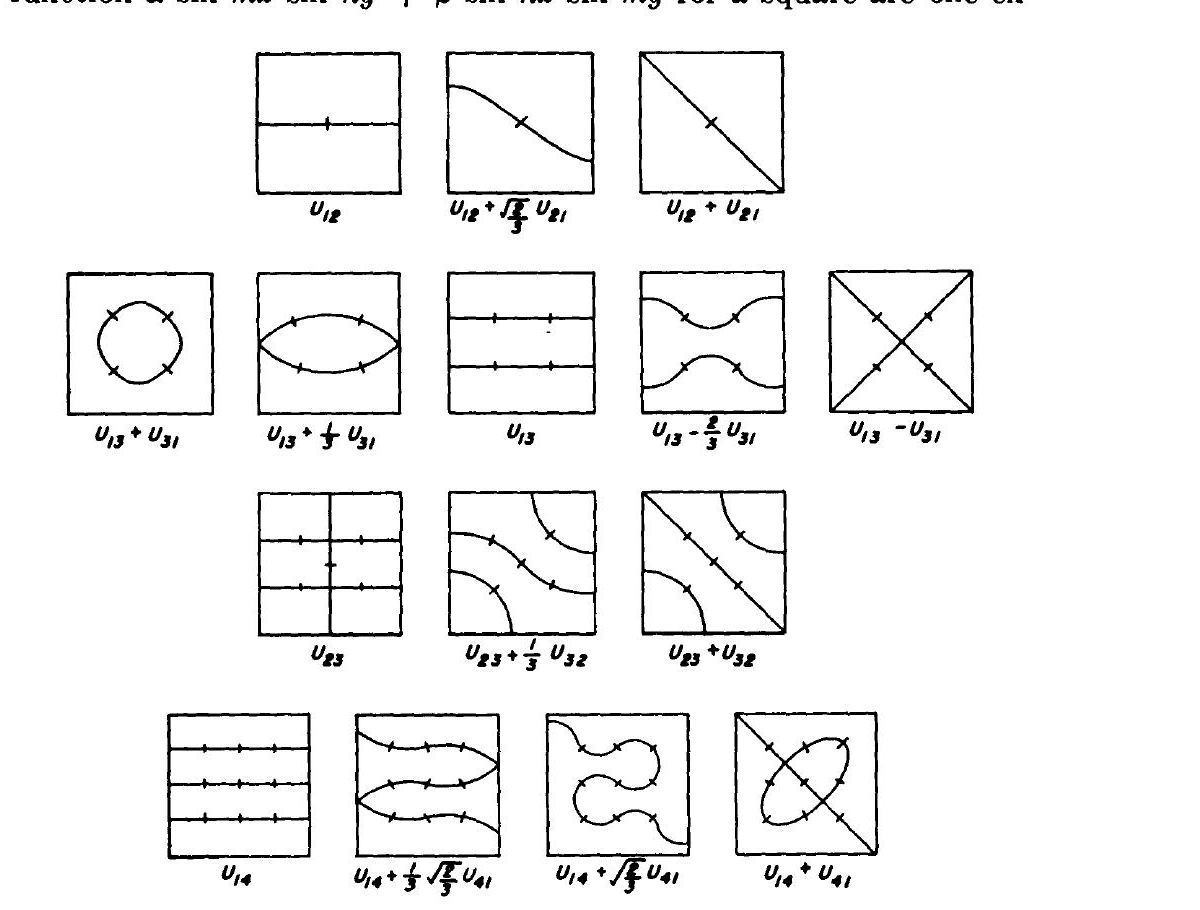
\includegraphics[width=.78\textwidth]{figures/ch05_fig3.png}\\[-.4em]
{\small Figure 3. Nodal lines for a square membrane.}
\end{center}

The above diagrams\footnote{A number are taken from the book by Pockels referred to in the bibliography.} illustrate a number of characteristic types. Here $u_{mn}$ denotes the function $\sin mx\sin ny$.

\subsection{Circular Membrane. Bessel Functions}
The circular membrane can also be treated explicitly; we assume its radius to be 1. The differential equation for its eigenvalue problem, in polar coordinates, takes the form
\begin{equation}\tag{26}
v_{rr}+\frac1r v_r+\frac1{r^2}v_{\theta\theta}+\lambda v=0,
\end{equation}
derived in Ch. IV, \S8, 2. If, as before, we consider the case of a stretched membrane, we have the boundary condition $v(1,\theta)=0$. If we attempt to solve equation (26) by setting $v(r,\theta)=f(r)h(\theta)$, we are led at once to the relation
\[
\frac{r^2\left(f''(r)+\frac1rf'(r)+\lambda f(r)\right)}{f(r)}
=-\frac{h''(\theta)}{h(\theta)}=\mathrm{const.}=c.
\]
Since $v(r,\theta)$ and hence $h(\theta)$ must be periodic functions of $\theta$ with period $2\pi$---otherwise $v$ would not be single-valued---it follows that $c$ has a value $c=n^2$, where $n$ is any non-negative integer. We thus obtain
\[
h(\theta)=a\cos n\theta+b\sin n\theta
\]
and, for $f(r)=y$, the differential equation
\begin{equation}\tag{27}
r^2y''+ry'+(r^2\lambda-n^2)y=0
\end{equation}
follows. The problem is to find eigenvalues $\lambda$ for which there exists a solution of this differential equation, continuous for $r=0$, which also satisfies the boundary condition $f(1)=0$. If we make the transformation $r\sqrt\lambda=\rho$ $(\lambda\ne0)$ or $kr=\rho$, setting $\lambda=k^2$, equation (27) takes the form
\begin{equation}\tag{28}
\frac{d^2y}{d\rho^2}+\frac1\rho\frac{dy}{d\rho}+\left(1-\frac{n^2}{\rho^2}\right)y=0.
\end{equation}
The solutions of this \emph{Bessel equation}, the so-called \emph{Bessel functions}, play a particularly important role in analysis and mathematical physics and will be the object of more detailed study in Chapter VII. At present, it should be pointed out that by writing $y$ as a power series $y(\rho)=\sum_{m=0}^\infty a_m\rho^m$ we obtain for (28) the solution
\[
\begin{aligned}
y(\rho)=J_n(\rho)
&=\frac{\rho^n}{2^n n!}\left\{1-\frac{\rho^2}{2(2n+2)}
+\frac{\rho^4}{2\cdot4(2n+2)(2n+4)}-\cdots\right\},
\end{aligned}
\]
which is called the \emph{Bessel function of $n$-th order}. The series converges for every value of $\rho$, as is shown by simple criteria; that is, the Bessel functions $J_n(\rho)$ are entire transcendental functions. In particular, for $n=0$ we have the series expansion
\[
J_0(\rho)=1-\frac{\rho^2}{2^2}+\frac{\rho^4}{2^2 4^2}-\frac{\rho^6}{2^2 4^2 6^2}+\cdots.
\]
We note the relation
\begin{equation}\tag{29}
J_0'(\rho)=-J_1(\rho)
\end{equation}
which follows immediately from the series expansion.

We can write the solutions of (27) in the form
\begin{equation}\tag{30}
y_n=J_n(kr)\qquad(k^2=\lambda),
\end{equation}
where the constant $k$ is to be determined by the boundary condition $y_n(1)=0$, that is, by the condition $J_n(k)=0$. Thus the eigenvalues $\lambda=k^2$ of (27) are the squares of the zeros of the Bessel functions. As regards the existence of these zeros, we shall show later that each function $J_n$ has, in fact, infinitely many real zeros, which we shall denote by $k_{n,m}$ $(m=1,2,3,\ldots)$. Using this notation we can write the eigenfunctions in the form
\[
J_n(k_{n,m}r)(\alpha\cos n\theta+\beta\sin n\theta).
\]
The constants $\alpha,\beta$ in this expression are still arbitrary, which indicates that, with the exception of the eigenfunctions belonging to $n=0$, all the eigenvalues are at least double since they have the associated linearly independent eigenfunctions $J_n\cos n\theta$ and $J_n\sin n\theta$. The \emph{nodal curves for these eigenfunctions are circles $\rho=\mathrm{const.}$ and radial lines $\theta=\mathrm{const.}$}, respectively. The eigenvibrations are represented by
\[
u=J_n(k_{n,m}r)(\alpha\cos n\theta+\beta\sin n\theta)
(a\cos k_{n,m}t+b\sin k_{n,m}t).
\]
If we assume the more general boundary condition $\partial u/\partial r=-\sigma u$, with constant $\sigma$, almost all of the above considerations remain unchanged. However, the boundary condition from which the eigenvalues are determined takes a somewhat different form, namely
\[
kJ_n'(k)=-\sigma J_n(k).
\]

The functions $J_n(k_{n,m}r)$ are the only eigenfunctions for the membrane. This can be proved by noting that every eigenfunction $v$ is a periodic function of $\theta$, with period $2\pi$, having continuous derivatives up to the second order. Hence $v$ can be expanded in a Fourier series
\[
v(r,\theta)=\sum_{n=-\infty}^{\infty}f_n(r)e^{in\theta}.
\]
Substituting this series in equation (26), we see at once that each individual term $f_n(r)e^{in\theta}$ satisfies the differential equation.

From the general expansion theorem it follows that a function $w(r,\theta)$ vanishing on the boundary and continuous together with its derivatives up to the second order in the interior of the circle, can be expanded in an absolutely and uniformly convergent series of the form
\[
w(r,\theta)=\sum_{n,m=0}^{\infty}a_{n,m}J_n(k_{n,m}r)\cos n(\theta-\theta_{n,m}).
\]
For example, if $w$ does not depend on $\theta$, this implies that an arbitrary function of $r$, which vanishes for $r=1$ and has continuous derivatives up to the second order in the interval $0\le r\le1$, can be expanded in this interval in terms of the Bessel functions $J_0(k_{0,m}r)$.

The \emph{orthogonality relation}
\[
\int_0^1rJ_n(k_{n,i}r)J_n(k_{n,j}r)\,dr=0\qquad(i\ne j)
\]
for the Bessel functions, or the functions (30), is obtained from the general orthogonality relation for the eigenfunctions of the equation of a membrane by integrating with respect to $\theta$. This relation may also be derived directly from equation (27) using the now familiar method. Furthermore, it is clear that orthogonality is preserved even under the more general boundary condition $kJ_n'(k)=-\sigma J_n(k)$.

To normalize the functions $J_n(k_{n,m}r)$ we shall use relation
\begin{equation}\tag{31}
2\int_0^1J_n^2(kr)r\,dr=J_n'^2(k),
\end{equation}
which is proved as follows: We multiply the differential equation for $J_n(kr)=y$, i.e. the equation
\[
(ry')'+\left(rk^2-\frac{n^2}{r}\right)y=0,
\]
by $ry'$, and integrate from $0$ to $r$. Integrating by parts this leads to the relation
\[
2k^2\int_0^r ry^2\,dr=(ry')^2+(r^2k^2-n^2)y^2,
\]
from which equation (31) follows for $r=1$, since $y(1)=J_n(k)=0$. Thus the functions
\[
\frac{\sqrt2}{J_n'(k_{n,m})}J_n(k_{n,m}r)
\]
are the \emph{normalized eigenfunctions} for equation (27). For further results in the theory of Bessel functions the reader is referred to Chapter VII and to monographs on the subject.

\subsection{Nonhomogeneous Membrane}
The generalized differential equation of the nonhomogeneous membrane,
\[
p\Delta u+p_xu_x+p_yu_y-qu=\rho(x,y)u_{tt},
\]
in which $p$ and $\rho$ are positive in $G$, leads to an eigenvalue problem analogous to the general Sturm-Liouville problem of \S3. This is the problem of determining the values of $\lambda$ for which the differential equation
\[
L[v]+\lambda\rho v=p\Delta v+p_xv_x+p_yv_y-qv+\lambda\rho v=0
\]
possesses a normalized solution satisfying prescribed homogeneous boundary conditions. With the aid of Green's formula
\[
\iint_G\bigl(v_2L[v_1]-v_1L[v_2]\bigr)\,dx\,dy
=\int_\Gamma p\left(v_2\frac{\partial v_1}{\partial n}-v_1\frac{\partial v_2}{\partial n}\right)ds=0
\]
[page 280, formula (5a)], we obtain the orthogonality relation
\[
\iint_G\rho v_iv_j\,dx\,dy=0
\]
for the eigenfunctions $v_i,v_j$ corresponding to distinct eigenvalues $\lambda_i,\lambda_j$. We should like to determine the eigenfunctions in such a way that the functions $\sqrt\rho\,v_i$ form an orthonormal system, i.e. so that
\[
\iint_G\rho v_i^2\,dx\,dy=1.
\]
In \S14 \emph{the existence of the eigenvalues and the completeness and expansion theorems} will be treated from a general point of view. These theorems assert that a function $f(x,y)$ which satisfies the boundary conditions and has continuous derivatives of first and second order can be expanded:
\[
f=\sum_{n=1}^{\infty}c_nv_n(x,y),
\qquad
c_n=\iint_G\rho f v_n\,dx\,dy.
\]

\section{The Vibrating Plate}
\subsection{General Remarks}
For the differential equation
\[
\Delta\Delta u+u_{tt}=0
\]
of the homogeneous vibrating plate, we obtain the eigenvalue equation
\begin{equation}\tag{32}
\Delta\Delta v-\lambda v=0,
\end{equation}
writing $u=v(x,y)g(t)$ with $g(t)=\alpha e^{\pm i\nu t}$ or $g(t)=a\cos\nu t+b\sin\nu t$, and $\lambda=\nu^2$. As boundary conditions we consider for example
\[
u=0,\qquad \frac{\partial u}{\partial n}=0;
\qquad\text{i.e.,}\qquad
v=0,\qquad \frac{\partial v}{\partial n}=0
\]
(\emph{clamped plate}). \emph{The orthogonality of two eigenfunctions corresponding to two distinct eigenvalues} is proved by the same method as before using Green's formula (\S1). The only essential difference is that now two homogeneous boundary conditions characterize the eigenvalue problem; this corresponds to the fact that the partial differential equation under consideration is of fourth order.

\subsection{Circular Boundary}
The problem for the plate is analytically more difficult than that for the membrane. It is not possible, for example, to treat the case of the rectangular boundary in terms of functions known explicitly. The only boundary which has been explicitly treated is the circle. Introducing polar coordinates $r,\theta$ we are once more led to Bessel functions. If we set $\lambda=k^4$, we can write the differential equation in symbolic form:
\[
(\Delta\Delta-k^4)v=0
\]
or
\[
(\Delta-k^2)(\Delta+k^2)v=0;
\]
the operator $\Delta$ is given by
\[
\Delta=\frac{\partial^2}{\partial r^2}+\frac1r\frac{\partial}{\partial r}+\frac1{r^2}\frac{\partial^2}{\partial\theta^2}.
\]
If we suppose that $v$ is expanded in a Fourier series,
\[
v=\sum_{n=-\infty}^{\infty}y_n(r)e^{in\theta},
\]
then each term of the series must satisfy the differential equation; in other words, $y_n$ must be a solution of
\[
\left(\frac{d^2}{dr^2}+\frac1r\frac d{dr}-\frac{n^2}{r^2}-k^2\right)
\left(\frac{d^2}{dr^2}+\frac1r\frac d{dr}-\frac{n^2}{r^2}+k^2\right)y=0.
\]
We can find two linearly independent solutions of this differential equation which are regular for $r=0$: $J_n(kr)$ and $J_n(ikr)$, where $i=\sqrt{-1}$. Thus the function
\[
\begin{aligned}
v(r,\theta)={}&J_n(kr)(a_1\cos n\theta+b_1\sin n\theta)\\
&+J_n(ikr)(a_2\cos n\theta+b_2\sin n\theta)
\end{aligned}
\]
is a solution of (32). To satisfy the boundary conditions $v(1,\theta)=0$, $v_r(1,\theta)=0$, we must have
\[
J_n(k)a_1+J_n(ik)a_2=0,
\qquad
J_n(k)b_1+J_n(ik)b_2=0,
\]
\[
J_n'(k)a_1+iJ_n'(ik)a_2=0,
\qquad
J_n'(k)b_1+iJ_n'(ik)b_2=0.
\]
Hence, the eigenfrequency $k$ satisfies the transcendental equation
\[
\frac{J_n'(k)}{J_n(k)}=\frac{iJ_n'(ik)}{J_n(ik)}
\]
in which the imaginary unit $i$ no longer really occurs, as is shown by the series expansions of the Bessel functions. For details the reader is again referred to the literature.

\section{General Remarks on the Eigenfunction Method}
Let us now examine the essential features of the method illustrated by the foregoing examples.

\subsection{Vibration and Equilibrium Problems}
Let $G$ be a domain of the independent space variables $x,\ldots$, i.e. an interval on the $x$-axis or a domain either in the $x,y$-plane or in $x,y,z$-space which has a piecewise smooth boundary $\Gamma$. Suppose the state of a continuum filling $G$ is characterized by a function $u(x,\ldots;t)$ which vanishes identically if the system is in stable equilibrium. Let $L[u]$ be a self-adjoint linear differential expression in the independent variables $x,\ldots$, defined in $G$, which arises from the variation of the system's potential energy. Let $\rho(x,\ldots)$ represent the mass density at any point of $G$ and let $Q(x,\ldots;t)$ represent a given external force. We wish to find a solution of the differential equation
\begin{equation}\tag{33}
L[u]=\rho u_{tt}-Q
\end{equation}
which satisfies prescribed homogeneous time-independent boundary conditions on the boundary $\Gamma$ of $G$, and which corresponds to a prescribed initial state defined by
\[
u(x,\ldots;0)=\varphi(x,\ldots),
\qquad
u_t(x,\ldots;0)=\psi(x,\ldots).
\]
All occurring derivatives are assumed to be continuous in $G$.

The case of equilibrium corresponds to the special assumption that all functions considered are independent of $t$ (and no initial conditions are given). Instead of a mixed initial-boundary value problem for vibration, we then obtain a boundary value problem for equilibrium.

Among the free motions characterized as the solutions of the homogeneous differential equation
\begin{equation}\tag{33a}
L[u]=\rho u_{tt}
\end{equation}
which satisfy the prescribed homogeneous boundary conditions, we distinguish the eigenvibrations by requiring \emph{synchronism}: $u=v(x,\ldots)g(t)$. Each such eigenvibration is associated with a constant value $\lambda$, an eigenvalue, with the property $\ddot g+\lambda g=0$; hence
\[
g(t)=a\cos\sqrt\lambda\,t+b\sin\sqrt\lambda\,t,
\]
and
\begin{equation}\tag{34}
L[v]+\lambda\rho v=0,
\end{equation}
where $v$ must satisfy the boundary conditions for $u$ given above. The \emph{eigenvalue problem} is to determine values of the parameter $\lambda$ (eigenvalues) for which the homogeneous differential equation (34) has nontrivial solutions (eigenfunctions) under the prescribed boundary conditions. The vibration satisfying the original equation (33a) is then represented by
\[
u=(a\cos\sqrt\lambda\,t+b\sin\sqrt\lambda\,t)v(x,\ldots).
\]

In the case of a finite domain $G$ the following statements are in general true: The eigenvalues $\lambda$ form a denumerably infinite sequence $\lambda_1,\lambda_2,\ldots$. There exists a \emph{system of associated eigenfunctions} $v_1,v_2,\ldots$ which is \emph{complete} in the sense of Ch. II, \S1 and which satisfies the orthogonality relations\footnote{The notation $\int_G f\,d\tau$ means the integral of the function $f(x,\ldots)$ over the domain $G$.}
\[
\int_G\rho v_iv_k\,d\tau=0\qquad(i\ne k),
\]
\[
\int_G\rho v_i^2\,d\tau=1.
\]
Moreover, the \emph{expansion theorem} holds: Every function $w$ with continuous $L[w]$ which satisfies the prescribed homogeneous boundary conditions may be expanded in an absolutely and uniformly convergent series in the eigenfunctions:
\[
w=\sum_{i=1}^{\infty}c_iv_i,
\qquad
c_i=\int_G\rho wv_i\,d\tau.
\]
On the basis of these properties---which must be proved for each problem (cf. \S14)---we obtain an infinite sequence of eigenvibrations
\[
(a_i\cos\sqrt{\lambda_i}\,t+b_i\sin\sqrt{\lambda_i}\,t)v_i(x,\ldots).
\]
From these eigenvibrations we obtain the solutions of the initial value problem for (33a) by superposition if we choose the constants $a_i$ and $b_i$ suitably:
\[
a_i=\int_G\rho\varphi v_i\,d\tau,
\qquad
b_i=\frac1{\sqrt{\lambda_i}}\int_G\rho\psi v_i\,d\tau.
\]
For the nonhomogeneous equation (33) with homogeneous boundary conditions---as we saw in \S\S1, 2, there is no loss of generality in assuming homogeneous boundary conditions for a nonhomogeneous equation---the solution $u(x,\ldots;t)$ is found by determining its expansion coefficients $\gamma_i(t)$ with respect to the $v_i$. To this end we multiply equation (33) by $v_i$, integrate over $G$, and transform the left side by Green's formula (5a), \S1, taking the boundary conditions into consideration; using (34) we obtain
\[
\ddot\gamma_i+\lambda_i\gamma_i=Q_i(t),
\]
where $Q_i(t)$ is the given expansion coefficient of $Q(x,\ldots;t)\rho^{-1}$ with respect to the $v_i$. A special solution of this equation for $\gamma_i$ is given by
\[
\gamma_i=\frac1{\sqrt{\lambda_i}}\int_0^tQ_i(\tau)\sin\sqrt{\lambda_i}(t-\tau)\,d\tau.
\]
The function formed using these expansion coefficients is a particular solution of (33), and all other solutions are obtained by adding a solution of (33a). Thus the initial value problem under consideration is reduced to the problem of solving the homogeneous equation (33a).

In terms of eigenfunctions we can also solve the equilibrium problem, i.e. the boundary value problem for the differential equation
\[
L[u]=-Q(x,\ldots)
\]
with homogeneous boundary conditions. In the same way we obtain the equation $\lambda_i\gamma_i=Q_i$ for the expansion coefficients of the desired solution $u$ with respect to the $v_i$, i.e.
\[
\gamma_i=\frac1{\lambda_i}\int_GQv_i\,d\tau.
\]
Hence, by the expansion theorem, the solution is given by
\[
u=\sum_{i=1}^{\infty}\frac{v_i}{\lambda_i}\int_GQv_i\,d\tau.
\]
If we could interchange summation and integration in this expression we would arrive at a function
\[
K(x,\ldots;\xi,\ldots)=\sum_{i=1}^{\infty}\frac{v_i(x,\ldots)v_i(\xi,\ldots)}{\lambda_i}
\]
such that the solution of the boundary value problem could be written in the form
\[
u(x,\ldots)=\int_GQ(\xi,\ldots)K(x,\ldots;\xi,\ldots)\,d\tau,
\]
where the integration is to be carried out with respect to the variables $\xi,\ldots$. This function $K$, ``\emph{Green's function}'' of $L[u]$, will be characterized in \S14 in a quite different manner and will form the basis for a more detailed investigation reaching beyond the formal structure of the present method.

\subsection{Heat Conduction and Eigenvalue Problems}
The theory of heat conduction also leads to eigenvalue problems. If the units of time and length are suitably chosen, the differential equation of heat conduction takes the form
\[
L[u]=u_t,
\]
where $u$ denotes the temperature as a function of position $(x,y,z)$ and time $t$. The radiation of heat from a homogeneous body $G$ with surface $\Gamma$ into an infinite medium of constant temperature zero is characterized at the surface $\Gamma$ by a boundary condition of the form
\[
\frac{\partial u}{\partial n}+\sigma u=0
\]
where $\sigma$ is a positive physical constant. This condition states that the rate of change of temperature in the direction of the inner normal is proportional to the jump in temperature from the exterior to the interior of the body. We seek a solution of the equation of heat conduction which satisfies this boundary condition and prescribed initial conditions at the time $t=0$.

We write $u$ in the form $u=v(x,y,z)g(t)$ and obtain at once the equation
\[
\frac{L[v]}{v}=\frac{\dot g}{g}=-\lambda.
\]
We thus have the following eigenvalue problem for $v$: $L[v]+\lambda v=0$ in $G$ and $\partial v/\partial n+\sigma v=0$ on the surface $\Gamma$; for a given eigenvalue $\lambda$ and its eigenfunction $v$ the corresponding solution of the differential equation has the form
\[
u=av e^{-\lambda t}.
\]
By the eigenfunction expansion theorem we can again make the solution satisfy a given initial state; then $u(x,y,z;0)$ equals an arbitrarily prescribed function $\varphi(x,y,z)$, which is continuous in $G$ together with its derivatives of first and second order and satisfies the boundary condition. For, if the normalized eigenfunctions $v_1,v_2,\ldots$ and their associated eigenvalues $\lambda_1,\lambda_2,\ldots$ form a complete system, the desired solution is given by the formula
\[
u(x,y,z;t)=\sum_{n=1}^{\infty}c_nv_n(x,y,z)e^{-\lambda_nt}
\]
where
\[
c_n=\iiint_G\varphi v_n\,dx\,dy\,dz.
\]
Incidentally, the positive character of the eigenvalues $\lambda$ implies that the solution $u(x,y,z;t)$ approaches zero asymptotically as $t$ increases as must be expected from the physical meaning of the problem.

If, in place of the homogeneous equation of heat conduction, we consider the inhomogeneous equation
\[
L[u]=u_t-Q(x,y,z)
\]
(in which we assume that the given function $Q$ does not depend on the time) and impose the same boundary conditions on $u$ as above, we obtain by our general method a solution $u(x,y,z;t)$ which, as $t\to\infty$, goes over into the solution of the corresponding boundary value problem for the equation
\[
L[u]=-Q(x,y,z).
\]

\section{Vibrations of Three-dimensional Continua. Separation of Variables}
In the theory of vibrations of three-dimensional continua, e.g. in acoustics, elasticity, or electrodynamics, homogeneous boundary value problems arise for the equation
\[
\Delta u=u_{tt}
\]
where $\Delta u$ is the potential expression in three variables; we are led to eigenvalue problems of the form
\[
\Delta u+\lambda u=0
\]
with corresponding homogeneous boundary conditions.

It often happens that the particular shape of the fundamental domain permits a further separation of variables for the solutions of this eigenvalue problem and thus leads to new eigenvalue problems involving fewer independent variables.

An example is given by a cylindrical domain erected over the domain $G$ of the $x,y$-plane and bounded by the planes $z=0$ and $z=\pi$. Let us take $u=0$ as a boundary condition. By means of the substitution $u=f(z)v(x,y)$ this problem can be reduced immediately to the corresponding problem for the plane domain $G$, and we obtain
\[
-\frac{f''}{f}=\frac{\Delta v}{v}+\lambda=k=\mathrm{const.},
\qquad
f=\sin\sqrt{k}\,z
\]
where $k=1^2,2^2,3^2,\ldots$. The equation for $v$ is $\Delta v+(\lambda-n^2)v=0$; here the eigenvalues differ from those for the plane domain $G$ only by the terms $+n^2$\ctnote{由前式 $\Delta v+(\lambda-n^2)v=0$，若平面域对应的特征值记为 $\mu$，则 $\lambda=\mu+n^2$。原文此处印作 ``$-n^2$''，与下一句长方体的特征值 $l^2+m^2+n^2$ 也不相容。}, and the eigenfunctions are identical with those for the plane domain $G$.

From the completeness of the system of eigenfunctions, it follows, as in previous cases, that we thus obtain all the eigenfunctions of the cylinder under the given boundary conditions.

If the cylinder is erected over a rectangular domain, we have a rectangular parallelepiped; e.g., for the cube $0\le x,y,z\le\pi$, we obtain the eigenvalues $l^2+m^2+n^2$ $(l,m,n=1,2,3,\ldots)$ and the eigenfunctions $\sin lx\sin my\sin nz$.

As a further example, we consider the \emph{vibration equation for the spherical domain $x^2+y^2+z^2\le1$} of radius 1. If we introduce polar coordinates $r,\theta,\varphi$, the vibration equation takes the form (cf. Ch. IV, \S8, 2)
\[
\begin{aligned}
\Delta u+\lambda u
={}&\frac1{r^2\sin\theta}\left[
\frac{\partial}{\partial r}(r^2u_r\sin\theta)
+\frac{\partial}{\partial\varphi}\left(\frac{u_\varphi}{\sin\theta}\right)
+\frac{\partial}{\partial\theta}(u_\theta\sin\theta)
\right]+\lambda u=0.
\end{aligned}
\]
If we look for a solution of the form $u=Y(\theta,\varphi)f(r)$, we obtain
\[
\frac{(r^2f')'+\lambda r^2f}{f}
=-\frac1{Y\sin\theta}\left[
\frac{\partial}{\partial\varphi}\left(\frac{Y_\varphi}{\sin\theta}\right)
+\frac{\partial}{\partial\theta}(Y_\theta\sin\theta)
\right]=k,
\]
where $k$ is a constant. The value of $k$ must be determined in such a way that the differential equation
\[
\Delta^*Y+kY
=\frac1{\sin\theta}\left[
\frac{\partial}{\partial\varphi}\left(\frac{Y_\varphi}{\sin\theta}\right)
+\frac{\partial}{\partial\theta}(Y_\theta\sin\theta)
\right]+kY=0
\]
has a solution which is continuous on the entire surface of the sphere. Therefore, this solution must be periodic in $\varphi$, of period $2\pi$, and regular at $\theta=0$ and $\theta=\pi$ (i.e., at both these points it must approach a limit independent of $\varphi$). We shall see in Ch. VII, \S5 that this requirement is satisfied only for the values $k=n(n+1)$ $(n=0,1,2,\ldots)$; in this case the solutions are the \emph{spherical harmonics} $Y_n(\theta,\varphi)$ (see also \S9). We have for $f(r)$ the equation
\[
(r^2f')'-n(n+1)f+\lambda r^2f=0;
\]
the solutions of this equation which are regular at $r=0$ are the functions
\[
S_n(\sqrt\lambda r)=\frac{J_{n+\frac12}(\sqrt\lambda r)}{\sqrt r}
\]

(cf. \S5 and \S10). We now have to determine the parameter $\lambda$ from the boundary condition. For example, if the boundary condition is given by $u=0$, then $\lambda$ is determined by the equation
\[
J_{n+\frac12}(\sqrt\lambda)=0;
\]
denoting the roots of this equation by $\lambda_{n,1},\ldots$, we obtain solutions of the form
\[
u=Y_n(\theta,\varphi)S_n(\sqrt{\lambda_{n,k}}\,r)
\]
for the boundary value problem. In Ch. VII, \S5 we shall prove that these solutions constitute a complete orthogonal system, and hence represent all the eigenfunctions and eigenvalues for our differential equation problem.

\section{Eigenfunctions and the Boundary Value Problem of Potential Theory}
The boundary value problem of potential theory is the problem of determining a function $u$ which satisfies the differential equation $\Delta u=0$ in the interior of a domain $G$, and assumes prescribed values on the boundary. In \S\S1, 2, it was pointed out that we may instead solve the nonhomogeneous equation $\Delta u=f$ with the associated boundary condition $u=0$. We could investigate the latter problem by the method of \S7, expanding $f$ and $u$ in terms of the eigenfunctions for the equation
\[
\Delta v+\lambda v=0.
\]
However, for suitable special domains $G$ we can proceed more simply: by separating the variables one can reduce the number of independent variables in the problem. This procedure will be illustrated by a number of important examples.

\subsection{Circle, Sphere, Spherical Shell}
Consider first the case of two independent variables $x,y$; let $G$ be the circle of radius 1 about the origin. If we transform the expression $\Delta u$ to polar coordinates $r,\varphi$, we have the following boundary value problem: to solve the equation
\[
r(ru_r)_r+u_{\varphi\varphi}=0
\]
with preassigned boundary values $u(1,\varphi)=f(\varphi)$; here $f(\varphi)$ is a continuous periodic function of period $2\pi$ with a piecewise continuous first derivative. If we attempt to find solutions of the homogeneous equation---for the moment ignoring the boundary condition---which can be written in the form $u=v(r)w(\varphi)$, we are led in the usual manner to an eigenvalue problem
\[
w''+\lambda w=0;
\]
the boundary conditions are the periodicity conditions $w(0)=w(2\pi)$, $w'(0)=w'(2\pi)$. The eigenvalues for this problem are given by $\lambda=n^2$ (integral $n$), the associated eigenfunctions are given by
\[
w=a_n\cos n\varphi+b_n\sin n\varphi.
\]
For $v(r)$ we obtain the differential equation
\[
r(rv')'-n^2v=0,
\]
of which $v=r^n$ and $v=r^{-n}$ are linearly independent solutions. Thus we obtain particular solutions of the original equation, which are regular in the unit circle and have the form
\[
(a_n\cos n\varphi+b_n\sin n\varphi)r^n,
\]
where the constants $a_n$ and $b_n$ are arbitrary. (These solutions can also be characterized as solutions of the differential equation $\Delta u=0$ which are integral rational functions of $x$ and $y$ and homogeneous of the $n$-th degree.)

According to the theory of Fourier series we can obtain the desired solution of the boundary value problem by the process of superposition,
\[
u=\sum_{n=0}^{\infty}r^n(a_n\cos n\varphi+b_n\sin n\varphi),
\]
with the coefficients $a,b$ taken from the series expansion of the preassigned boundary values (cf. Ch. IV, \S2, p. 179).

The situation is quite similar in three dimensions, where we consider the unit sphere $x^2+y^2+z^2\le1$ for $G$; then \emph{Laplace's spherical harmonics} occur instead of the trigonometric functions. In fact, if we transform the differential equation to polar coordinates $r,\theta,\varphi$ (cf. pages 225 and 314) we obtain the equation
\[
(r^2u_r)_r+\frac1{\sin^2\theta}u_{\varphi\varphi}
 +\frac1{\sin\theta}(u_\theta\sin\theta)_\theta=0,
\]
which for $u=v(r)Y(\theta,\varphi)$ leads to the equation
\begin{equation}
(r^2v')'-\lambda v=0.
\tag{35}
\end{equation}
The general solution of (35) has the form
\[
v=c_1r^{\alpha_1}+c_2r^{\alpha_2}
\]
where $c_1$ and $c_2$ are arbitrary constants and $\alpha_1,\alpha_2$ denote roots of the quadratic equation
\[
\alpha(\alpha+1)=\lambda.
\]
For $Y$ we obtain the same eigenvalue problem as in \S8, given by the differential equation
\begin{equation}
\Delta^*Y+\lambda Y
=\frac1{\sin\theta}\left[\frac1{\sin\theta}Y_{\varphi\varphi}+(Y_\theta\sin\theta)_\theta\right]+\lambda Y=0.
\tag{36}
\end{equation}
where $\lambda$ must be determined in such a way that the equation has a nontrivial solution with continuous derivatives up to the second order over the entire sphere.

To justify our requirement that $Y(\theta,\varphi)$ be regular even at the poles $\theta=0$, $\theta=\pi$ of the sphere we observe that the operator $\Delta$ is invariant under rotations of the coordinate system; for $r=1$, $\Delta$ becomes $\Delta^*$, hence $\Delta^*$ is also invariant under coordinate rotations. The singularities of equation (36) at the points $\theta=0$, $\theta=\pi$ are a consequence of the particular choice of the coordinate system. It is therefore natural to require that the poles of the sphere be regular points of the function $Y$. (In other words, $Y$ as a function of position on the sphere should satisfy the same regularity conditions everywhere.)

The eigenvalues $\lambda$ and associated eigenfunctions $Y$ are most easily determined by investigating those solutions $u=U_n$ of $\Delta u=0$ which are integral and rational in $x,y,z$ and homogeneous of degree $n$; this investigation is analogous to \S8. If we write these solutions in polar coordinates in the form $U_n=r^nY_n(\theta,\varphi)$, we see that the $Y_n$ are solutions of equation (36). The eigenvalues corresponding to the $2n+1$ functions $Y_n(\theta,\varphi)$ are found to be
\[
\lambda=n(n+1).
\]
It will be shown in Ch. VII, \S5 that the functions $Y_n$ defined in this manner constitute the totality of eigenfunctions of our problem.

Furthermore, it will be possible to give a proof for the completeness and expansion theorems which is similar to that used for the Sturm--Liouville functions. From the expansion theorem it follows that by superposition of solutions:
\[
u=\sum_{n=0}^{\infty}a_nr^nY_n,
\]
we can find a solution of $\Delta u=0$ which assumes prescribed values on the surface of the sphere.

Not only the function $u=r^nY_n$ but also $u=r^{-(n+1)}Y_n$, which has a singularity at zero, is a solution of $\Delta u=0$. Thus, by superposition of solutions of the form $r^nY_n$ and $r^{-(n+1)}Y_n$, one can find a solution of $\Delta u=0$ which assumes prescribed values on two concentric spheres and is regular in the intermediate shell.

If in particular we consider those spherical harmonics which depend only on $\theta$ and not on $\varphi$ (i.e., if we assume $Y_\varphi=0$) the differential equation takes the form
\[
\frac1{\sin\theta}(Y_\theta\sin\theta)_\theta+\lambda Y=0;
\]
performing the transformation $x=\cos\theta$, this equation becomes the equation for the Legendre polynomials (cf. eq. (20), Ch. II). The Legendre polynomials $P_n(\cos\theta)$ are a special case of spherical harmonics.

We obtain a generalization of the spherical harmonics if we consider an arbitrary domain $G$ on the surface of the sphere and attempt to solve the differential equation (36)
\[
\Delta^*Y+\lambda Y=0
\]
for a function $Y(\theta,\varphi)$, regular in $G$, which satisfies homogeneous boundary conditions on the boundary of $G$; for example, the function may be required to vanish there. Eigenfunctions $Y_1,Y_2,\ldots$ belonging to this domain are called spherical surface harmonics. It follows from the above calculations that, if $\alpha$ and $\lambda$ satisfy the relation
\[
\alpha(\alpha+1)=\lambda,
\]
the function $r^\alpha Y(\theta,\varphi)=u(x,y,z)$ is a solution of the differential equation $\Delta u=0$ which is continuous, except possibly at the origin, in the cone with $G$ as base and the center of the sphere as vertex.

The equation $\Delta^*Y+\lambda Y=0$ for spherical surface harmonics is a special case of the general differential equation
\[
\begin{aligned}
\Delta^*Y+\lambda Y
={}&\frac1{\sqrt{eg-f^2}}
\left(
\frac{\partial}{\partial y}
\frac{e\,\partial Y/\partial y-f\,\partial Y/\partial x}{\sqrt{eg-f^2}}
+\frac{\partial}{\partial x}
\frac{g\,\partial Y/\partial x-f\,\partial Y/\partial y}{\sqrt{eg-f^2}}
\right)
+\lambda Y=0
\end{aligned}
\]
corresponding to an arbitrary curved surface with the line element $ds^2=e\,dx^2+2f\,dx\,dy+g\,dy^2$. In Ch. IV, \S8, 2 we noted that this equation is invariant. It can be considered as the equation of vibration of a ``curved membrane'' lying on the surface. In the case of a sphere it becomes equation (36) if polar coordinates are introduced.\footnote{Cf. W. Thomson and P. G. Tait, \emph{Treatise on Natural Philosophy}, Vol. I, pp. 171--218, Cambridge University Press, Cambridge, 1886.}

\subsection{Cylindrical Domain}
A further example of a region for which the boundary value problem of potential theory may be solved explicitly is given by a cylinder erected over the domain $G$ of the $x,y$-plane which is bounded by the planes $z=0$ and $z=\pi$. We assume that the boundary values are identically zero on the vertical surface of the cylinder and that they are given on the plane bases by arbitrary twice continuously differentiable functions which vanish on the boundaries $\Gamma$. We now seek solutions of $\Delta u=0$ of the form $u=f(z)v(x,y)$ and obtain as above the conditions $f''/f=-\Delta v/v=\lambda$, i.e., differential equations for $f$ and for $v$ in which $\lambda$ is to be determined in such a way that an eigenfunction $v(x,y)$ which vanishes on $\Gamma$ exists. If $v_1,v_2,\ldots$ are all the eigenfunctions, with corresponding eigenvalues $\lambda_1,\lambda_2,\ldots$, then, by the expansion theorem, we can determine the constants $a_n,b_n$ in such a way that the infinite series
\[
\sum_{n=1}^{\infty}\left(a_ne^{\sqrt{\lambda_n}z}+b_ne^{-\sqrt{\lambda_n}z}\right)v_n(x,y)
\]
takes on the given boundary values for $z=0$ and for $z=\pi$. Hence this series is the solution of our boundary value problem, provided that it converges uniformly together with the series obtained from it by repeated termwise differentiation with respect to any of the variables $x,y,z$.

\subsection{The Lam\'e Problem}
Essentially, the most general case in which separation of variables helps to reduce the boundary value problem of potential theory to an eigenvalue problem for functions of a single variable is the case of a \emph{confocal rectangular parallelepiped}. By the latter we mean a domain bounded by a portion of each of two ellipsoids, a portion of each of two hyperboloids of one sheet and a portion of each of two hyperboloids of two sheets, all belonging to the same confocal family
\[
\frac{x^2}{s-e_1}+\frac{y^2}{s-e_2}+\frac{z^2}{s-e_3}=1
\]
(cf. Ch. IV, \S8, 3). \emph{Almost all the boundary value problems which are usually treated explicitly may be considered as special or limiting cases of this ``Lam\'e'' problem.} If we introduce elliptic coordinates $\rho=f(u)$, $\sigma=g(v)$, $\tau=h(w)$ in accordance with the notation of Chapter IV, the potential equation $\Delta T=0$ becomes
\[
\Delta T=
\frac{[g(v)-h(w)]T_{uu}+[f(u)-h(w)]T_{vv}+[f(u)-g(v)]T_{ww}}
{[g(v)-h(w)][f(u)-h(w)][f(u)-g(v)]}=0.
\]
Evidently, solutions of the form
\[
T=U(u)V(v)W(w)
\]
can be obtained if we can find two constants $\lambda,\mu$ which satisfy the following three ordinary differential equations
\begin{align}
U''+[\lambda f(u)+\mu]U&=0, \tag{37}\\
V''-[\lambda g(v)+\mu]V&=0, \tag{38}\\
W''+[\lambda h(w)+\mu]W&=0, \tag{39}
\end{align}
where the variables $u,v,w$ lie in the intervals
\[
u_2\le u\le u_1,\qquad v_2\le v\le v_1,\qquad w_2\le w\le w_1
\]
determined by the conditions
\[
\rho_2\le f(u)\le\rho_1,\qquad
\sigma_2\le g(v)\le\sigma_1,\qquad
\tau_2\le h(w)\le\tau_1.
\]
Thus the parallelepiped is given by conditions of the form
\[
\rho_1\ge\rho\ge\rho_2\ge\sigma_1\ge\sigma\ge\sigma_2\ge\tau_1\ge\tau\ge\tau_2.
\]
Using the coordinates $\rho,\sigma,\tau$ instead of $u,v,w$ and denoting the independent variable by $s$ and the dependent variable by $Y$, we can write equations (37), (38), and (39) in the form
\[
\varphi(s)\frac{d^2Y}{ds^2}+\frac{\varphi'(s)}2\frac{dY}{ds}+(\lambda s+\mu)Y=0,
\]
where we have set
\[
4(s-e_1)(s-e_2)(s-e_3)=\varphi(s).
\]
The solutions of this equation (the \emph{Lam\'e equation}) are functions which depend on the choice of the constants $\lambda,\mu$, and in general cannot be expressed in terms of the elementary transcendental functions. They are called \emph{Lam\'e functions} and have been extensively investigated, even though relatively few means for their numerical calculation have been developed. Here we state only the associated eigenvalue problem. Clearly the boundary value problem of potential theory can be solved for a confocal parallelepiped if it can be solved for the special case in which the given boundary values vanish on five of the six faces. Then the solution of the general boundary value problem is the sum of six such special solutions. Suppose, for example, that for $\tau=\tau_2$ nonzero boundary values have been assigned. We seek the solutions $U,V,W$ of the Lam\'e equations (37), (38), (39) for which the relations $U(u_1)=U(u_2)=V(v_1)=V(v_2)=W(w_1)=0$ hold but place no condition on $W(w_2)$. The product
\[
T=U(u)V(v)W(w)
\]
will then be a solution of $\Delta T=0$ which vanishes for $\rho=\rho_2$, $\rho=\rho_1$, $\sigma=\sigma_2$, $\sigma=\sigma_1$, $\tau=\tau_1$. However, as we shall see, the given conditions cannot be satisfied for an arbitrary choice of $\lambda,\mu$. Thus, we have a new eigenvalue problem, a so-called \emph{two-parameter eigenvalue problem}, in which we must determine pairs of associated eigenvalues $\lambda_i,\mu_i$ for which equations (37) and (38) have solutions that vanish for $u=u_1,u=u_2$ and $v=v_1,v=v_2$, respectively.

The situation in this eigenvalue problem is similar to that in the ordinary one-parameter problem: \emph{There exist infinitely many pairs of eigenvalues $\lambda_i,\mu_i$ and corresponding solutions $U_i,V_i$ of the eigenvalue problem. Every function of $u,v$ which is continuous in the rectangle $u_2\le u\le u_1$, $v_2\le v\le v_1$ together with its derivatives up to the second order, and which vanishes on the boundary of the rectangle, can be expanded in an absolutely and uniformly convergent series of the form}
\[
\sum_{i=1}^{\infty}c_iU_i(u)V_i(v)
\]
\emph{where the summation is over all Lam\'e products $U_i(u)V_i(v)$ which correspond to the eigenvalue pairs. Furthermore, Lam\'e products which correspond to different eigenvalue pairs satisfy the orthogonality relation}
\[
\int_{u_2}^{u_1}\int_{v_2}^{v_1}[f(u)-g(v)]U_i(u)V_i(v)U_k(u)V_k(v)\,dv\,du=0.
\]

To solve the boundary value problem, the next step is to associate to each pair of eigenfunctions $U_i,V_i$ a function $W_i(w)$ which satisfies equation (39) for $\lambda=\lambda_i$ and $\mu=\mu_i$ and vanishes for $w=w_1$. (The existence of one such solution follows from general existence theorems in the theory of differential equations.) The $W_i(w)$ do not vanish for $w=w_2$, for otherwise $T=UVW$ would be a nonvanishing solution of $\Delta T=0$ with vanishing boundary values, which contradicts elementary facts of potential theory.

The boundary values assigned on $w=w_2$ can then be expanded in a series of the form
\[
\sum_{i=1}^{\infty}a_iW_i(w_2)U_i(u)V_i(v),
\]
and the series
\[
\sum_{i=1}^{\infty}a_iU_i(u)V_i(v)W_i(w)
\]
represents the desired solution of the boundary value problem of potential theory for our parallelepiped. The above formulation of the expansion theorem apparently implies that the prescribed boundary values of $T$ should vanish on all the edges of the parallelepiped. Further investigation would show, however, that this restriction need not actually be imposed.

Our two-parameter eigenvalue problem is easily reduced to a one-parameter problem for a partial differential equation. Let us set $Z(u,v)=U(u)V(v)$, where $U(u)$ is a solution of equation (37) and $V(v)$ a solution of equation (38). If we multiply the first of these equations by $V$, the second by $U$, and add, we obtain the partial differential equation
\begin{equation}
Z_{uu}+Z_{vv}+\lambda[f(u)-g(v)]Z=0
\tag{40}
\end{equation}
for the function $Z(u,v)$. This differential equation might have been obtained directly from $\Delta T=0$ by writing $T=Z(u,v)W(w)$. Evidently, the eigenvalue $\lambda=\lambda_i$ and the associated eigenfunction $Z_i=U_i(u)V_i(v)$ solve the eigenvalue problem of this differential equation for the rectangle $G$: $u_2\le u\le u_1$, $v_2\le v\le v_1$ under the boundary condition $Z=0$. Since equation (40) has the form $\Delta Z+\lambda\rho Z=0$, where the function $\rho=f(u)-g(v)$ is positive throughout the rectangle $G$, this eigenvalue problem is of the type considered above, and we have analogous questions of existence of eigenfunctions and validity of an eigenfunction expansion theorem. These questions will be discussed later.\footnote{See \S\S14, 15.} At present we postulate that, for the rectangle $G$, infinitely many eigenvalues $\lambda_1,\lambda_2,\ldots$ exist together with associated eigenfunctions $Z_1,Z_2,\ldots$ which vanish at the boundary; arbitrary functions can be expanded in terms of the $\lambda_i$ and $Z_i$ as described above. Now we shall show that all the eigenfunctions $Z_i$ are Lam\'e products $U(u)V(v)$, or the sum of at most a finite number of Lam\'e products belonging to the same eigenvalue $\lambda$.

Proof: let $\lambda_1,\lambda_2,\ldots$ and $Z_1,Z_2,\ldots$ denote the complete system of eigenvalues and corresponding eigenfunctions for (40). Corresponding to any eigenvalue $\lambda_h$, we consider the ordinary differential equation
\[
\frac{d^2X}{du^2}+[\lambda_hf(u)+\mu]X=0
\]
with the boundary condition $X=0$ for $u=u_1$ and $u=u_2$. We denote the infinitely many associated eigenvalues and the normalized eigenfunctions by $\mu_1,\mu_2,\ldots$ and $X_1,X_2,\ldots$, respectively. Given any function which vanishes for $u=u_1$ and $u=u_2$ and is continuous with its derivatives up to the second order in the interval $u_2\le u\le u_1$, we can expand it in terms of these eigenfunctions. This is true in particular for the function $Z(u,v)$ which depends on an additional parameter $v$. We write the expansion in the form
\[
Z(u,v)=\sum_{n=1}^{\infty}Y_n(v)X_n(u),
\]
where
\[
Y_n(v)=\int_{u_2}^{u_1}Z(u,v)X_n(u)\,du
\]
and differentiate $Y_n$ twice with respect to $v$. Using integration by parts, we obtain
\[
\begin{aligned}
\frac{d^2Y_n}{dv^2}
&=\int_{u_2}^{u_1}Z_{vv}(u,v)X_n(u)\,du\\
&=\int_{u_2}^{u_1}\bigl(-Z_{uu}-\lambda_h[f(u)-g(v)]Z\bigr)X_n\,du\\
&=\int_{u_2}^{u_1}Z\left(-\frac{d^2X_n}{du^2}-\lambda_h[f(u)-g(v)]X_n\right)du\\
&=(\mu_n+\lambda_hg(v))Y_n.
\end{aligned}
\]
This means that $Y_n$ is an eigenfunction for equation (38) for the domain $v_2\le v\le v_1$ with the given boundary condition. In other words, the numbers $\lambda_h,\mu_n$ with the associated functions $X_n(u),Y_n(v)$ constitute a solution of our two-parameter eigenvalue problem---provided the function $Y_n(v)$ does not vanish identically. As we have already seen, each product $X_nY_n$ is an eigenfunction of (40) which corresponds to the eigenvalue $\lambda_h$. However, the eigenvalues of this differential equation can have only a finite multiplicity, as will be shown in the next chapter. Hence only a finite number $k$ of the functions $X_n,Y_n$ can be linearly independent. We may suppose further that no $X_n$ or $Y_n$ vanishes identically for otherwise we could simply omit the term in question. It follows that any $k+1$ products $X_nY_n$ satisfy a linear relation
\[
\sum_{n=1}^{k+1}c_nX_nY_n=0.
\]
If we assign values to the variables $v$ for which all $Y_n$ are different from zero we obtain a linear equation between the $X_n$. This, however, is impossible since eigenfunctions which correspond to different eigenvalues $\mu$ are linearly independent. Hence, the representation $Z=\sum X_nY_n$ can have at most $k$ terms, which is what we wanted to show.

We can now expand an arbitrary function, subject to the indicated restrictions, in terms of the eigenfunctions $Z_i$ and obtain the following result: Any function which is continuous, together with its derivatives up to the second order, in the rectangle $u_2\le u\le u_1$, $v_2\le v\le v_1$ and vanishes on the boundary of the rectangle, can be expanded in a series of Lam\'e products.

\section{Problems of the Sturm--Liouville Type. Singular Boundary Points}
The separation of variables sometimes leads to eigenvalue problems for differential equations of the Sturm--Liouville type,
\[
(pu')'-qu+\lambda\rho u=0,
\]
for which singularities occur at end points of the fundamental domain. The coefficient $p$, for example, may vanish at an end point. The nature of the problem is such that certain conditions are imposed at the singular end points; e.g. the solution must be continuous or bounded or become infinite of an order less than that prescribed. Conditions of this type replace the homogeneous boundary conditions considered in \S3.

\subsection{Bessel Functions}
Consider for example the Bessel equation (cf. \S5, 5)
\begin{equation}
(xu')'-\frac{n^2}{x}u+\lambda xu=0,
\tag{41}
\end{equation}

which occurs very frequently in mathematical physics. For this equation the assumption of \S3, 3, that $p>0$ throughout the entire fundamental domain $0\le x\le 1$, is not valid because $p(0)=0$. In other words, the point $x=0$ is a singular point for the Bessel equation and the requirement that a solution remain finite at this point represents a boundary condition. In this case we have the problem of finding a solution which remains finite for $x=0$ and, e.g., vanishes for $x=1$. The eigenfunctions are Bessel functions $J_n(\sqrt{\lambda}x)$, where the eigenvalues $\lambda=\lambda_{n,m}$ are determined as the roots of a transcendental equation by the boundary condition at $x=1$.

The associated orthogonal functions $z=\sqrt{x}J_n(\sqrt{\lambda}x)$ are characterized by means of the differential equation
\begin{equation}
z''-\frac{n^2-\frac14}{x^2}z+\lambda z=0.
\tag{42}
\end{equation}
which is obtained directly from the Bessel equation. (This is an example of the transformation given in a general form on page 292.) For the function $\zeta=z/x=J_n(\sqrt{\lambda}x)/\sqrt{x}$ we obtain the differential equation
\begin{equation}
(x^2\zeta')'-(n^2-\tfrac14)\zeta+\lambda x^2\zeta=0.
\tag{43}
\end{equation}

\subsection{Legendre Functions of Arbitrary Order}
A similar type of problem is presented by the Sturm--Liouville equation
\begin{equation}
[(1-x^2)u']'+\lambda u=0
\tag{44}
\end{equation}
with the boundary conditions that $u$ remain finite for $x=+1$ and for $x=-1$, i.e. at the two singularities of the equation. The fundamental domain is $-1\le x\le +1$. We know from Ch. II, \S8 that the numbers $\lambda=n(n+1)$ are eigenvalues and the Legendre functions $P_n(x)$ eigenfunctions.

It is easy to show that \emph{the Legendre polynomials are the only solutions of this eigenvalue problem}. For example, this can be deduced from the fact that the Legendre functions form a complete orthogonal system as shown in Ch. II, \S8. We shall give an alternative proof, which is independent of this fact: We note that, whenever a function $u=f(x)$ satisfies equation (44), then the function $u=f(-x)$ also satisfies this equation. Evidently, the functions $f(x)+f(-x)$ and $f(x)-f(-x)$ are also solutions; one of them is an even, the other an odd function, and at least one does not vanish identically since by assumption $u$ is not identically equal to zero. Thus we need only show that every even and every odd solution $u$ of (44) which is continuous for $-1\le x\le1$ is a Legendre polynomial, and that $\lambda$ must be a number of the form $n(n+1)$. If we write the solution (which is analytic) as a power series: $u=\sum_{\nu=0}^{\infty}a_\nu x^\nu$, equation (44) leads at once to the recursion formula
\begin{equation}
a_\nu=\frac{(\nu-1)(\nu-2)-\lambda}{\nu(\nu-1)}a_{\nu-2}.
\tag{45}
\end{equation}
If $u$ is even, all the $a_\nu$ for which $\nu$ is odd are zero. If $u$ is odd, the same is true for the $a_\nu$ for which $\nu$ is even. If $\nu-2h>0$, it follows immediately from (45) that
\begin{equation}
\begin{aligned}
a_\nu=\frac1\nu
&\left[1-\frac{\lambda}{(\nu-1)(\nu-2)}\right]
\left[1-\frac{\lambda}{(\nu-3)(\nu-4)}\right]\cdots\\
&\cdot\left[1-\frac{\lambda}{(\nu-2h+1)(\nu-2h)}\right]ka_k,
\end{aligned}
\tag{46}
\end{equation}
where $k=\nu-2h$. The series for $u$ has a finite number of terms if and only if $\lambda$ has the form $n(n+1)$. In this case we see immediately that $u$ represents the $n$-th Legendre polynomial. For all other values of $\lambda$ we obtain an infinite power series, which by elementary criteria converges for $|x|<1$. Fix $k$ so large that all the factors of the above product are positive ($a_k$ may be assumed positive). By well-known theorems, the product of the bracketed factors on the right side of (46) converges to a positive limit as $\nu\to\infty$; hence, $a_\nu>c/\nu$ for $\nu>k$, where $c$ is a positive constant. It follows that the absolute value of $\sum_{\nu=k}^{\infty}a_\nu x^\nu$ will be arbitrarily large if $|x|$ is sufficiently close to 1 and $\nu$ sufficiently large. This implies that $\lim_{x\to\pm1}|u(x)|=\infty$ and thus that $\lambda$ is not an eigenvalue.\footnote{The above discussion is closely related to the Raabe or Gauss convergence criterion; cf. A. Kneser, Zur Theorie der Legendreschen Polynome, T\^ohoku Math. J., Vol. 5, 1914, pp. 1--7.}

We can easily derive other classes of orthogonal systems of eigenfunctions from the differential equation for the Legendre polynomials by a general method. Namely, if we differentiate equation (44) with respect to $x$, we obtain a differential equation for the function $u'(x)$. As before it follows that a solution which is regular at both end points of the interval exists only for $\lambda=n(n+1)$ and is given in this case by $P_n'(x)$. The resulting equation for $P_n'(x)$ is not yet self-adjoint; we make it self-adjoint by introducing the function $P_n'(x)\sqrt{1-x^2}=z_n$ as the unknown; then the new equation takes the form
\[
[(1-x^2)z']'-\frac{z}{1-x^2}+\lambda z=0.
\]
The associated eigenvalues are $\lambda=n(n+1)$ $(n=1,2,3,\ldots)$ with the eigenfunctions
\[
z_n=\sqrt{1-x^2}\,P_n'(x).
\]
The functions $z_n=P_{n,1}(x)$ are called \emph{associated Legendre functions of first order}. (The functions $P_n(x)=P_{n,0}(x)$ will occasionally be referred to as Legendre functions of zero-th order.) The Legendre functions $P_{n,1}$ satisfy the orthogonality relation
\[
\int_{-1}^{1}P_{n,1}P_{m,1}\,dx=0\qquad\hbox{for }n\ne m.
\]
In a similar way, by differentiating (44) $h$ times we obtain for the function
\[
(1-x^2)^{h/2}\frac{d^h}{dx^h}P_n(x)=P_{n,h}(x)
\]
the differential equation
\begin{equation}
[(1-x^2)z']'-\frac{h^2z}{1-x^2}+\lambda z=0,
\tag{47}
\end{equation}
with eigenvalues $\lambda=n(n+1)$ $(n=h,h+1,\ldots)$ and associated eigenfunctions $P_{n,h}(x)$, which also are mutually orthogonal. These functions are called associated \emph{Legendre functions of $h$-th order}. They can be normalized with the aid of the easily verified equation
\[
\int_{-1}^{1}P_{n,h}^2\,dx=\frac{2}{2n+1}\frac{(n+h)!}{(n-h)!}.
\]
We can prove that we have obtained all eigenvalues and eigenfunctions of (47) by the method used for Legendre polynomials.

\subsection{Jacobi and Tchebycheff Polynomials}
A generalization of the Legendre polynomials is given by Jacobi's polynomials of Ch. II, \S9. The differential equation for these polynomials may be written in the following Sturm--Liouville form:
\[
[(1-x)^{p-q+1}x^q u']'+\lambda(1-x)^{p-q}x^{q-1}u=0.
\]
The $n$-th Jacobi polynomial corresponds to the eigenvalue $\lambda=n(p+n)$ with the boundary conditions that the solution remain finite for $x=0$ and $x=1$. As above, there are two ways to show that Jacobi's polynomials are the only solutions of this eigenvalue problem.

A further example is offered by the Tchebycheff polynomials, which correspond to the Sturm--Liouville equation
\[
(\sqrt{1-x^2}\,u')'+\frac{\lambda}{\sqrt{1-x^2}}u=0
\]
with the boundary conditions that the solution be regular at $x=\pm1$. The eigenvalue corresponding to the Tchebycheff polynomial $T_n(x)$ is $\lambda=n^2$ and, as above, these $\lambda$ and $T_n$ exhaust all the eigenvalues and eigenfunctions.

\subsection{Hermite and Laguerre Polynomials}
The Hermite polynomials $u=H_n(x)$ and the corresponding orthogonal functions $v=H_ne^{-x^2/2}$ are characterized as the solutions of the eigenvalue problems (cf. Ch. II, \S9, 4)
\begin{equation}
(e^{-x^2}u')'+\lambda e^{-x^2}u=0
\tag{48}
\end{equation}
and
\begin{equation}
v''+(1-x^2)v+\lambda v=0,
\tag{49}
\end{equation}
respectively, with eigenvalues $\lambda=0,2,4,\ldots$. The fundamental domain is the entire line $-\infty<x<+\infty$, and the boundary condition for (48) is: the eigenfunction $u$ should not become infinite at $x=\pm\infty$ of an order higher than a finite power of $x$. To show that the Hermite eigenvalue problem has no other solutions we write equation (48) in the form $u''-2xu'+\lambda u=0$ and $u$ as a power series $u=\sum_{n=0}^{\infty}a_nx^n$. We can assume that $u$ is either an even or an odd function (see the discussion of eq. (44)), and hence that only odd or only even powers of $x$ appear in the power series. The differential equation implies the recursion formula
\[
\frac{a_{n+2}}{a_n}=\frac{2n-\lambda}{(n+1)(n+2)}
\]
for the nonvanishing coefficients. Hence, either the series breaks off---in case $\lambda=2n$ is a non-negative even integer---and thus represents the Hermite polynomial $H_n$, or the series has infinitely many nonvanishing coefficients and converges for all values of $x$. As soon as $2n-\lambda$ becomes positive, all the coefficients $a_n$ which occur have the same sign. In the second case, terms $a_nx^n$ with $n$ arbitrarily large occur; therefore $u$ becomes infinite at $x=+\infty$ of an order greater than any finite power of $x$. Thus, $u$ cannot be an eigenfunction for the problem and the Hermite polynomials are the only solutions of the eigenvalue problem.

The \emph{Laguerre polynomials} will be treated in more detail, since an application will be given in \S12, 4. Here the fundamental domain is the positive real axis $0\le x<\infty$, and according to Ch. II, \S9 the eigenvalue equation, satisfied by the Laguerre polynomials $u=L_n(x)$ for the eigenvalue $\lambda=n$ ($n$ a positive integer), is of the form
\begin{equation}
xu''+(1-x)u'+\lambda u=0
\tag{50}
\end{equation}
or, in self-adjoint form, it is
\[
(xe^{-x}u')'+\lambda e^{-x}u=0,
\]
where the boundary conditions are: $u$ remains finite at $x=0$ and, as $x\to\infty$, $u$ does not become infinite of an order higher than a positive power of $x$. For the associated orthogonal functions
\[
v=\omega_n=e^{-x/2}L_n
\]
we find the Sturm--Liouville eigenvalue equation
\[
(xv')'+\left(\frac12-\frac{x}{4}\right)v+\lambda v=0,
\]
where we require regularity at $x=0$ as the boundary condition. Finally, we remark that the functions
\[
w=S_n=x^{-1/2}\omega_n
\]
which occur later (\S12, 4) satisfy the self-adjoint eigenvalue equation
\[
(x^2w')'-\frac{x^2-2x-1}{4}w+\lambda xw=0
\]
where the solution is required to vanish at $x=0$. The corresponding eigenvalues are, throughout, the positive integers $\lambda=n$.

Here, as in the case of Legendre functions in subsection 2, processes of differentiation and multiplication by suitable factors lead to Laguerre functions of higher order which satisfy similar differential equations. By differentiating (50) $m$ times, we find that the functions
\[
u=L_n^m(x)=\frac{d^m}{dx^m}L_n(x)
\]
satisfy the differential equation
\begin{equation}
xu''+(m+1-x)u'+(\lambda-m)u=0,
\tag{51}
\end{equation}
which can be written in the following self-adjoint form:
\[
(x^{m+1}e^{-x}u')'+x^me^{-x}(\lambda-m)u=0.
\]
The associated orthogonal functions
\[
v=\omega_n^m=x^{m/2}e^{-x/2}L_n^m
\]
satisfy the Sturm--Liouville equation
\begin{equation}
(xv')'+\left(\frac{1-m}{2}-\frac{x}{4}-\frac{m^2}{4x}\right)v+\lambda v=0,
\tag{51a}
\end{equation}
and the functions
\[
w=S_n^m=x^{-1/2}\omega_n^m
\]
satisfy the eigenvalue equation
\begin{equation}
(x^2w')'-\frac{x^2+2(m-1)x+m^2-1}{4}w+\lambda xw=0
\tag{51b}
\end{equation}
for the corresponding eigenvalues $\lambda=n$, where $n$ is an integer greater than or equal to $m$ and the boundary conditions are evident.

In order to show that our differential equation has no other eigenvalues or eigenfunctions, we set $u=\sum_{\nu=0}^{\infty}a_\nu x^\nu$ in equation (51) and find (using recursion relations) the formula
\[
a_\nu=\frac{a_0}{\nu!}\frac{(m-\lambda)\cdots(m-\lambda+\nu-1)}{(m+1)\cdots(m+\nu)}
\]
for the coefficients. We see that for arbitrary fixed $\lambda$ the coefficients of this series have the same sign from a certain $\nu$ on, and that the series converges for all values of $x$. Thus it does, in fact, represent a solution of (51) which is regular for $0\le x<\infty$. In the case of positive integral $\lambda=n$, with $n>m$, the series breaks off after a finite number of terms and thus represents a polynomial. For every other $\lambda$ it is easy to obtain the estimate
\[
|a_\nu|>\frac{c}{\nu!\,\nu^r},
\]
where $c$ is a suitable constant and $r$ a suitable positive integral exponent. But this implies that for $x\to\infty$ the solution becomes infinite of at least the order of $e^x/x^r$. Hence this solution cannot be an eigenfunction for the problem, and our assertion is proved.

\section{The Asymptotic Behavior of the Solutions of Sturm--Liouville Equations}
Simple asymptotic evaluations of the solutions of Sturm--Liouville differential equations can be obtained for large values of the parameter or independent variable provided the coefficients satisfy certain general conditions.

\subsection{Boundedness of the Solution as the Independent Variable tends to Infinity}
Let us write the differential equation in the form $u''+\mu(x)u=0$ (cf. \S3, eq. (19a)). We assume that for $x\to\infty$, $\mu(x)$ approaches a positive limit which, without loss of generality, can be taken equal to 1. Then, setting $\mu=1+\rho$, we can base our discussion on the differential equation
\begin{equation}
u''+u+\rho u=0.
\tag{52}
\end{equation}
We shall, however, replace the assumption $\rho\to0$ by the more stringent one
\begin{equation}
|\rho|<\frac{\alpha}{x},\qquad |\rho'|<\frac{\alpha}{x^2},
\tag{53}
\end{equation}
where $\alpha$ is a positive constant. With this assumption, we assert that every solution of equation (52) is bounded for $x\to\infty$. This is to be expected since, for large $x$, (52) approaches the equation $u''+u=0$, which has only bounded solutions.

To prove our assertion, we multiply (52) by $u'$, integrate from a positive lower limit $a$ (to be suitably determined later) to $x$, and obtain
\begin{equation}
\left.u'^2\right|_a^x+\left.u^2\right|_a^x=-2\int_a^x\rho uu'\,dx=-\left.\rho u^2\right|_a^x+\int_a^x\rho'u^2\,dx.
\tag{54}
\end{equation}
From this it follows immediately that
\[
u^2(x)\le u'^2(x)+u^2(x)\le C(a)+|\rho(x)|u^2(x)+\int_a^x|\rho'|u^2\,dx,
\]
where $C(a)$ denotes an expression which depends only on the lower limit $a$. Let $M=M(x)$ be the maximum of the function $u(\xi)$ in the interval $a\le\xi\le x$, assumed at the point $\xi$; then from this inequality and from (53) it follows that
\[
M^2\le C(a)+\frac{M^2\alpha}{\xi}+M^2\alpha\left(\frac1a-\frac1\xi\right)
\]
and thus that
\[
M^2\left(1-\frac\alpha a\right)\le C(a).
\]
Now if we take $a\ge2\alpha$ we obtain $2C(a)$ as a bound for $M^2$, independent of $x$. This proves the assertion.

\subsection{A Sharper Result. (Bessel Functions.)}
We consider the equation $u''+u+\rho u=0$ and assume that $\rho(x)$ vanishes at infinity of an order higher than the first (this assumption is more stringent than that made in subsection 1); i.e. we assume for example\footnote{Here we use the customary notation, according to which $O(f(x))$ denotes a function $g(x)$ for which the quotient $|g(x)/f(x)|$ remains bounded as the argument increases.}
\begin{equation}
\rho(x)=O\left(\frac1{x^2}\right).
\tag{55}
\end{equation}
We now have a closer agreement between the differential equation and the equation $u''+u=0$, which implies not only that the solutions are bounded but also that they approach trigonometric functions asymptotically.

We proceed by determining functions $\alpha(x)$ and $\delta(x)$ with the derivatives $\alpha'$ and $\delta'$, related to $u$ and $u'$ by
\[
u=\alpha\sin(x+\delta),\qquad u'=\alpha\cos(x+\delta)
\]
($\alpha$ cannot vanish at any point since $u$ and $u'$ would then vanish simultaneously at some point and thus $u$ would vanish identically in virtue of equation (52)). We can calculate $u''$ and $u'$ in two ways:
\[
\begin{aligned}
u''&=\alpha'\cos(x+\delta)-\alpha(\delta'+1)\sin(x+\delta)\\
&=-(1+\rho)\alpha\sin(x+\delta),
\end{aligned}
\]
\[
\tan(x+\delta)=\frac{\alpha'}{\alpha(\delta'-\rho)};
\]
\[
u'=\alpha\cos(x+\delta)=\alpha'\sin(x+\delta)+\alpha(\delta'+1)\cos(x+\delta),
\]
\[
\tan(x+\delta)=-\frac{\alpha\delta'}{\alpha'},
\]
\[
\tan^2(x+\delta)=-\frac{\delta'}{\delta'-\rho},
\]
whence
\begin{equation}
\delta'=\rho\sin^2(x+\delta),
\tag{56}
\end{equation}
\begin{equation}
\frac{\alpha'}{\alpha}=-\frac{\delta'}{\tan(x+\delta)}=-\rho\sin(x+\delta)\cos(x+\delta).
\tag{57}
\end{equation}
We see that $\alpha$ and $\delta$ approach definite limits as $x\to\infty$. In fact,
\[
\delta(x)=\delta(\beta)-\int_x^\beta\delta'(\xi)\,d\xi;
\]
if we let $\beta$ increase beyond all bounds the integral on the right side converges by (55) and (56), since the integrand approaches zero like $1/x^2$. Thus $\lim_{\beta\to\infty}\delta(\beta)=\delta_\infty$ exists, and the above representation shows moreover that
\[
\delta(x)=\delta_\infty+O\left(\frac1x\right).
\]
Correspondingly, formula (57) for $\alpha'/\alpha=d\log\alpha/dx$ leads to the relation
\[
\alpha(x)=\alpha_\infty\left(1+O\left(\frac1x\right)\right),
\]
in which $\alpha_\infty\ne0$. Thus, for every solution $u$ we have obtained the asymptotic representation
\[
u=\alpha\sin(x+\delta)=\alpha_\infty\sin(x+\delta_\infty)+O\left(\frac1x\right).
\]
This result may be immediately applied to the differential equation
\[
u''+\left(1-\frac{m^2-\frac14}{x^2}\right)u=0,
\]
whose solutions, according to page 325, are connected with the solutions $y_m(x)$ of the Bessel equation by the relations
\[
u=y_m\sqrt{x}.
\]
Thus all solutions $y_m(x)$ of the Bessel equation satisfy asymptotic formulas of the form
\[
y_m(x)=\frac{\alpha_\infty}{\sqrt{x}}\cos(x+\delta_\infty)+O\left(\frac1{x^{3/2}}\right).
\]
The constants $\alpha_\infty$ and $\delta_\infty$ for the Bessel function $J_m(x)$ will be determined from other considerations (cf. Ch. VII, \S6, 2). It will be found that
\[
\alpha_\infty=\sqrt{\frac2\pi},\qquad \delta_\infty=-\frac{m\pi}{2}-\frac\pi4.
\]

\subsection{Boundedness as the Parameter Increases}
Considerations similar to those of subsection 1 are used to prove the following theorem: \emph{The absolute values of the solutions of the Sturm--Liouville equation (with continuous $r$)}
\begin{equation}
u''-ru+\lambda u=0
\tag{58}
\end{equation}
\emph{in the interval $0\le x\le1$ remain less than some bound independent of $\lambda$ and $x$ provided the solutions are normalized by the condition}
\[
\int_0^1u^2\,dx=1
\]
\emph{and satisfy the boundary conditions $u(0)=u(1)=0$.}

It suffices to prove the theorem for large positive $\lambda$; we again multiply the equation by $u'$ and integrate from 0 to $x$, obtaining
\begin{equation}
u'^2(x)+\lambda u^2(x)-2\int_0^xruu'\,dx=u'^2(0)+\lambda u^2(0).
\tag{59}
\end{equation}
To evaluate the right side we integrate this equation between the limits 0 and 1, obtaining
\begin{equation}
u'^2(0)+\lambda u^2(0)=\int_0^1u'^2\,dx+\lambda-2\int_0^1dx\int_0^xruu'\,dt.
\tag{60}
\end{equation}
Inserting this value in (59) and estimating the resulting integrals by means of Schwarz's inequality, we have
\begin{equation}
\lambda u^2\le u'^2+\lambda u^2\le \lambda+\int_0^1u'^2\,dx+C_1\sqrt{\int_0^1u'^2\,dx}\sqrt{\int_0^1u^2\,dx},
\tag{61}
\end{equation}
where $C_1$ denotes a positive constant independent of $x$ and $\lambda$. From the equation
\[
\int_0^1u'^2\,dx+\int_0^1ru^2\,dx=\lambda,
\]
obtained in the familiar manner by multiplying (58) by $u$ and transforming the resulting expression by Green's formula, we have
\[
\int_0^1u'^2\,dx\le\lambda+C_2\int_0^1u^2\,dx.
\]
Inserting this in (61) we obtain the inequality
\[
\lambda u^2(x)\le2\lambda+C_3\sqrt{\lambda}+C_4,
\]
where $C_2,C_3,C_4$ again are positive constants independent of $x$ and $\lambda$. This implies
\[
u^2(x)\le2+\frac{C_3}{\sqrt\lambda}+\frac{C_4}{\lambda},
\]
and our assertion is proved.

Finally, we remark that both our result and our method of proof remain valid if no boundary conditions are imposed. However, functions of more than one variable do not have the analogous boundedness property.\footnote{A simple counter-example is provided by the normalized eigenfunctions $\bigl(\sqrt2 J_0(k_{0,m}r)/J_0'(k_{0,m})\bigr)$ of the differential equation $\Delta u+\lambda u=0$, which vanish on the boundary of the unit circle. (Cf. W. Sternberg, \"Uber die asymptotische Integration partieller Differentialgleichungen II, Math. Ann., Vol. 86, particularly pp. 292--295.)}

\subsection{Asymptotic Representation of the Solutions}
Having shown that the solutions are bounded, we shall now prove the following theorem: If $u$ is any normalized solution of $u''-ru+\lambda u=0$ in the interval $0\le x\le1$, with $\lambda>0$, then there exists a solution $v$ of $v''+\lambda v=0$ such that
\[
u=v+O\left(\frac1{\sqrt\lambda}\right).
\]
For large values of $\lambda$ this formula furnishes an asymptotic representation of the solutions $u$ in terms of the trigonometric functions $v$. To prove the theorem, consider the solution of $v''+\lambda v=0$ for which $u(0)=v(0)$, $u'(0)=v'(0)$. The function $u-v=w$ is then a solution of the equation
\[
w''+\lambda w=ru.
\]
If we multiply this equation by $2w'$ and integrate from 0 to $x$, taking into account the fact that $w(0)=w'(0)=0$, we obtain
\begin{equation}
w'^2(x)+\lambda w^2(x)=2\int_0^xruw'\,dx.
\tag{62}
\end{equation}
Let $M$ denote the maximum of $|w(x)|$ and $M'$ the maximum of $|w'(x)|$ in the interval $0\le x\le1$. Schwarz's inequality applied to (62) yields, because of $\lambda>0$,
\[
M'^2\le M'C,\qquad M'\le C,
\]
where $C$ is some positive constant independent of $\lambda$ and $x$. It follows from equation (62) that
\[
\lambda M^2\le C^2
\]
and hence
\[
M\le\frac{C}{\sqrt\lambda},
\]
which completes the proof.

\subsection{Asymptotic Representation of Sturm--Liouville Eigenfunctions}
The problem of representing solutions of the equation $(pu')'-qu+\lambda u=0$ asymptotically may be formulated somewhat differently if, instead of considering arbitrary solutions, we consider eigenfunctions, say for the interval $0\le x\le\pi$ and boundary conditions $u(0)=u(\pi)=0$. Suppose that by (20a) we transform the differential equation into
\begin{equation}
z''-rz+\lambda z=0,
\tag{63}
\end{equation}
where the new independent variable $t$ ranges over the interval $0\le t\le l$ and $r$ is a continuous function in this interval. We wish to compare the $n$-th eigenfunction $z_n$, associated with the eigenvalue $\lambda_n$, with the corresponding $n$-th eigenfunction of the differential equation $v''+\lambda v=0$.

If, in equation (10), we replace the function $N_i$ by $rz$ we obtain a useful tool: The solutions of (63) which vanish at $t=0$ satisfy the ``Volterra integral equation'' for $z$
\begin{equation}
z(t)=a\sin\sqrt\lambda\,t+\frac1{\sqrt\lambda}\int_0^t r(\tau)z(\tau)\sin\sqrt\lambda(t-\tau)\,d\tau
\tag{64}
\end{equation}
with arbitrary constant $a$.

According to subsection 3 the functions $z(t)$ satisfying (64) and the boundary condition $z(l)=0$ remain bounded for all $\lambda$; it follows immediately from (64) that $a$ is also bounded.\footnote{The boundedness of $z(t)$ may also be proved directly from the integral representation (64).} This fact, together with equation (64) and the relation $\int_0^l z^2\,dt=1$, leads to the precise estimate
\[
a=\sqrt{\frac2l}+O\left(\frac1{\sqrt\lambda}\right)
\]
for $a$, which in turn implies
\[
z(t)-\sqrt{\frac2l}\sin\sqrt\lambda\,t=O\left(\frac1{\sqrt\lambda}\right).
\]
Since the $n$-th eigenvalue $\lambda_n$ of the differential equation becomes infinite as $n$ increases (cf. Ch. VI, \S2, 2), we see immediately that the $n$-th eigenfunction $z_n(t)$ has the asymptotic representation
\[
z_n(t)=\sqrt{\frac2l}\sin\sqrt{\lambda_n}\,t+\frac1{\sqrt{\lambda_n}}O(1).
\]
Furthermore we have the asymptotic estimate for $\lambda_n$ (cf. Ch. VI, \S2, 3)
\[
\lambda_n=n^2\frac{\pi^2}{l^2}+O(1).
\]
Hence $\sqrt{\lambda_n}=n(\pi/l)+O(1/n)$, so that
\[
\sin\sqrt{\lambda_n}t=\sin n\frac\pi l t+O\left(\frac1n\right).
\]
Accordingly, the normalized eigenfunctions of the equation $z''-rz+\lambda z=0$ have the asymptotic representation
\begin{equation}
z_n(t)=\sqrt{\frac2l}\sin n\frac\pi l t+O\left(\frac1n\right).
\tag{65}
\end{equation}
Similarly, if we differentiate the integral equation (64) we obtain the corresponding formula
\begin{equation}
z_n'(t)=n\frac\pi l\sqrt{\frac2l}\cos n\frac\pi l t+O(1).
\tag{66}
\end{equation}
In terms of the original equation, these results are expressed by the relations
\begin{equation}
u_n(x)=c_n\frac{\sin\left(n\frac\pi l\int_0^x\sqrt{\rho/p}\,dx\right)}{\sqrt[4]{p\rho}}+O\left(\frac1n\right),
\tag{67}
\end{equation}
where the normalizing factor $c_n$ is determined by
\[
\frac1{c_n^2}=\int_0^\pi\frac{\sin^2\left(n\frac\pi l\int_0^x\sqrt{\rho/p}\,dx\right)}{\sqrt{p\rho}}\,dx
\]
and
\[
l=\int_0^\pi\sqrt{\frac\rho p}\,dx
\]
holds. Correspondingly, we have
\begin{equation}
u_n'(x)=c_n\frac{n\pi}{l}\frac{\cos\left(n\frac\pi l\int_0^x\sqrt{\rho/p}\,dx\right)}{\sqrt[4]{p\rho}}\sqrt{\frac\rho p}+O(1).
\tag{68}
\end{equation}
Asymptotic expressions for the eigenfunctions and their derivatives in the case of more general homogeneous boundary conditions are derived in the same way. We obtain the expressions
\begin{equation}
z_n(t)=\sqrt{\frac2l}\cos n\frac\pi l t+O\left(\frac1n\right)
\tag{69}
\end{equation}
and
\begin{equation}
z_n'(t)=-\frac{n\pi}{l}\sqrt{\frac2l}\sin n\frac\pi l t+O(1),
\tag{70}
\end{equation}
which are valid as long as the coefficient $h$ in the boundary condition $z'(0)-hz(0)=0$ remains finite.

Incidentally, the Volterra integral equation (64) makes it possible to obtain much more precise expressions for the eigenfunctions and their derivatives. This may be expected because the Neumann series for such a Volterra integral equation always converges (cf. Ch. III, \S10, 8).\footnote{Cf. J. Liouville, J. de math. pures et appl., Vols. 1, 2, 1836/37 (see bibliography for Ch. VI), where Volterra's integral equation and the Neumann series occur.} We can obtain these expressions directly, without referring to the general theory. In (64) we set $a$ equal to 1, i.e. we no longer require that the functions be normalized; under the integral sign in the right side we then substitute for $z(\tau)$ the value given by the integral equation. If we iterate this process and set $v(t)=\sin\sqrt\lambda t$, we obtain formula
\begin{equation}
\begin{aligned}
z(t)=v(t)&+\frac1{\sqrt\lambda}\int_0^t d\tau_1\,v(\tau_1)r(\tau_1)\sin\sqrt\lambda(t-\tau_1)\\
&+\frac1\lambda\int_0^t d\tau_1\int_0^{\tau_1}d\tau_2\,v(\tau_2)r(\tau_1)r(\tau_2)\sin\sqrt\lambda(t-\tau_1)\sin\sqrt\lambda(\tau_1-\tau_2)\\
&+\frac1{\sqrt{\lambda^3}}\int_0^t d\tau_1\int_0^{\tau_1}d\tau_2\int_0^{\tau_2}d\tau_3\,v(\tau_3)r(\tau_1)r(\tau_2)r(\tau_3)\\
&\qquad\qquad\cdot\sin\sqrt\lambda(t-\tau_1)\sin\sqrt\lambda(\tau_1-\tau_2)\sin\sqrt\lambda(\tau_2-\tau_3)\\
&+\cdots\\
&+\frac1{\sqrt{\lambda^n}}\int_0^t d\tau_1\cdots\int_0^{\tau_{n-1}}d\tau_n\,v(\tau_n)r(\tau_1)\cdots r(\tau_n)\\
&\qquad\qquad\cdot\sin\sqrt\lambda(t-\tau_1)\cdots\sin\sqrt\lambda(\tau_{n-1}-\tau_n)+\cdots.
\end{aligned}
\tag{71}
\end{equation}
This series can be continued indefinitely in decreasing powers of $\sqrt\lambda$; the result is an infinite series for $z(t,\lambda)$ in terms of decreasing powers of $\sqrt\lambda$ which converges for all $\lambda>0$. The error which results if we take only the first $n$ terms is of a smaller order of magnitude than $(1/\sqrt\lambda)^n$.

\section{Eigenvalue Problems with a Continuous Spectrum}
The eigenvalues of the problems considered previously form a denumerably infinite sequence. However, if the coefficients of the differential equation are singular at the boundary points of the fundamental domain or, in particular, if the fundamental interval is infinite the \emph{spectrum}, or totality of eigenvalues, may behave quite differently. In particular, \emph{continuous spectra} may occur, i.e. spectra which contain all the values of a $\lambda$-interval; in this case a Fourier integral theorem replaces the eigenfunction expansion theorem.

\subsection{Trigonometric Functions}
A simple problem of this kind is given by the eigenvalue equation
\[
u''+\lambda u=0
\]
for the interval $-\infty<x<\infty$ with the boundary condition: $u$ remains bounded at plus and minus infinity. Clearly, any non-negative number $\lambda$ is an eigenvalue, with the associated eigenfunctions $\sin\sqrt\lambda x$, $\cos\sqrt\lambda x$. For this eigenvalue problem the special Fourier integral theorem of Ch. II, \S6 takes the place of the expansion theorem.

In general, the possibility of continuous spectra becomes plausible through a limiting process. We start with an eigenvalue problem for a finite interval and then pass to the infinite interval; the discrete spectrum of the finite interval may pass into a continuous spectrum and the Fourier expansion in eigenfunctions may pass into a Fourier integral expansion for the infinite interval.

\subsection{Bessel Functions}
The situation is similar for the Bessel equation
\[
(xu')'+\left(\lambda x-\frac{n^2}{x}\right)u=0
\]
in the interval $0\le x<\infty$, with the boundary condition that $u$ remain finite for $x=0$ and $x\to\infty$. All the Bessel functions $u=J_n(\sqrt\lambda x)$ with $\lambda\ge0$ are eigenfunctions, so that we have a continuous spectrum consisting of all the non-negative values of $\lambda$.

Here, too, the expansion theorem for the representation of an arbitrary function $f(x)$ is replaced by an integral theorem, in which the domain of integration is the spectrum, i.e. the continuum of positive real numbers. This integral representation is
\[
f(x)=\int_0^\infty tJ_n(tx)g(t)\,dt,\qquad g(t)=\int_0^\infty \xi J_n(\xi t)f(\xi)\,d\xi.
\]
Such a representation is possible if we assume that $f(x)$ is piecewise smooth for $x\ge0$, that the integral
\[
\int_0^\infty x|f(x)|\,dx
\]
exists, and that $f(0)=0$. The proof of this integral theorem will be given in Ch. VII, \S2.

\subsection{Eigenvalue Problem of the Membrane Equation for the Infinite Plane}
The eigenvalue problem for the differential equation
\[
\Delta u+\lambda u=0
\]
for the entire $x,y$-plane, with the boundary condition of boundedness at infinity, may be solved in two different ways.

The set of products $u=\sin\alpha(x-\xi)\sin\beta(y-\eta)$ of trigonometric functions, where $\xi,\eta$ and $\alpha,\beta$ are arbitrary and the eigenvalues are the numbers $\lambda=\alpha^2+\beta^2$, can be considered as eigenfunctions. An eigenvalue is then any non-negative number $\lambda$, and every such eigenvalue clearly determines a continuum of eigenfunctions. The corresponding integral representation is simply the Fourier integral theorem in the plane (cf. Ch. II, \S6).

If we introduce polar coordinates $r,\varphi$, we obtain eigenfunctions of the form
\[
u=J_n(\sqrt\lambda r)\sin n\varphi,\qquad u=J_n(\sqrt\lambda r)\cos n\varphi
\]
where $n$ is an arbitrary integer and $\lambda$ any non-negative real number. In this case the spectrum is again the continuum of non-negative real numbers $\lambda\ge0$; but, since $n$ is an integer, only a countable number of eigenfunctions is associated with any eigenvalue $\lambda>0$. Here the representation of an arbitrary function is obtained as a Fourier series expansion with respect to $n$ and each coefficient is represented as an integral with respect to $r$, in accordance with the preceding subsection (see also Ch. VII, \S2).

Incidentally these eigenfunctions are linear combinations of sine products corresponding to a given value of $\lambda=\alpha^2+\beta^2$. In fact, we have
\[
J_n(\sqrt\lambda r)e^{in\varphi}=\frac{(-i)^n}{2\pi}\int_0^{2\pi}e^{int}e^{ix\sqrt\lambda\cos t+iy\sqrt\lambda\sin t}\,dt,
\]
(cf. Ch. VII, \S2).

\subsection{The Schr\"odinger Eigenvalue Problem}
\footnote{Cf. also Ch. VI, \S5.} In his work on quantum theory, Schr\"odinger\footnote{E. Schr\"odinger, Abhandlungen zur Wellenmechanik, Johann Ambrosius Barth, Leipzig, 1927.} was led to a type of eigenvalue problem with a spectrum of an entirely different structure. This spectrum consists of a continuous and a discrete part; the discrete part does not extend to infinity but has a finite point of accumulation. In the simplest Schr\"odinger problem we consider the eigenvalue equation
\begin{equation}
\Delta u+\frac{c}{r}u+\lambda u=0,
\tag{72}
\end{equation}
where $c$ is a given positive constant, and $r,\theta$ and $\varphi$ are polar coordinates; we require that the eigenfunctions $u$ be continuous at zero and remain finite as $r\to\infty$. If we multiply the differential equation by a spherical harmonic $Y_n(\theta,\varphi)$ and integrate over the unit sphere, we find in the usual way that the function
\[
v(r)=\iint u(r,\theta,\varphi)Y_n(\theta,\varphi)\sin\theta\,d\theta\,d\varphi
\]
satisfies the differential equation
\begin{equation}
v_{rr}+\frac2r v_r+\left(\lambda+\frac cr-\frac{n(n+1)}{r^2}\right)v=0.
\tag{73}
\end{equation}
From the eigenfunctions of this equation, under the same boundary conditions as above for $r=0$ and $r\to\infty$, we obtain eigenfunctions for (72) by forming the products $u=vY_n$.

Replacing $\lambda$ by the new parameter
\[
l=\frac{c}{2\sqrt{-\lambda}}
\]
and $r$ by the variable
\[
z=2\sqrt{-\lambda}\,r,
\]
we are led to the differential equation
\[
v_{zz}+\frac2zv_z+\left(-\frac14+\frac lz-\frac{n(n+1)}{z^2}\right)v=0,
\]
which we encountered in a somewhat different form in \S10, formula (51b). From the theory given there, we conclude: For real $l$, i.e. for negative $\lambda$, the condition that the solution be continuous at zero and remain finite as $r\to\infty$ can be satisfied only for integral values $l>n$; the solutions are given by the derivatives of the Laguerre polynomials in the form
\[
v=z^ne^{-z/2}L_{l+n}^{(2n+1)}(z).
\]
For the original equation we obtain the values
\[
\lambda=-\frac{c^2}{4l^2}
\]
(and only these) as the negative eigenvalues associated with the eigenfunctions
\[
u=r^ne^{-cr/2l}L_{l+n}^{(2n+1)}\left(\frac cl r\right)Y_n(\theta,\varphi).
\]
In this expression, for a given integer $l$, $n$ can assume all integral values from $0$ to $l-1$, and $Y_n$ denotes one of the $2n+1$ linearly independent spherical harmonics. The discrete spectrum found in this way consists of infinitely many numbers with the limit point zero.

Furthermore, we state that Schr\"odinger's equation (72) has \emph{all positive real numbers $\lambda$ as eigenvalues}, i.e. it has a continuous spectrum consisting of the non-negative real numbers.

To prove this assertion, we introduce the function $w=rv$ in place of $v$ in equation (73). This leads to the equation
\[
w''+\left(\lambda+\frac cr-\frac{n(n+1)}{r^2}\right)w=0,
\]
which is of the type treated in \S11, 1. Accordingly, its solutions $w$ remain bounded for all positive $\lambda$, and the solutions $v=w/r$ of equation (73) approach zero as $r$ increases without bound. To demonstrate that every positive value of $\lambda$ is an eigenvalue, we need only show that a solution $v$ which is regular at the origin exists for all $r$. This fact is proved in the general theory of linear differential equations. However, a solution with the required properties may also be obtained directly, by a method which we have used before, in the form of an everywhere-convergent power series. This is best accomplished if we introduce $z=r^{-n}e^{ir\sqrt\lambda}v$ in the differential equation; thus we obtain an equation in $z$ for which the assumption that the solution has a power series expansion leads to a two-term recursion formula.

\section{Perturbation Theory}
If the eigenvalues $\lambda_n$ and the associated orthonormal eigenfunctions $u_n$ of the self-adjoint linear differential equation
\begin{equation}
L(u_n)+\lambda_nu_n=0
\tag{74}
\end{equation}
are known for a prescribed domain\footnote{Here the number of dimensions of the domain is arbitrary. Integration is always to be carried out over the entire domain; the volume element is denoted by $dg$.} and prescribed boundary conditions, then the eigenvalues and eigenfunctions of an eigenvalue problem corresponding to a ``neighboring'' or ``perturbed'' differential equation
\begin{equation}
L(\bar u_n)-\epsilon r\bar u_n+\bar\lambda_n\bar u_n=0
\tag{75}
\end{equation}
can be calculated by a method of approximations which is important in applications---the so-called \emph{Calculus of Perturbations} or Perturbation Theory. It is understood that the boundary conditions and the domain remain unchanged. Let $r$ denote a given function which is continuous in the fundamental domain and $\epsilon$ a parameter; $\bar u_n$ and $\bar\lambda_n$ are the eigenfunctions and eigenvalues of the new problem. Without proof we assume that the new eigenvalues as well as the new eigenfunctions may be expanded in powers of the perturbation parameter $\epsilon$.

\subsection{Simple Eigenvalues}
Suppose, first, that the original unperturbed problem has only simple eigenvalues. Then we write
\begin{align}
\bar u_n&=u_n+\epsilon v_n+\epsilon^2w_n+\cdots, \tag{76}\\
\bar\lambda_n&=\lambda_n+\epsilon\mu_n+\epsilon^2\nu_n+\cdots. \tag{77}
\end{align}
Insertion in (75) leads at once to equation (74) and to the additional equations
\begin{align}
L(v_n)+\lambda_nv_n&=ru_n-\mu_nu_n, \tag{78}\\
L(w_n)+\lambda_nw_n&=rv_n-\mu_nv_n-\nu_nu_n. \tag{79}
\end{align}
From these, in turn, we can calculate the perturbations of various orders, i.e. the quantities $\mu_n,\nu_n,\ldots$ and $v_n,w_n,\ldots$, respectively. In order to do this, we introduce the expansion coefficients
\[
a_{nj}=\int v_nu_j\,dg
\]
of the function $v_n$ with respect to the eigenfunctions $u_j$. We multiply equation (78) by $u_l$, integrate over the fundamental domain, and transform the first term on the left by Green's formula using the boundary conditions (such as vanishing boundary values); we obtain
\[
a_{nl}(\lambda_n-\lambda_l)=d_{nl}-\mu_n\delta_{nl},
\]
where $\delta_{nl}=0$ for $n\ne l$ and $\delta_{nn}=1$, and
\[
d_{nl}=\int ru_nu_l\,dg.
\]
By taking $l=n$ we obtain
\begin{equation}
\mu_n=d_{nn}
\tag{80}
\end{equation}
and, taking $l\ne n$,
\[
a_{nl}=\frac{d_{nl}}{\lambda_n-\lambda_l}.
\]
The quantity $a_{nn}$ is found from the normalization condition $\int \bar u_n^2\,dg=1$, which leads to the relation $\int u_nv_n\,dg=0$ and hence to $a_{nn}=0$. Thus we find that if $v_n$ can be expanded in terms of the $u_j$,
\begin{equation}
v_n=\sum_{j=1}^{\infty\prime}\frac{d_{nj}}{\lambda_n-\lambda_j}u_j
\qquad\left(d_{nj}=\int ru_nu_j\,dg\right)
\tag{81}
\end{equation}
holds, where the sign $\sum'$ denotes summation over the indicated values of $j$ omitting the term for which $j=n$.

Having determined the first approximation, we find the second
\[
w_n=\sum_{j=1}^{\infty}b_{nj}u_j
\]
in a similar way using equation (79), from which it follows, as above, that
\begin{equation}
b_{nl}(\lambda_n-\lambda_l)=\sum_{j=1}^{\infty}a_{nj}d_{jl}-\mu_na_{nl}-\nu_n\delta_{nl}.
\tag{82}
\end{equation}
Setting $n=l$ we obtain the second perturbation term for the eigenvalue, namely
\[
\nu_n=\sum_{j=1}^{\infty}a_{nj}d_{jn},
\]
while for $l\ne n$ we find
\begin{equation}
b_{nl}=\frac1{\lambda_n-\lambda_l}\left\{\sum_{j=1}^{\infty}a_{nj}d_{jl}-\mu_na_{nl}\right\}.
\tag{83}
\end{equation}
To determine $b_{nn}$ we must again employ the normalization condition $\int \bar u_n^2\,dg=1$ and set the coefficient of $\epsilon^2$ equal to zero. It follows easily that
\begin{equation}
b_{nn}=-\frac12\sum_{j=1}^{\infty}a_{nj}^2,
\tag{84}
\end{equation}
which completely determines the second approximation.

Further approximations may be determined successively in precisely the same manner.

\subsection{Multiple Eigenvalues}
A supplementary discussion is necessary in the case of multiple eigenvalues, the so-called ``degenerate'' case. It will be sufficient to assume that the first eigenvalue of (74) is $\alpha$-fold, i.e. that $\lambda_1=\cdots=\lambda_\alpha=\lambda$, while for $n>\alpha$ the remaining eigenvalues $\lambda_n$ are simple. In the case of a multiple eigenvalue the eigenfunctions are determined only up to an orthogonal transformation. Thus, if the equation is perturbed, we cannot expect the individual eigenfunctions to vary continuously unless we have selected the system of unperturbed eigenfunctions for the multiple eigenvalue in a suitable way (see also Ch. III, \S8, 4). Accordingly, we suppose the $\alpha$ eigenfunctions associated with the eigenvalue $\lambda$ transformed into another system of such eigenfunctions by means of an orthogonal transformation
\[
u_n^*=\sum_{j=1}^{\alpha}\gamma_{nj}u_j\qquad(n=1,2,\ldots,\alpha)
\]
which will be determined later. We now assume
\[
\bar u_n=u_n^*+\epsilon v_n+\epsilon^2w_n+\cdots,
\]
and attempt to determine both the $\gamma_{nj}$ and the functions $v_n,w_n,\ldots$. For $n>\alpha$ we have $u_n^*=u_n$, and the observations of subsection 1 remain valid. Thus we can limit ourselves to the cases $n=1,2,\ldots,\alpha$. Our assumption and equation (75) lead to the following equations for $v_n$ and $w_n$, respectively:
\begin{align}
L(v_n)+\lambda_nv_n&=\sum_{j=1}^{\alpha}r\gamma_{nj}u_j-\mu_n\sum_{j=1}^{\alpha}\gamma_{nj}u_j, \tag{85}\\
L(w_n)+\lambda_nw_n&=rv_n-\mu_nv_n-\nu_n\sum_{j=1}^{\alpha}\gamma_{nj}u_j. \tag{86}
\end{align}
If we multiply (85) by $u_l$ and proceed as in subsection 1, using the same notation, we obtain
\begin{equation}
a_{nl}(\lambda_n-\lambda_l)=\sum_{j=1}^{\alpha}(d_{jl}-\mu_n\delta_{jl})\gamma_{nj},
\tag{87}
\end{equation}
and hence in particular for $l=1,2,\ldots,\alpha$ we have
\[
0=\sum_{j=1}^{\alpha}(d_{jl}-\mu_n\delta_{jl})\gamma_{nj}
\qquad(l,n=1,2,\ldots,\alpha).
\]
From these $\alpha^2$ equations, the quantities $\mu_1,\mu_2,\ldots,\mu_\alpha$ may be determined uniquely as roots of the characteristic equation $|d_{jl}-\mu_n\delta_{jl}|=0$ (see Ch. I, \S2). For simplicity, we may assume that these roots are all different, i.e. that the form $\sum_{j,l=1}^{\alpha}d_{jl}x_jx_l$ possesses only distinct eigenvalues. Then the orthogonal matrix $(\gamma_{nj})$ is also determined uniquely. This means that our choice of unperturbed eigenfunctions $u_n^*=\sum_{j=1}^{\alpha}\gamma_{nj}u_j$ is now fixed. Let us designate these $u_n^*$ by $u_n$. The matrix $(d_{nl})$ in the new notation is a diagonal matrix with the elements
\[
d_{nn}=\mu_n;
\]
the remaining elements are zero. From equations (87), for $l>\alpha$, we have immediately
\begin{equation}
a_{nl}=\frac{d_{nl}}{\lambda_n-\lambda_l}.
\tag{88}
\end{equation}
As in subsection 1, the normalization condition implies $a_{nn}=0$; to determine the quantities $a_{nl}$ $(l,n=1,2,\ldots,\alpha;\ n\ne l)$ we must use equations (86) for the second approximation. The latter, for $l,n=1,2,\ldots,\alpha$, lead to
\[
0=\sum_{j=1}^{\infty}a_{nj}d_{jl}-\mu_na_{nl}-\nu_n\delta_{nl}
\]
or, in view of the fact that $(d_{jl})$ $(j,l=1,2,\ldots,\alpha)$ is a diagonal matrix with the diagonal elements $\mu_n$, to
\[
0=\sum_{j=\alpha+1}^{\infty}a_{nj}d_{jl}+a_{nl}\mu_l-\mu_na_{nl}-\nu_n\delta_{nl}.
\]
Thus when $l=n$ we have
\begin{equation}
\nu_n=\sum_{j=\alpha+1}^{\infty}a_{nj}d_{jn},
\tag{89}
\end{equation}
a relation in which the coefficients $a_{nj}$ are already determined by (88). For $n\ne l$ we obtain
\[
a_{nl}=\frac1{\mu_n-\mu_l}\sum_{j=\alpha+1}^{\infty}a_{nj}d_{jl}.
\]
We summarize the result: Given the $\alpha$-fold degenerate multiple eigenvalue $\lambda_1=\lambda$, select a system of orthonormal eigenfunctions $u_1,u_2,\ldots,u_\alpha$ for which the matrix $d_{nl}=\int ru_nu_l\,dg$ is a diagonal matrix with elements $d_{nn}$. Then the first order perturbation of the eigenvalue is given by
\[
\mu_n=d_{nn}
\]
and the first order perturbation of the eigenfunctions by
\[
v_n=\sum_{j=1}^{\infty}a_{nj}u_j
\]
with
\[
a_{nn}=0
\]
and
\[
a_{nl}=\frac{d_{nl}}{\lambda_n-\lambda_l},
\]
if at least one of the indices $l$ or $n$ is greater than $\alpha$, and by
\[
a_{nl}=\frac1{d_{nn}-d_{ll}}\sum_{j=\alpha+1}^{\infty}\frac{d_{nj}d_{jl}}{\lambda_n-\lambda_j},
\]
if neither index is greater than $\alpha$ and $l\ne n$.

The perturbation terms of second and higher orders are obtained in a corresponding manner. The second order perturbation of the $n$-th eigenvalues, in particular, is given by
\[
\nu_n=\sum_{j=\alpha+1}^{\infty}\frac{d_{nj}^2}{\lambda_n-\lambda_j},
\]
as we see from (89).

\subsection{An Example}
\footnote{Cf. Rayleigh, The Theory of Sound, Vol. I, pp. 115--118.} Consider the problem of a freely vibrating string, with ends fixed at $x=0$ and $x=\pi$, having the coefficient of elasticity $p=1$ and a mass density $\rho(x)$ which differs slightly from a constant value $\rho_0$ in the interval $0<x\le\pi$ and thus has the form $\rho(x)=\rho_0+\epsilon\sigma(x)$, where $\sigma(x)$ is a given function and $\epsilon$ denotes a ``perturbation parameter''. By \S3 the associated eigenvalue problem is of the form
\begin{equation}
\bar u_n''+\bar\lambda_n(\rho_0+\epsilon\sigma(x))\bar u_n=0.
\tag{90}
\end{equation}
For $\epsilon=0$ we get the undisturbed problem $u_n''+\lambda_n\rho_0u_n=0$ which has the solution $\lambda_n=n^2/\rho_0$, $u_n=\sqrt{2/(\pi\rho_0)}\sin nx$.

Since all the eigenvalues are simple, we obtain the first approximation for the disturbed problem (90) by substituting the expressions\footnote{In subsection 1 we assumed that the function $r(x)$ in the perturbation term $\epsilon r(x)$ did not depend on $\epsilon$; however, the function $\bar\lambda_n\sigma(x)$ in the corresponding perturbation term of (90) depends on $\epsilon$. Since we shall be concerned only with first order perturbations, we may set $r(x)=-\lambda_n\sigma(x)$, where $\lambda_n$ no longer depends on $\epsilon$.}
\[
\lambda_n=\frac{n^2}{\rho_0},\qquad u_n=\sqrt{\frac2{\pi\rho_0}}\sin nx
\]
and
\[
r(x)=-\lambda_n\sigma(x)=-\frac{n^2}{\rho_0}\sigma(x)
\]
in formulas (80) and (81) of subsection 1. Thus for the first order perturbation $\mu_n$ of the eigenvalues we obtain
\[
\mu_n=-\frac{n^2}{\rho_0^2}\frac2\pi\int_0^\pi\sigma(x)\sin^2nx\,dx
\]
and for the eigenfunctions $v_n$ we have
\begin{equation}
v_n=\sum_{j=1}^{\infty}a_{nj}u_j
\tag{91}
\end{equation}
where
\begin{equation}
a_{nj}=\frac2\pi\frac{n^2}{j^2-n^2}\frac1{\rho_0}\int_0^\pi\sigma(x)\sin nx\sin jx\,dx\qquad(j\ne n);\qquad a_{nn}=0.
\tag{92}
\end{equation}

% Source pp. 350--369
In order to apply these results, we calculate the displacement $\delta x$ of the first nodal point, which corresponds to $n=2$ and lies at the midpoint in the case of a homogeneous string.

Since we have assumed that $\bar u_n$ can be expanded in powers of $\epsilon$, we can write $\delta x$ in the form $\delta x=\epsilon\tau+\epsilon^2(\cdots)$. We find the following equation for $\tau$:
\[
\begin{aligned}
0&=\bar u_2\left(\frac{\pi}{2}+\epsilon\tau+\cdots\right)\\
&=u_2\left(\frac{\pi}{2}+\epsilon\tau+\cdots\right)
 +\epsilon v_2\left(\frac{\pi}{2}+\epsilon\tau+\cdots\right)+\epsilon^2(\cdots)\\
&=u_2\left(\frac{\pi}{2}\right)
 +\epsilon\left[\tau u_2'\left(\frac{\pi}{2}\right)+v_2\left(\frac{\pi}{2}\right)\right]
 +\epsilon^2(\cdots).
\end{aligned}
\]
If in this equation we set the coefficients of $\epsilon$ equal to zero and consider (91) we obtain
\[
\tau=-\frac{v_2\left(\frac{\pi}{2}\right)}{u_2'\left(\frac{\pi}{2}\right)}
=a_{21}-a_{23}+a_{25}-a_{27}+\cdots,
\]
\ctnote{此处原文在 $a_{25}$ 后仅印作“$-+\cdots$”，漏去下一项。由 (91) 以及 $u_j(\pi/2)\propto\sin(j\pi/2)$ 的交替符号可知，该项应为 $-a_{27}$。}
since $u_2(x)=\mathrm{const.}\,\sin 2x$. If, for example, the nonhomogeneity of the string is due to the presence of a small mass $\rho_0 k$ at the point $x=\pi/4$, we obtain from (92) by means of a simple limiting process the following expression for $\tau$:
\[
\begin{aligned}
\tau&=\frac{4k}{\pi}\left(
\frac{\sin\frac{\pi}{4}}{1^2-4}
-\frac{\sin\frac{3\pi}{4}}{3^2-4}
+\frac{\sin\frac{5\pi}{4}}{5^2-4}-\cdots\right)\\
&=\frac{4k}{\pi\sqrt2}\left(
\frac1{1^2-4}-\frac1{3^2-4}-\frac1{5^2-4}+\cdots\right)\\
&=-\frac{2k}{\pi\sqrt2}\left(1+\frac13-\frac15-\frac17+\frac19+\frac1{11}-\cdots\right).
\end{aligned}
\]
The value of the series in parentheses is
\[
\int_0^1\frac{1+x^2}{1+x^4}\,dx=\frac{\pi}{4}\sqrt2
\]
and $\tau=-k/2$.

\section{Green's Function (Influence Function) and Reduction of Differential Equations to Integral Equations}
In this section we shall consider and supplement the theory from an essentially different point of view. Instead of beginning with a vibration or eigenvalue problem, we shall start with a boundary value problem and develop the method of Green's function (or influence function) to represent its solutions. In this way, the eigenvalue differential equations will be reduced to symmetric integral equations; the existence of the eigenfunctions and validity of the completeness and expansion theorems will thereby be automatically proved.

\subsection{Green's Function and Boundary Value Problem for Ordinary Differential Equations}
First we consider a linear homogeneous self-adjoint differential expression of second order
\[
L[u]=pu''+p'u'-qu
\]
for the function $u(x)$ in the fundamental domain $G:x_0\le x\le x_1$, where $p$, $p'$ and $q$ are continuous functions of $x$ and $p>0$. The associated nonhomogeneous differential equation is of the form
\begin{equation}
L[u]=-\varphi(x),
\tag{93}
\end{equation}
where $\varphi(x)$ denotes a piecewise continuous function defined in $G$. We are concerned with the boundary value problem: find a solution $u=f(x)$ of equation (93) which satisfies given homogeneous boundary conditions on the boundary of $G$, e.g., the boundary condition $u=0$.
\footnote{It will be recalled that the boundary value problem of the homogeneous differential equation with nonhomogeneous boundary conditions can always be reduced to this problem. (Cf. \S1, 2).}
It is natural to start with the following heuristic considerations: We again consider equation (93) as the condition for equilibrium of a string under the influence of a time-independent force distributed continuously with density $\varphi(x)$ over the string. We visualize a limiting process from the continuously distributed force to a ``point force,'' i.e. to a force acting at a single point $x=\xi$ with a given intensity. The string is subjected to boundary conditions. Let $\mathrm K(x,\xi)$ denote the deflection of the string at a point $x$ as a result of the action of a point force of unit intensity applied at the point $\xi$; then the effect at $x$ of the continuously distributed force $\varphi$ can be considered as the superposition of the effects of continuously distributed point forces whose linear density at each point $\xi$ is equal to $\varphi(\xi)$. Thus we can expect the desired solution to be of the form
\begin{equation}
u(x)=\int_{x_0}^{x_1}\mathrm K(x,\xi)\varphi(\xi)\,d\xi.
\tag{94}
\end{equation}
The function $\mathrm K(x,\xi)$, called the \emph{influence function} or \emph{Green's function} for the differential expression $L[u]$, satisfies the prescribed conditions at $x=x_0$ and $x=x_1$. It follows that the function $u(x)$, which is represented in equation (94) by an integral in terms of the kernel $\mathrm K(x,\xi)$ and the density $\varphi(x)$, also satisfies these boundary conditions.

The influence function $\mathrm K(x,\xi)$ satisfies the differential equation
\[
L[\mathrm K]=0
\]
everywhere except at the point $x=\xi$, since $\mathrm K$ corresponds to a force zero when $x\ne\xi$. At the point $x=\xi$ the function $\mathrm K(x,\xi)$ must have a singularity, which can be found heuristically in the following way: We consider the point force as the limiting case of a force $\varphi_\epsilon(x)$ which vanishes in $G$ for $|x-\xi|>\epsilon$ and the total intensity of which is given by the equation
\[
\int_{\xi-\epsilon}^{\xi+\epsilon}\varphi_\epsilon(x)\,dx=1.
\]
Denote the associated deflection of the string by $\mathrm K_\epsilon(x,\xi)$; thus,
\[
L[\mathrm K_\epsilon]=(p\mathrm K_\epsilon')'-q\mathrm K_\epsilon=-\varphi_\epsilon(x).
\]
Integrating this equation between the limits $\xi-\delta$ and $\xi+\delta$, where $\delta\ge\epsilon$ may be chosen arbitrarily provided the interval of integration remains in the fundamental domain $G$, we obtain
\[
\int_{\xi-\delta}^{\xi+\delta}
\left(\frac{d}{dx}\left(p\frac{d\mathrm K_\epsilon}{dx}\right)-q\mathrm K_\epsilon\right)dx=-1.
\]
If we first take the limit as $\epsilon\to0$, assuming that $\mathrm K_\epsilon$ converges to a continuous function $\mathrm K(x,\xi)$ which is continuously differentiable except at $x=\xi$, and then let $\delta$ approach zero, we obtain the relation
\[
\lim_{\delta\to0}\left.\frac{d\mathrm K(x,\xi)}{dx}\right|_{x=\xi-\delta}^{x=\xi+\delta}
=-\frac1{p(\xi)},
\]
which characterizes the singularity of Green's function.

Reversing this heuristic discussion, we shall turn it into a rigorous mathematical theory. We begin by \emph{defining} a function $\mathrm K(x,\xi)$ as \emph{Green's function} of the differential expression $L[u]$, under given homogeneous boundary conditions; we stipulate the following properties:
\begin{enumerate}[label=(\arabic*)]
\item $\mathrm K(x,\xi)$ is, for fixed $\xi$, a continuous function of $x$ and satisfies the prescribed boundary conditions.
\item Except at the point $x=\xi$, the first and second order derivatives of $\mathrm K$ with respect to $x$ are continuous in $G$. At the point $x=\xi$ the first derivative has a jump discontinuity given by
\begin{equation}
\left.\frac{d\mathrm K(x,\xi)}{dx}\right|_{x=\xi-0}^{x=\xi+0}=-\frac1{p(\xi)}.
\tag{95}
\end{equation}
\item $\mathrm K$ considered as a function of $x$ satisfies the differential equation $L[\mathrm K]=0$ throughout $G$, except at the point $x=\xi$.
\end{enumerate}
A continuous function which satisfies conditions (2) and (3), but not necessarily the boundary conditions, is called a ``\emph{fundamental solution}'' of the differential equation $L[u]=0$.

We shall prove the following relations, which seem plausible in view of the above discussion: \emph{If $\varphi(x)$ is a continuous or piecewise continuous function of $x$, then the function}
\begin{equation}
u(x)=\int_{x_0}^{x_1}\mathrm K(x,\xi)\varphi(\xi)\,d\xi
\tag{96}
\end{equation}
\emph{is a solution of the differential equation}
\begin{equation}
L[u]=-\varphi(x)
\tag{97}
\end{equation}
\emph{and satisfies the boundary conditions. Conversely, if the function $u(x)$ satisfies equation (97) and the boundary conditions, it can be represented by (96).} To prove the first statement only the elementary rules for the differentiation of an integral with respect to a parameter are needed. Thus, because of (95), we obtain consecutively the following equations:
\[
u'(x)=\int_{x_0}^{x_1}\mathrm K'(x,\xi)\varphi(\xi)\,d\xi,
\]
\[
\begin{aligned}
u''(x)
&=\int_{x_0}^{x}\mathrm K''(x,\xi)\varphi(\xi)\,d\xi
 +\int_x^{x_1}\mathrm K''(x,\xi)\varphi(\xi)\,d\xi\\
&\quad+\mathrm K'(x,x-0)\varphi(x)-\mathrm K'(x,x+0)\varphi(x)\\
&=\int_{x_0}^{x_1}\mathrm K''(x,\xi)\varphi(\xi)\,d\xi
 +\bigl(\mathrm K'(x+0,x)-\mathrm K'(x-0,x)\bigr)\varphi(x)\\
&=\int_{x_0}^{x_1}\mathrm K''(x,\xi)\varphi(\xi)\,d\xi-\frac{\varphi(x)}{p(x)}.
\end{aligned}
\]
Therefore,
\[
pu''+p'u'-qu
=\int_{x_0}^{x_1}(p\mathrm K''+p'\mathrm K'-q\mathrm K)\varphi(\xi)\,d\xi-\varphi(x).
\]
This completes the proof, since $L[\mathrm K]=0$.

To prove the converse we again use Green's formula (\S1, (2b)); setting $v=\mathrm K$ we apply the formula to the two domains of integration $x_0\le x\le\xi$ and $\xi\le x\le x_1$. Formula (96), with $x$ and $\xi$ interchanged, then follows directly from the discontinuity relation and the boundary conditions.

If $u$ and $\mathrm K$ are not subjected to the same homogeneous boundary conditions (e.g. $\mathrm K=0$ at the end points $x=x_0$ and $x=x_1$), we obtain in the same way the more general expression for $u$
\[
u(x)=\int_{x_0}^{x_1}\mathrm K(x,\xi)\varphi(\xi)\,d\xi+
\left.p\mathrm K'u\right|_{x_0}^{x_1};
\]
for $\varphi=0$ this expression furnishes the representation of the solution of the boundary value problem for the homogeneous differential equation $L[u]=0$ in terms of the boundary values.

\emph{Green's function of a self-adjoint differential expression is a symmetric function of the parameter $\xi$ and the argument $x$, that is,}
\[
\mathrm K(x,\xi)=\mathrm K(\xi,x).
\]
This follows almost immediately from Green's formula (\S1, (2b)), if we substitute $v=\mathrm K(x,\eta)$, $u=\mathrm K(x,\xi)$ and divide the domain of integration into the three intervals $x_0\le x\le\xi$, $\xi\le x\le\eta$, $\eta\le x\le x_1$, treating each interval separately. The proof is completed by taking into account both the discontinuity relation (95) at the points $x=\xi$ and $x=\eta$ and the boundary conditions. \emph{The symmetry of Green's function expresses a reciprocity frequently occurring in physics: If the force 1, applied at the point $\xi$, produces the result $\mathrm K(x,\xi)$ at the point $x$, then the force 1 acting at $x$ produces the same result at $\xi$.}

\subsection{Construction of Green's Function; Green's Function in the Generalized Sense}
We construct Green's function for $L[u]$ under the prescribed boundary conditions: Consider any solution $u_0(x)$ of the differential equation $L[u]=0$ which at $x=x_0$ satisfies the given boundary condition, e.g. vanishes. Then $c_0u_0(x)$ is the most general such solution. Similarly, let $c_1u_1(x)$ be the family of solutions of $L[u]=0$ which satisfy the boundary condition at $x=x_1$. There are two possible cases: Either the two families of solutions are distinct---the ``general'' case---or they are identical. In the first case the functions $u_0,u_1$ are linearly independent, in other words,
\[
u_0u_1'-u_1u_0'\ne0.
\]
\footnote{This is immediately clear. For, if $c$ is a constant, then $\Delta=u_0u_1'-u_0'u_1=c/p$ holds, as can be easily verified by deriving the equation $p\Delta'+p'\Delta=0$ from the given differential equation.}
In this case a curve of the first family can never touch a curve of the second family in the fundamental domain (for, if it did, the equation would be contradicted at the point of contact). We can choose the two constants $c_0,c_1$ such that the point of intersection has a given abscissa $x=\xi$ in the interval $G$ and such that the discontinuity of the derivative at this point has precisely the value $-1/p(\xi)$. In this fashion we obtain Green's function $\mathrm K(x,\xi)$ explicitly by means of the formulas
\[
\begin{array}{lll}
x\le\xi:&\displaystyle u=-\frac1c u_1(\xi)u_0(x),\\[6pt]
x\ge\xi:&\displaystyle u=-\frac1c u_0(\xi)u_1(x),
\end{array}
\]
\[
c=p(\xi)[u_0(\xi)u_1'(\xi)-u_0'(\xi)u_1(\xi)]=\mathrm{const.}
\]
In the second case, $u_0$ and $u_1$ differ only by a constant factor. Every solution belonging to one family also belongs to the other. Thus in this case the function $u_0(x)$ satisfies not only the condition for $x=0$ but also the condition for $x=1$, and the equation $L[u]=0$ has a nontrivial solution $u_0(x)$ that satisfies the boundary conditions. This can also be expressed by stating: $\lambda=0$ is an eigenvalue of $L[u]+\lambda u=0$. Hence the above construction fails, and no Green's function exists.

\emph{The existence of Green's function is equivalent to the existence of a unique solution of the homogeneous boundary value problem for the differential equation $L[u]=-\varphi(x)$} (cf. subsection 1). Therefore the following alternative exists: \emph{Under given homogeneous boundary conditions, either the equation $L[u]=-\varphi(x)$ has a uniquely determined solution $u(x)$ for every given $\varphi$, or the homogeneous equation $L[u]=0$ has a nontrivial solution.}

Moreover, it will turn out that in the second case \emph{the nonhomogeneous equation $L[u]=-\varphi(x)$ has a solution if, and only if, the solutions $u_0(x)$ of the homogeneous equation $L[u_0]=0$ are orthogonal to the function $\varphi$ as expressed in the orthogonality condition}
\[
\int_{x_0}^{x_1}\varphi(x)u_0(x)\,dx=0.
\]
The orthogonality condition is seen to be necessary if we multiply the differential equation $L[u]+\varphi(x)=0$ by the function $u_0(x)$, integrate over the domain $G$, and apply Green's formula, taking into account the boundary conditions. That the condition is also sufficient can be shown if we introduce in place of the Green's function a ``\emph{Green's function in the generalized sense}.'' We are led to this function again by a simple heuristic argument based on intuition. We recall: If $\lambda$ is an eigenvalue with an associated normalized eigenfunction $u$, then under the influence of an external force of the form $-\psi(x)e^{i\sqrt\lambda t}$ the string becomes unstable (resonance) unless the relation
\[
\int_{x_0}^{x_1}\psi(x)u(x)\,dx=0
\]
is satisfied. In the present case, where $\lambda=0$, this means instability under the influence of an external time-independent force. In particular, the string is unstable when a point force is applied at an arbitrary point. If the system is not to depart arbitrarily far from its rest state when a point force is applied, then the string must be balanced by a fixed time-independent opposing force. This opposing force may be chosen arbitrarily, except that it may not be orthogonal to the eigenfunction $u_0(x)$, since then it would not prevent the excitation of the eigenfrequency zero. It is convenient to assume that this balancing force is in the symmetric form
\[
\psi(x)=-u_0(x)u_0(\xi).
\]
Then the influence function $\mathrm K(x,\xi)$ of a point force acting at the point $x=\xi$ satisfies not only the boundary conditions but also, except at the point $x=\xi$, the differential equation
\[
L[\mathrm K]=u_0(x)u_0(\xi),
\]
and at $x=\xi$ it must satisfy the discontinuity condition (95). These conditions determine a function $\mathrm K$ only up to an arbitrary additive function $c(\xi)u_0(x)$. To single out a particular function $\mathrm K$, we require
\[
\int_{x_0}^{x_1}\mathrm K(x,\xi)u_0(x)\,dx=0
\]
and call the function $\mathrm K$ so defined Green's function in the generalized sense for the differential expression $L[u]$. Using the assumption that $L[u]$ is a self-adjoint differential expression, we find, as before, that Green's function in the generalized sense has the symmetry property
\[
\mathrm K(x,\xi)=\mathrm K(\xi,x).
\]
These considerations may be illustrated by a simple example, the string with both ends free (see also \S15, 1). Here $u_0=\mathrm{const.}$ is an eigenfunction for $\lambda=0$; for the opposing force we take a force which is constant along the entire length of the string.

Green's function in the generalized sense can be constructed in the same way as the ordinary Green's function. We have only to prove the fact: if $L[u]=0$ has a nontrivial solution $u_0$ which satisfies the boundary conditions, then $L[v]=u_0(\xi)u_0(x)$ can have no such solution. In fact, if we multiply the latter equation by $u_0(x)$ and integrate over the fundamental domain, taking account of the boundary conditions, we obtain
\[
u_0(\xi)\int_{x_0}^{x_1}u_0^2(x)\,dx
=\int_{x_0}^{x_1}v(x)L[u_0] \,dx=0,
\]
which contradicts the assumption that $\int_{x_0}^{x_1}u_0^2(x)\,dx\ne0$.

Green's function in the generalized sense serves the same purpose as the ordinary Green's function. Note that the solution $w(x)$ of a differential equation $L[w]=-\varphi(x)$ is determined only up to an arbitrary additive function $cu_0(x)$; it can therefore be fixed by means of the condition $\int_{x_0}^{x_1}wu_0\,dx=0$. We can thus state the theorem: \emph{Let $w(x)$ be a function which is orthogonal to $u_0(x)$, satisfies the boundary conditions, and has continuous first and piecewise continuous second derivatives. If $w(x)$ and the piecewise continuous function $\varphi(x)$ are related by the equation}
\[
L[w]=-\varphi(x),
\]
\emph{then relation}
\begin{equation}
w(x)=\int_{x_0}^{x_1}\mathrm K(x,\xi)\varphi(\xi)\,d\xi
\tag{98}
\end{equation}
\emph{also holds. Conversely, the latter relation implies the former, if $\varphi(x)$ is orthogonal to $u_0(x)$.} This converse contains the second part of the theorem stated above (p. 355).

The proof is similar to the corresponding proof for the ordinary Green's function, but every function $w(x)$ of the form (98) must be orthogonal to $u_0(x)$, since this is true of Green's function $\mathrm K(x,\xi)$.

As we have already seen, $\lambda=0$ can be at most a simple eigenvalue in the case of the second order differential equations considered here. If, however, $\lambda=0$ is a multiple eigenvalue (for differential equations of higher order), one can construct Green's function in the generalized sense with an opposing force of the form
\[
\psi(x)=-u_0(x)u_0(\xi)-u_1(x)u_1(\xi)-\cdots
\]
where $u_0,u_1,\ldots$ denote the orthonormal eigenfunctions belonging to the eigenvalue $\lambda=0$.

\subsection{Equivalence of Integral and Differential Equations}
By means of Green's function the eigenvalue problems discussed earlier can be completely solved if we replace the differential equation by an integral equation. We consider a linear family of differential equations
\begin{equation}
L[u]+\lambda\rho u=\psi(x)\qquad(\rho(x)>0),
\tag{99}
\end{equation}
depending on a parameter $\lambda$; here $\psi(x)$ is a piecewise continuous function, $\rho(x)$ a positive continuous function, and $u$, by assumption, satisfies the given boundary conditions, say $u=0$. If Green's function for $L[u]$ exists under the given boundary conditions, the following equation is immediately obtained from formula (94) by setting $\varphi(x)=\lambda\rho u-\psi$:
\begin{equation}
u(x)=\lambda\int_{x_0}^{x_1}\mathrm K(x,\xi)\rho(\xi)u(\xi)\,d\xi+g(x),
\tag{100}
\end{equation}
where
\[
g(x)=-\int_{x_0}^{x_1}\mathrm K(x,\xi)\psi(\xi)\,d\xi
\]
is a given continuous function of $x$; equation (100) is equivalent to (99). Hence, finding the desired solution $u$ of (99) under the prescribed boundary conditions is equivalent to solving the integral equation (100). To the homogeneous equation
\begin{equation}
L[u]+\lambda\rho u=0
\tag{101}
\end{equation}
corresponds the homogeneous integral equation
\[
u(x)=\lambda\int_{x_0}^{x_1}\mathrm K(x,\xi)\rho(\xi)u(\xi)\,d\xi.
\]
If we introduce
\[
u(x)\sqrt{\rho(x)}=z(x)
\]
as a new unknown function, multiply the integral equation by $\sqrt{\rho(x)}$, and set
\[
K(x,\xi)=\mathrm K(x,\xi)\sqrt{\rho(x)\rho(\xi)},
\]
then the integral equation
\begin{equation}
z(x)=\lambda\int_{x_0}^{x_1}K(x,\xi)z(\xi)\,d\xi
\tag{102}
\end{equation}
corresponds to (101). The kernel $K(x,\xi)$ of equation (102) is symmetric, since $L[u]$ is self-adjoint.\footnote{This symmetry and its consequences show the significance of the assumption that $L[u]$ is self-adjoint.} We can therefore apply the theorems on symmetric kernels investigated in Chapter III and obtain results---partly contained in subsection 2---for the differential equation (99).

The following alternatives hold for the relation between the boundary value problem of the nonhomogeneous differential equation (99) and that of the homogeneous differential equation (101) under the given homogeneous boundary conditions: \emph{Either, for fixed $\lambda$, every solution of the homogeneous differential equation (101) vanishes identically ($\lambda$ is not an eigenvalue of (101)); then the nonhomogeneous equation (99) has one and only one solution for arbitrarily chosen $\psi(x)$. Or, for some value $\lambda=\lambda_i$, the homogeneous equation (101) has a nontrivial solution $u_i$ ($\lambda_i$ is an eigenvalue of (101) with the eigenfunction $u_i$); then a solution of the nonhomogeneous differential equation (99) exists for $\lambda=\lambda_i$ if and only if the relation}
\[
\int_{x_0}^{x_1}\rho u_i\psi\,dx=0
\]
\emph{holds for all eigenfunctions $u_i$ associated with the eigenvalue $\lambda_i$.}

Moreover: \emph{There exists a sequence of eigenvalues $\lambda_1,\lambda_2,\ldots$ ($\lambda_n\to\infty$)---with associated eigenfunctions $u_1,u_2,\ldots$ which form an infinite system of functions satisfying the orthogonality relations}
\[
\int_{x_0}^{x_1}\rho u_i u_k\,dx=0\quad(i\ne k),
\qquad
\int_{x_0}^{x_1}\rho u_i^2\,dx=1.
\]
\emph{If, with Green's function $\mathrm K(x,\xi)$ as kernel, we can represent a function $w(x)$ by a piecewise continuous function $\varphi(\xi)$ in the form}
\[
w(x)=\int_{x_0}^{x_1}\mathrm K(x,\xi)\varphi(\xi)\,d\xi,
\]
\emph{then $w(x)$ can be expanded in terms of the eigenfunctions into an absolutely and uniformly convergent series}
\[
w(x)=\sum_{n=1}^{\infty}c_nu_n(x),
\qquad c_n=\int_{x_0}^{x_1}w\rho u_n\,dx.
\]
The set of functions which can be expanded in this way may be more simply characterized. The equation $L[w]=-\varphi(x)$ follows from (94) because of the fundamental property of Green's function. Conversely, if we consider any function $w(x)$ which satisfies the boundary conditions and has a continuous first and a piecewise continuous second derivative, we can construct a corresponding source-distribution $\varphi(x)$ by means of the equation $L[w]=-\varphi(x)$. Thus we obtain the result: \emph{Every function $w(x)$ which satisfies the boundary conditions and has a continuous first and a piecewise continuous second derivative may be expanded in an absolutely and uniformly convergent series $w(x)=\sum_{n=1}^{\infty}c_nu_n(x)$.}

This theorem implies immediately that the eigenfunctions form a complete orthogonal system. For, any function continuous in $G$ may be approximated in the mean to any desired degree of accuracy by a continuous function which satisfies the boundary conditions and has continuous first and second derivatives. Thus, in virtue of the expansion theorem just stated, it may also be approximated by a finite combination of the form $\sum_{n=1}^{m}c_nu_n(x)$.

The fact, noted earlier,\footnote{Cf. p. 294.} that all the eigenvalues are positive (in the terminology of the theory of integral equations, this means that the kernel $K(x,\xi)$ is definite) leads to a \emph{stronger form of the expansion theorem}. Since, in addition, $\mathrm K(x,\xi)$ is a continuous function of $x$ and $\xi$, we can apply Mercer's theorem of Ch. III, \S5, 4 and conclude that the series expansions of the kernel
\begin{equation}
\begin{aligned}
K(x,\xi)&=\sqrt{\rho(x)\rho(\xi)}\sum_{n=1}^{\infty}\frac{u_n(x)u_n(\xi)}{\lambda_n},\\
\text{or}\qquad \mathrm K(x,\xi)&=\sum_{n=1}^{\infty}\frac{u_n(x)u_n(\xi)}{\lambda_n}
\end{aligned}
\tag{103}
\end{equation}
converge absolutely and uniformly. This formula, explicitly relating Green's function to eigenfunctions, is called simply the \emph{bilinear relation}; for fixed $\xi$ it represents a series expansion of a continuous function with a piecewise continuous first derivative. If we form a linear combination
\[
S=\alpha_1\mathrm K(x,\xi_1)+\alpha_2\mathrm K(x,\xi_2)+\cdots,
\]
we obtain a continuous function the first derivative of which has the preassigned jumps $-\alpha_1/p(\xi_1)$, $-\alpha_2/p(\xi_2)$, $\ldots$ at the prescribed points $\xi_1,\xi_2,\ldots$; this function can be expanded in an absolutely and uniformly convergent eigenfunction series. Since from any function with piecewise continuous first and second derivatives we can subtract a particular function $S$ in such a way that the difference satisfies the conditions of the above expansion theorem, we obtain the result: \emph{A sufficient condition for the validity of the expansion theorem is that the first and second derivatives of the continuous function $w(x)$ should be piecewise continuous.}

In this section we have assumed that Green's function for $L[u]$ exists, i.e. that $\lambda=0$ is not an eigenvalue of our differential equation $L[u]+\lambda\rho u=0$ (subsection 2). If this assumption is not valid, we replace the ordinary Green's function by Green's function in the generalized sense; all considerations leading to the reduction of the eigenvalue problem of equation (101) to an integral equation problem hold. To insure the validity of the expansion theorem we must add the condition of orthogonality to the eigenfunction $u_0(x)$ associated with $\lambda=0$. This condition, however, disappears completely from the final formulation of the expansion theorem if we include the eigenfunctions associated with the eigenvalue $\lambda=0$. The occurrence of a zero eigenvalue is in no way pathological; this will be seen in connection with an approach to the eigenvalue problem by a method based on the calculus of variations (cf. Ch. VI, \S1).

In conclusion, we shall expand the solution of the nonhomogeneous equation (99) with respect to the eigenfunctions. Corresponding to the earlier scheme of \S3, 3, which can now be justified by the expansion theorem, or directly by the integral equation theorem (Chapter III, formula (56)) we obtain the solution
\[
u(x)=\sum_{n=1}^{\infty}\gamma_nu_n(x),
\qquad
\gamma_n=\frac{c_n}{\lambda-\lambda_n},
\qquad
c_n=\int_{x_0}^{x_1}u_n(x)\psi(x)\,dx.
\]
This clarifies the fact that, if $\lambda=\lambda_i$ is an eigenvalue, equation (99) cannot be solved unless the orthogonality relation $\int_{x_0}^{x_1}\psi u_i\,dx=0$ is satisfied. In physical terms: \emph{When the external force is in resonance with an eigenvibration, a stationary state exists if and only if this force performs no work on the system as the system moves in the given eigenvibration.}

\subsection{Ordinary Differential Equations of Higher Order}
Ordinary differential equations of higher order are not essentially different. We restrict the discussion to a typical example, associated with the differential equation $u''''-\lambda u=0$ or $u''''-\lambda\rho u=0$, the homogeneous or nonhomogeneous rod (cf. \S4). As before, we introduce the influence function or Green's function $\mathrm K(x,\xi)$ as the displacement of the rod, in the state of equilibrium, under the influence of a point force acting at the point $x=\xi$ and satisfying the prescribed boundary conditions. In the same manner as above we obtain the following typical conditions for this function:
\begin{enumerate}[label=(\arabic*)]
\item For every value of the parameter $\xi$ the function $\mathrm K(x,\xi)$, together with its first and second derivatives, is continuous and satisfies the prescribed homogeneous boundary conditions.
\item At any point different from $x=\xi$ the third and fourth derivatives with respect to $x$ are also continuous. However, at $x=\xi$ the following discontinuity condition holds:
\[
\lim_{\epsilon\to0}[\mathrm K'''(\xi+\epsilon,\xi)-\mathrm K'''(\xi-\epsilon,\xi)]=-1.
\]
\item Except at the point $x=\xi$, the differential equation
\[
\mathrm K''''(x,\xi)=0
\]
is satisfied everywhere.
\end{enumerate}
The fundamental property of Green's function can be stated as follows: Let $u(x)$ be a continuous function which satisfies the boundary conditions and has continuous first, second, and third, and piecewise continuous fourth derivatives; let $\varphi(x)$ be a piecewise continuous function. If $u(x)$ and $\varphi(x)$ are connected by the relation
\[
L[u]=u''''=-\varphi(x),
\]
then we have the representation
\[
u(x)=\int_{x_0}^{x_1}\mathrm K(x,\xi)\varphi(\xi)\,d\xi
\]
and conversely.

The eigenvalue problem of the more general differential equation
\[
u''''-\lambda\rho u=0,
\]
the associated expansion theorem, and the theory of the nonhomogeneous equation
\[
u''''-\lambda\rho u=-\psi(x)
\]
may be treated like the corresponding questions in subsection 3, i.e. by reduction to an integral equation with the symmetric kernel
\[
K(x,\xi)=\mathrm K(x,\xi)\sqrt{\rho(x)\rho(\xi)}.
\]
The result obtained is: \emph{There exists an infinite system of eigenvalues $\lambda_1,\lambda_2,\ldots$ and associated eigenfunctions $u_1,u_2,\ldots$ with the properties that the functions $\sqrt\rho\,u_i$ constitute a complete orthogonal system and that any function $w(x)$ which satisfies the boundary conditions and has continuous derivatives up to the third order and a piecewise continuous fourth derivative may be expanded in terms of these functions in an absolutely and uniformly convergent series. Moreover, Mercer's theorem}\footnote{Cf. Ch. III, \S5, 4. As in the problem of the vibrating string (cf. p. 360) we can show that the kernel is positive definite.} \emph{implies that the bilinear relation}
\[
\mathrm K(x,\xi)=\sum_{n=1}^{\infty}\frac{u_n(x)u_n(\xi)}{\lambda_n}
\]
\emph{holds and that the expansion theorem can be extended to functions whose third derivatives are only piecewise continuous.}

The existence proof and construction of Green's function and of Green's function in the generalized sense offer no new difficulties. They will be illustrated by examples in \S15.

\subsection{Partial Differential Equations}
In the case of partial differential equations with homogeneous boundary conditions, Green's function can again be introduced as the kernel of an equivalent integral equation. As an example, consider the second order partial differential equation
\[
\Delta v=-\varphi(x,y)
\]
in the $x,y$-plane for a domain $G$ under a homogeneous boundary condition, e.g. $v=0$. This equation characterizes the deflection of a stretched membrane in a state of equilibrium under the influence of a time-independent force of density $\varphi(x,y)$. As before, the solution can be obtained with the aid of a Green's function $\mathrm K(x,y;\xi,\eta)$, representing the influence at the point $(x,y)$ of a point force acting at the source point $(\xi,\eta)$. $\mathrm K$ and its derivatives of first and second order must be continuous everywhere except at the point $x=\xi$, $y=\eta$, and the differential equation $\Delta\mathrm K=0$ must be satisfied. Furthermore, $\mathrm K$ must satisfy the given homogeneous boundary conditions, and possess a characteristic singularity of a point force at the source point $x=\xi$, $y=\eta$. The nature of this singularity is determined if we surround the source point with a circle $k$ of radius $\epsilon$, assume an external force of density $\varphi_\epsilon(x,y)$ vanishing outside $k$ for which
\[
\iint_k\varphi_\epsilon(x,y)\,dx\,dy=1,
\]
and consider the Green's function $\mathrm K(x,y;\xi,\eta)$ as the limit (for $\epsilon\to0$) of that solution $\mathrm K_\epsilon(x,y;\xi,\eta)$ of $\Delta\mathrm K=-\varphi_\epsilon$ which satisfies the given boundary conditions. If we integrate the equation $\Delta\mathrm K=-\varphi_\epsilon$ over the circle of radius $\delta\ge\epsilon$ and apply Green's formula (5a) of page 280, we obtain
\[
\int_\kappa\frac{\partial}{\partial r}\mathrm K_\epsilon\,ds=-1.
\]
Here $r=\sqrt{(x-\xi)^2+(y-\eta)^2}$ denotes the distance of the point $(x,y)$ from the point $(\xi,\eta)$, and $s$ is the arc length measured on the boundary $\kappa$. We shall therefore subject the Green's function which we wish to characterize to the condition
\[
\int_\kappa\frac{\partial}{\partial r}\mathrm K(x,y;\xi,\eta)\,ds=-1.
\]
This condition is satisfied if we require that, in a neighborhood of the source point, $\mathrm K$ be of the form
\[
\mathrm K(x,y;\xi,\eta)=-\frac1{2\pi}\log r+\gamma(x,y;\xi,\eta),
\]
where $\gamma(x,y;\xi,\eta)$, together with its derivatives of first and second order, is continuous in $x$ and $y$. (Since $\log r$ is, for $r\ne0$, a solution of the potential equation, $\gamma$ itself is a regular potential function.)

Reversing the order of this heuristic discussion, we define Green's function $\mathrm K$ by means of the following conditions:
\begin{enumerate}[label=(\arabic*)]
\item Except at the source point $(\xi,\eta)$ the function $\mathrm K(x,y;\xi,\eta)$ and its derivatives of first and second order with respect to $x$ and $y$ are continuous. The function $\mathrm K$ has the form
\[
\mathrm K(x,y;\xi,\eta)=-\frac1{2\pi}\log r+\gamma(x,y;\xi,\eta),
\]
where $\gamma(x,y;\xi,\eta)$ and its derivatives up to the second order are continuous.
\item $\mathrm K$ satisfies the prescribed homogeneous boundary conditions.
\item Everywhere except at the source point, the differential equation $\Delta\mathrm K=0$ is satisfied.
\end{enumerate}
Green's function so defined satisfies the \emph{symmetry condition}
\[
\mathrm K(x,y;\xi,\eta)=\mathrm K(\xi,\eta;x,y).
\]
The proof of this symmetry, which is another expression of the physical \emph{reciprocity} noted above, is again obtained from Green's formula. We apply this formula for the functions $\mathrm K(x,y;\xi,\eta)$ and $\mathrm K(x,y;\xi',\eta')$ to a domain which is obtained from $G$ by removing the circular disks $k$ and $k'$, each of radius $\epsilon$, drawn about the points $(\xi,\eta)$ and $(\xi',\eta')$, respectively. Taking the limit $\epsilon\to0$ and keeping in mind the singularity property of Green's function, we obtain---since the integral over the boundary $\Gamma$ of $G$ vanishes because of the boundary conditions---the symmetry formula in the form $\mathrm K(\xi',\eta';\xi,\eta)=\mathrm K(\xi,\eta;\xi',\eta')$.

As before, the fundamental property of Green's function is: \emph{Let $u(x,y)$ be any function which satisfies the homogeneous boundary conditions---say $u=0$---and which is continuous and has continuous first and piecewise continuous second derivatives in $G$. If}
\[
L[u]=\Delta u=-\varphi(x,y),
\]
\emph{the relation}
\[
u(x,y)=\iint_G\mathrm K(x,y;\xi,\eta)\varphi(\xi,\eta)\,d\xi\,d\eta
\]
\emph{holds. On the other hand, if $\varphi(x,y)$ is any function which, with its first derivatives, is continuous in $G$, then the function}
\[
u(x,y)=\iint_G\mathrm K(x,y;\xi,\eta)\varphi(\xi,\eta)\,d\xi\,d\eta,
\]
\emph{which is continuous in $G$, has continuous first and second derivatives and satisfies both the boundary condition and the differential equation}
\[
\Delta u=-\varphi(x,y).
\]
Note that the differentiability assumption for $\varphi(x,y)$ is more stringent in the second part of the theorem than in the first. (For ordinary differential equations, there was no such difference.)

The first part of the theorem follows again almost immediately from Green's formula (5a). For $v=\mathrm K(x,y;\xi,\eta)$ we apply this formula to the domain $G-k$, which is obtained from $G$ by removing a small circular disk $k$ of radius $\epsilon$ about the point $(x,y)$; again we denote the circumference of $k$ by $\kappa$. Since in the resulting domain $\Delta\mathrm K=0$, and the boundary integral over the boundary $\Gamma$ vanishes, we are left with
\[
\int_\kappa\left(u\frac{\partial\mathrm K}{\partial n}-\mathrm K\frac{\partial u}{\partial n}\right)ds
=\iint_{G-k}\mathrm K\varphi(\xi,\eta)\,d\xi\,d\eta.
\]
In the limit as $\epsilon\to0$, $\int_\kappa u(\partial\mathrm K/\partial n)\,ds$ approaches $u(x,y)$ and $\int_\kappa \mathrm K(\partial u/\partial n)\,ds$ approaches zero, giving the desired result
\[
u=\iint_G\mathrm K\varphi\,d\xi\,d\eta.
\]
The second part of the theorem is proved most simply by means of an artifice introduced by Riemann, in which the assumed continuity of the first derivatives of $\varphi(x,y)$ is used.\footnote{One cannot deduce the existence of continuous second derivatives of $u$ merely from the continuity of $\varphi$. The assumption made in the text is, however, more stringent than necessary.} We decompose the function
\[
u(x,y)=\iint_G\mathrm K(x,y;\xi,\eta)\varphi(\xi,\eta)\,d\xi\,d\eta
\]
into two terms corresponding to the decomposition $\mathrm K=-\log r/2\pi+\gamma(x,y;\xi,\eta)$ of Green's function, namely $u=\psi+\chi$, where
\[
2\pi\psi(x,y)=-\iint_G\varphi(\xi,\eta)\log r\,d\xi\,d\eta,
\]
\[
\chi(x,y)=\iint_G\gamma(x,y;\xi,\eta)\varphi(\xi,\eta)\,d\xi\,d\eta.
\]
Since the function $\gamma(x,y;\xi,\eta)$ and its derivatives up to the second order are everywhere continuous, we can at once form $\Delta\chi$ by differentiation under the integral sign and obtain $\Delta\chi=0$, since $\Delta\gamma=0$. Hence, to calculate $\Delta u$ we need only compute $\Delta\psi$. Again, by differentiating under the integral sign we obtain the first derivative $\psi_x$.

Introducing polar coordinates $r,\theta$ the integral $\iint_G\varphi(\xi,\eta)\log r\,d\xi\,d\eta$ assumes the form $\iint_G\varphi\,r\log r\,dr\,d\theta$; but if, before we introduce the polar coordinates, we differentiate with respect to $x$, the integral takes the form $\iint_G\varphi\cos\theta\,dr\,d\theta$, and the integrand remains continuous. If for the time being we set $-\log r/2\pi=S(x,y;\xi,\eta)$, we obtain
\[
\psi_x=\iint_G S_x\varphi\,d\xi\,d\eta.
\]
Since $S_x=-S_\xi$, we may also write
\[
\psi_x=-\iint_G S_\xi\varphi\,d\xi\,d\eta.
\]
Integrating this formula by parts, we may eliminate the derivative $S_\xi$ and then once more differentiate under the integral sign. We obtain
\[
\psi_x=-\int_\Gamma S\varphi\,d\eta+\iint_G S\varphi_\xi\,d\xi\,d\eta
\]
and
\[
\psi_{xx}=-\int_\Gamma S_x\varphi\,d\eta+\iint_G S_x\varphi_\xi\,d\xi\,d\eta
=\int_\Gamma S_\xi\varphi\,d\eta-\iint_G S_\xi\varphi_\xi\,d\xi\,d\eta.
\]
Similarly, we find
\[
\psi_{yy}=-\int_\Gamma S_\eta\varphi\,d\xi-\iint_G S_\eta\varphi_\eta\,d\xi\,d\eta
\]
and hence
\[
\Delta\psi=\int_\Gamma\frac{\partial S}{\partial n}\varphi\,ds
-\iint_G(S_\xi\varphi_\xi+S_\eta\varphi_\eta)\,d\xi\,d\eta.
\]
If, on the right, instead of extending the double integral over the entire domain $G$ we integrate over a domain $G_\epsilon$ obtained from $G$ by cutting out a small circular disk $k$ of radius $\epsilon$ and circumference $\kappa$ about the point $(x,y)$, then we can write
\[
\Delta\psi=\int_\Gamma\frac{\partial S}{\partial n}\varphi\,ds
-\lim_{\epsilon\to0}\iint_{G_\epsilon}(S_\xi\varphi_\xi+S_\eta\varphi_\eta)\,d\xi\,d\eta.
\]
In this expression we transform the double integral on the right according to Green's formula and find, since $\Delta S=0$ everywhere in $G$,
\[
\Delta\psi=\int_\Gamma\frac{\partial S}{\partial n}\varphi\,ds
-\int_\Gamma\frac{\partial S}{\partial n}\varphi\,ds
+\lim_{\epsilon\to0}\int_\kappa\frac{\partial S}{\partial n}\varphi\,ds
=\lim_{\epsilon\to0}\int_\kappa\frac{\partial S}{\partial n}\varphi\,ds.
\]
As we have already seen, the remaining boundary integral on the right tends to $-\varphi(x,y)$ as $\epsilon\to0$. This proves that $\psi$ satisfies ``\emph{Poisson's equation}'' $\Delta\psi=-\varphi$.

For Poisson's equation in three dimensions, $\Delta u=-\varphi(x,y,z)$, and for the associated eigenvalue problem of the equation
\[
\Delta u+\lambda u=0,
\]
we obtain results which correspond word for word to those for the two-dimensional case. In three dimensions, however, the singularity for Green's function is
\[
\frac1{4\pi r}=\frac1{4\pi\sqrt{(x-\xi)^2+(y-\eta)^2+(z-\zeta)^2}},
\]
and Green's function $\mathrm K(x,y,z;\xi,\eta,\zeta)$ is of the form $\mathrm K(x,y,z;\xi,\eta,\zeta)=1/4\pi r+\gamma(x,y,z;\xi,\eta,\zeta)$, where $\gamma(x,y,z;\xi,\eta,\zeta)$ and its derivatives of first and second order are continuous. The function $1/4\pi r$ is itself a \emph{fundamental solution of the equation} $\Delta u=0$ (cf. pages 353 and 377).

In the case of partial differential equations, the \emph{existence of Green's function} is far more difficult to establish than in the case of ordinary differential equations. General existence theorems will be proved in Volume II by means of the direct methods of the calculus of variations. At this point we must either postulate the existence of Green's function or limit ourselves to domains in which Green's function can be represented explicitly. In the next section we consider such domains. Once we have Green's function, however, the remaining discussion is parallel to that for ordinary differential equations. We consider here---for $\rho>0$---the eigenvalue problem for the differential equation
\begin{equation}
\Delta v+\lambda\rho(x,y)v=0
\tag{104}
\end{equation}
under given homogeneous boundary conditions. As a consequence of the fundamental property of Green's function, we at once obtain from (104) the homogeneous integral equation
\[
v(x,y)=\lambda\iint_G\mathrm K(x,y;\xi,\eta)\rho(\xi,\eta)v(\xi,\eta)\,d\xi\,d\eta.
\]
Let us introduce the symmetric kernel
\[
K=\mathrm K\sqrt{\rho(x,y)\rho(\xi,\eta)}.
\]
Evidently the function
\[
u(x,y)=\sqrt{\rho(x,y)}v(x,y)
\]
satisfies the symmetric homogeneous integral equation
\begin{equation}
u(x,y)=\lambda\iint_G K(x,y;\xi,\eta)u(\xi,\eta)\,d\xi\,d\eta;
\tag{105}
\end{equation}
since these relations may be inverted, the eigenvalue problem of equation (104) is seen to be completely equivalent with that of the symmetric integral equation (105). This integral equation may be treated by the theory of Chapter III; for, although the kernel becomes infinite at some point of the domain of integration, the integral
\[
\iint_G K(x,y;\xi,\eta)^2\,d\xi\,d\eta
\]
exists and is continuous in the variables $x,y$. Hence we are assured of the existence of the eigenvalues $\lambda_1,\lambda_2,\ldots$, with $\lambda_n\to\infty$ for $n\to\infty$ and of an associated system of eigenfunctions $v_1,v_2,\ldots$, assumed to be normalized and denoted by $u_1,u_2,\ldots$. According to the theorem on Green's function (cf. page 365) any function $w(x,y)$ which has continuous first and second derivatives and satisfies the boundary conditions may be represented by an integral of the form
\[
w(x,y)=\iint_G\mathrm K(x,y;\xi,\eta)h(\xi,\eta)\,d\xi\,d\eta
\]
in terms of the function $h=-\Delta w$. Thus we obtain the result: \emph{Every function $w(x,y)$ which satisfies the boundary conditions and possesses continuous derivatives up to the second order may be expanded in terms of the eigenfunctions in an absolutely and uniformly convergent series $w=\sum_{n=1}^{\infty}c_nv_n(x,y)$ with $c_n=\iint_G\rho wv_n\,dx\,dy$. Thus the normalized eigenfunctions $\sqrt\rho\,v_n$ form a complete orthogonal system.}

Since Green's function becomes infinite, Mercer's theorem cannot be applied here as it could in the case of ordinary differential equations. Therefore, in spite of the positive definite character of the kernel, we cannot conclude that the equation
\[
\mathrm K(x,y;\xi,\eta)=\sum_{n=1}^{\infty}\frac{v_n(x,y)v_n(\xi,\eta)}{\lambda_n}
\]

% --- Source printed p. 370 ---
holds. Our general theory proves only the weaker relation
\[
\lim_{m\to\infty}\iint_G\left[K-\sum_{n=1}^{m}\frac{v_n(x,y)v_n(\xi,\eta)}{\lambda_n}\right]^2dx\,dy=0.
\]

The discussion of the general self-adjoint differential equation
\[
p\Delta v+p_xv_x+p_yv_y-qv+\lambda\rho v=0
\]
is parallel to the previous discussion; it will therefore be sufficient to point out the fact that the results also remain unchanged. The only difference that should be mentioned is that now Green's function must have the form
\[
\mathrm K(x,y;\xi,\eta)=-\frac{a(x,y;\xi,\eta)}{2\pi p(\xi,\eta)}\log r+\gamma(x,y;\xi,\eta),
\]
where $\gamma(x,y;\xi,\eta)$ and its derivatives up to the second order are continuous in a neighborhood of the singular point (although in general $\gamma$ need no longer be a solution of the differential equation) and where $a$ denotes a suitable function having continuous derivatives up to the second order, such that $a(\xi,\eta;\xi,\eta)=1$ holds identically.

Similarly, for \emph{partial differential equations of higher order}, the only essential difference lies in the form of the singularity associated with Green's function. If we consider, for example, the differential equation of a plate
\[
\Delta\Delta v=-\varphi(x,y),
\]
in two independent variables, then we must specify Green's function not only by boundary conditions and the requirement $\Delta\Delta\mathrm K=0$, but also by assuming that it has the form
\[
\mathrm K=-\frac{1}{8\pi}r^2\log r+\gamma(x,y;\xi,\eta),
\]
where $\gamma(x,y;\xi,\eta)$ and its derivatives up to the fourth order are continuous. The reader will easily verify that the given singularity is actually the correct one, i.e. that it corresponds to a point force. It should be stressed, moreover, that the function $r^2\log r$ is itself a ``fundamental solution'' of $\Delta\Delta v=0$.

In the case of a plate, passage to the corresponding integral equation again shows: \emph{A sequence of eigenvalues and associated eigenfunctions which form a complete orthogonal system exists; every function which satisfies the boundary conditions and has continuous derivatives up to the fourth order in the fundamental domain $G$ can be expanded in an absolutely and uniformly convergent series in terms of these eigenfunctions.}

\section{Examples of Green's Function}
\subsection{Ordinary Differential Equations}
Green's function for the expression
\[
L[u]=u''
\]
in the interval $(0,1)$ with the boundary conditions $u(0)=u(1)=0$ is
\[
\mathrm K(x,\xi)=
\begin{cases}
(1-\xi)x,&x\le\xi,\\
(1-x)\xi,&x>\xi.
\end{cases}
\]
For the boundary conditions $u(0)=0$, $u'(1)=0$, Green's function becomes
\[
\mathrm K(x,\xi)=
\begin{cases}
x,&x\le\xi,\\
\xi,&x>\xi.
\end{cases}
\]
For the interval $-1\le x\le+1$ and the boundary conditions
\[
u(-1)=u(1)=0
\]
we find
\[
\mathrm K(x,\xi)=-\frac12\{|x-\xi|+x\xi-1\},
\]
an expression which could also be obtained from the first example by a transformation. On the other hand, in the interval $0\le x\le1$, for the boundary conditions $u(0)=-u(1)$, $u'(0)=-u'(1)$, we have
\[
\mathrm K(x,\xi)=-\frac12|x-\xi|+\frac14.
\]
Green's function for the differential expression
\[
L[u]=xu''+u'
\]
associated with the Bessel function of zero-th order $J_0(x)$, for the interval $0\le x\le1$ and the boundary conditions $u(1)=0$, $u(0)$ finite, has the form
\[
\mathrm K(x,\xi)=
\begin{cases}
-\log\xi,&x\le\xi,\\
-\log x,&x>\xi,
\end{cases}
\]
as may be easily ascertained by the general methods of the preceding section.

% --- Source printed p. 372 ---
Green's function, under the boundary conditions $u(1)=0$, $u(0)$ finite, for the differential expression
\[
L[u]=(xu')'-\frac{n^2}{x}u
\]
associated with the Bessel function $J_n(x)$ (cf. eq. (28)), is given by
\[
\mathrm K(x,\xi)=\frac1n\left[\left(\frac{x}{\xi}\right)^n-(x\xi)^n\right]\qquad(x\le\xi),
\]
\[
\mathrm K(x,\xi)=\frac1n\left[\left(\frac{\xi}{x}\right)^n-(x\xi)^n\right]\qquad(x>\xi).
\]

As a further example, consider the differential expression
\[
L[u]=((1-x^2)u')'-\frac{h^2}{1-x^2}u,
\]
which for $h=0,1,2,\ldots$ is associated with the Legendre functions of zero-th order, first order, etc., respectively; the interval of definition is $-1\le x\le+1$, and the boundary conditions are: $u$ finite at both end points. We can immediately specify solutions of $L[u]=0$ which are finite at $x=-1$ and $x=1$, namely, $c_1[(1+x)/(1-x)]^{h/2}$ and $c_2[(1-x)/(1+x)]^{h/2}$, respectively. Combining these solutions by the rules of \S14, 2, we obtain Green's function:
\[
\mathrm K(x,\xi)=\frac1{2h}\left(\frac{1+x}{1-x}\frac{1-\xi}{1+\xi}\right)^{h/2}\qquad(x\le\xi),
\]
\[
\mathrm K(x,\xi)=\frac1{2h}\left(\frac{1+\xi}{1-\xi}\frac{1-x}{1+x}\right)^{h/2}\qquad(x>\xi).
\]
According to the general theory, this construction fails for $h=0$, since then the equation $L[u]=0$ has the normalized solution $u=1/\sqrt2$ which is everywhere regular and satisfies the boundary conditions. Thus for $h=0$ it is necessary to find a Green's function in the generalized sense which satisfies the differential equation
\[
L[u]=\frac12.
\]
This function is given by
\[
\mathrm K(x,\xi)=
\begin{cases}
-\frac12\log[(1-x)(1+\xi)]+c,&x\le\xi,\\
-\frac12\log[(1+x)(1-\xi)]+c,&x>\xi,
\end{cases}
\qquad c=\log2-\frac12.
\]

% --- Source printed p. 373 ---
Another simple example in which Green's function in the generalized sense occurs is the differential expression
\[
L[u]=u''
\]
for the interval $-1\le x\le+1$ with the periodic boundary conditions $u(-1)=u(1)$, $u'(-1)=u'(1)$. Here again, there is a regular solution $u=1/\sqrt2$ of $L[u]=0$ which satisfies both boundary conditions (corresponding to the physical problem of a string with both ends free). Thus, we must construct Green's function in the generalized sense from the differential equation
\[
u''=\frac12.
\]
We easily obtain
\[
\mathrm K(x,\xi)=-\frac12|x-\xi|+\frac14(x-\xi)^2+\frac16.
\]
All these Green's functions serve as kernels of integral equations which correspond to the respective differential equation problems. We shall state explicitly the following bilinear formulas associated with our examples:
\[
\frac{2}{\pi^2}\sum_{n=1}^{\infty}\frac{\sin n\pi x\sin n\pi\xi}{n^2}
=
\begin{cases}
(1-\xi)x,&x\le\xi,\\
(1-x)\xi,&x>\xi,
\end{cases}
\]
\[
\frac{2}{\pi^2}\sum_{n=0}^{\infty}\frac{\sin(n+\frac12)\pi x\sin(n+\frac12)\pi\xi}{(n+\frac12)^2}
=
\begin{cases}
x,&x\le\xi,\\
\xi,&x>\xi.
\end{cases}
\]
furthermore
\[
\mathrm K(x,\xi)=\sum_{n=1}^{\infty}\frac{(n+\frac12)P_n(x)P_n(\xi)}{n(n+1)},
\]
where
\[
\mathrm K(x,\xi)=
\begin{cases}
-\frac12\log[(1-x)(1+\xi)]+\log2-\frac12,&x\le\xi,\\
-\frac12\log[(1+x)(1-\xi)]+\log2-\frac12,&x>\xi.
\end{cases}
\]
Finally, we call particular attention to the Green's functions and integral equations associated with the Hermite and Laguerre polynomials and orthogonal functions.

The differential equation (49)
\[
u''+(1-x^2)u+\lambda u=0
\]
of the orthogonal Hermite functions has the eigenvalue $\lambda=0$ under the boundary conditions: regularity at plus and minus infinity. To avoid constructing Green's function in the generalized sense, consider the value $\lambda=-2$, which is certainly not an eigenvalue (cf. page 328); accordingly, we construct Green's function for the differential expression
\[
L[u]=u''-(1+x^2)u
\]
under the boundary condition that the solution vanish at $\pm\infty$. To obtain the general solution of the equation $L[u]=0$, we note that $u(x)=e^{x^2/2}$ is a solution of $L[u]=0$. Assuming the general solution to be of the form $u=we^{x^2/2}$, we at once obtain the equation
\[
w''+2xw'=0
\]
for $w$, which in addition to the obvious solution $w=\mathrm{const.}$ has also the solution
\[
w=c_1\int_{c_2}^{x}e^{-t^2}\,dt.
\]
In this way, we find
\[
u=c_1e^{x^2/2}\int_{c_2}^{x}e^{-t^2}\,dt.
\]
Hence the particular solutions which vanish at $x=+\infty$ and $x=-\infty$ are given by
\[
ae^{x^2/2}\int_x^{\infty}e^{-t^2}\,dt
\qquad\text{and}\qquad
be^{x^2/2}\int_{-\infty}^{x}e^{-t^2}\,dt,
\]
respectively. These lead at once to the following expression for Green's function:\footnote{Cf. R. Neumann, \emph{Die Entwicklung willk\"urlicher Funktionen etc.}, Dissertation, Breslau, 1912.}
\[
\mathrm K(x,\xi)=
\begin{cases}
\displaystyle \frac1{\sqrt\pi}e^{(x^2+\xi^2)/2}\left(\int_{-\infty}^{x}e^{-t^2}\,dt\right)\left(\int_{\xi}^{\infty}e^{-t^2}\,dt\right),&x\le\xi,\\[1.2em]
\displaystyle \frac1{\sqrt\pi}e^{(x^2+\xi^2)/2}\left(\int_{-\infty}^{\xi}e^{-t^2}\,dt\right)\left(\int_{x}^{\infty}e^{-t^2}\,dt\right),&x>\xi.
\end{cases}
\]
The factor $1/\sqrt\pi$ ensures the proper discontinuity of the derivative since the formula
\[
\frac1{\sqrt\pi}\int_{-\infty}^{\infty}e^{-t^2}\,dt=1
\]
holds.

The differential equation $L[u]+\lambda u=0$ and the integral equation
\[
u(x)=\lambda\int_{-\infty}^{\infty}\mathrm K(x,\xi)u(\xi)\,d\xi
\]
have the eigenvalues $\lambda=2n+2$ $(n=0,1,2,\ldots)$ and the eigenfunctions
\[
e^{-x^2/2}H_n(x).
\]

The Laguerre functions $e^{-x/2}L_n(x)$ are solutions of the differential equation
\[
xu''+u'+\left(\frac12-\frac{x}{4}\right)u+\lambda u=0
\]
for the eigenvalues $\lambda=n$ $(n=0,1,2,\ldots)$. We consider this equation for the particular value $\lambda=-1$, and define
\[
L[u]=xu''+u'-\left(\frac12+\frac{x}{4}\right)u.
\]
The equation $L[u]=0$ has the particular solution $e^{x/2}$. Assuming the general solution to be of the form
\[
u=we^{x/2}
\]
we obtain, as before, the expression
\[
w=c_1\int_{c_2}^{x}\frac{e^{-t}}{t}\,dt
\]
for $w$, so that the two particular solutions which are regular at $x=0$ and vanish for $x=+\infty$ are given by
\[
ae^{x/2}
\qquad\text{and}\qquad
be^{x/2}\int_x^{\infty}\frac{e^{-t}}{t}\,dt,
\]
respectively. Green's function for the boundary conditions stated in \S10, 4, is constructed from these solutions:
\[
\mathrm K(x,\xi)=
\begin{cases}
\displaystyle e^{(x+\xi)/2}\int_{\xi}^{\infty}\frac{e^{-t}}{t}\,dt,&x\le\xi,\\[1.1em]
\displaystyle e^{(x+\xi)/2}\int_{x}^{\infty}\frac{e^{-t}}{t}\,dt,&x>\xi.
\end{cases}
\]

No Green's function exists for the differential expression
\[
L[u]=u''
\]
in the interval $-\infty<x<\infty$, with the boundary condition: $u$ finite. This corresponds to the fact that the homogeneous equation $u''=0$ has the solution $u=\mathrm{const.}$ which is regular at infinity. On the other hand, the differential expression
\[
L[u]=u''-u
\]
has the Green's function
\[
\frac12e^{-|x-\xi|},
\]
and the singular integral equation
\[
\varphi(x)=\frac{\lambda}{2}\int_{-\infty}^{\infty}e^{-|x-\xi|}\varphi(\xi)\,d\xi
\]
obtained from this function has as its continuous spectrum all the values $\lambda=1+s^2\ge1$ with eigenfunctions $(\cos sx)/\sqrt\pi$, $(\sin sx)/\sqrt\pi$ (cf. \S12). Here the bilinear relation is replaced by the integral formula
\[
\frac1\pi\int_0^{\infty}\frac{\cos sx\cos s\xi+\sin sx\sin s\xi}{1+s^2}\,ds
=\frac1\pi\int_0^{\infty}\frac{\cos s(x-\xi)}{1+s^2}\,ds
=\frac12e^{-|x-\xi|}.
\]

As an example of Green's function for a fourth order differential expression, consider the equation $L[u]=u''''$ in the interval $0\le x\le1$, under the boundary conditions $u(0)=u(1)=u'(0)=u'(1)=0$ (corresponding to a rod clamped at both ends). We find without difficulty
\[
\mathrm K(x,\xi)=\frac{x^2(\xi-1)^2}{6}(2x\xi+x-3\xi)\qquad\text{for }x\le\xi
\]
and a corresponding expression for $x>\xi$.

\subsection{Green's Function for $\Delta u$: Circle and Sphere}
We consider the boundary condition, $u=0$, and derive Green's function for the circle and sphere. We use the fact that the circle and the sphere are the geometrical loci of all points whose distances from two fixed points $P_1,P_2$ are in a constant ratio. More precisely, let $P_1:(\xi,\eta)$ or $(\xi,\eta,\zeta)$ be any point in the interior of the circle $x^2+y^2=1$ or of the sphere $x^2+y^2+z^2=1$ and let $P_2$ be its reflection, having the coordinates $\xi/(\xi^2+\eta^2)$, $\eta/(\xi^2+\eta^2)$ (circle) or $\xi/(\xi^2+\eta^2+\zeta^2)$, $\eta/(\xi^2+\eta^2+\zeta^2)$, $\zeta/(\xi^2+\eta^2+\zeta^2)$ (sphere). If $r_1,r_2$ are the distances of the variable point $P:(x,y)$ or $(x,y,z)$ from the points $P_1,P_2$, then the ratio $r_1:r_2$ is constant when the point $P$ moves on the circumference of the circle or on the surface of the sphere, and the value of this ratio is given by $\sqrt{\xi^2+\eta^2}$ or $\sqrt{\xi^2+\eta^2+\zeta^2}$. Now we note that the functions $-\log r_1/2\pi$, $-\log r_2/2\pi$ and $1/4\pi r_1$, $1/4\pi r_2$ are solutions of $\Delta u=0$, and that $-\log r_1/2\pi$ and $1/4\pi r_1$, respectively, have the proper singularities for a fundamental solution at the point $P_1$. Thus the functions
\[
\mathrm K(x,y;\xi,\eta)=-\frac1{2\pi}\log\frac{r_1}{r_2}+\frac1{2\pi}\log\sqrt{\xi^2+\eta^2}
\]
and
\[
\mathrm K(x,y,z;\xi,\eta,\zeta)=\frac1{4\pi}\left(\frac1{r_1}-\frac1{r_2\sqrt{\xi^2+\eta^2+\zeta^2}}\right)
\]
are the Green's functions for the circle and sphere respectively under the boundary condition $u=0$; for, these functions vanish on the respective boundaries.

\subsection{Green's Function and Conformal Mapping}
For two independent variables, it is helpful to use the function-theoretic fact that Green's function is related to the conformal map of the domain $G$ onto the unit circle. Let $\zeta=f(x+iy)$ be an analytic function which maps the domain $G$ conformally onto the unit circle in the $\zeta$-plane in such a way that the point $(\xi,\eta)$ of $G$ goes into the origin. Then $-\log|f(x+iy)|/2\pi$ is the Green's function belonging to $G$. Thus we have Green's function for all domains which can be mapped conformally onto a circle. That these include all simply connected bounded domains with piecewise smooth boundaries is Riemann's fundamental theorem of geometric function theory.\footnote{Cf. Hurwitz-Courant, \emph{Funktionentheorie}, pp. 389--423, in particular pp. 390--398, 3rd ed., J. Springer, Berlin, 1929.}

\subsection{Green's Function for the Potential Equation on the Surface of a Sphere}
A simple example of Green's function in the generalized sense is given by the differential equation $\Delta^*u=0$ (see \S8 and \S9, 1) with the condition of regularity at all points of the surface except the source point. Since the function $u=1/\sqrt{4\pi}$ is regular on the whole surface, we must construct a Green's function in the generalized sense which satisfies the equation $\Delta^*u=1/4\pi$. This function is obtained very easily by using the invariance of the expression $\Delta^*u$ under arbitrary rotations of the sphere. If we first put the source point $P_1$ of the Green's function at the north pole $\theta=0$, we see that the differential equation $\Delta^*u=1/4\pi$ is satisfied by the function $-\log[2\sin(\theta/2)]/2\pi$ which depends only on the coordinate $\theta$. Clearly, if $\rho(\theta,\varphi;\theta_1,\varphi_1)$ denotes the distance between two points $P:(\theta,\varphi)$ and $P_1:(\theta_1,\varphi_1)$ on the surface of the sphere, then from the invariance of $\Delta^*u$ under rotation it follows that
\[
\mathrm K(\theta,\varphi;\theta_1,\varphi_1)=-\frac1{2\pi}\log\left(2\sin\frac\rho2\right)
\]
is a solution of $\Delta^*u=1/4\pi$ which is regular at every point except $P=P_1$. Since this function, furthermore, has the proper singularity at $P=P_1$, it represents the desired Green's function. If we use $K$ as the kernel of an integral equation
\[
-2\pi Y(\theta,\varphi)=\lambda\iint_G\log\left(2\sin\frac\rho2\right)Y(\theta_1,\varphi_1)\,d\theta_1\,d\varphi_1,
\]
we find that the only eigenvalues and eigenfunctions associated with it are the $(2n+1)$-fold eigenvalues $\lambda=n(n+1)$ and the corresponding eigenfunctions $Y=Y_n(\theta,\varphi)$ defined in \S9, 1.

\subsection{Green's Function for $\Delta u=0$ in a Rectangular Parallelepiped}
Let the boundary planes of the parallelepiped be given by $x=\pm a/2$, $y=\pm b/2$, $z=\pm c/2$. As a natural generalization of the method used in the case of the sphere (\S15, 2), we shall find the Green's function for the boundary condition $u=0$ by constructing the lattice which corresponds to the original parallelepiped and has the vertices $((k+\frac12)a,(m+\frac12)b,(n+\frac12)c)$ $(k,m,n=0,\pm1,\pm2,\ldots)$ and reflecting the point $(\xi,\eta,\zeta)$ repeatedly across the lattice-planes. Thereby we obtain a system of points $(ka+(-1)^k\xi,mb+(-1)^m\eta,nc+(-1)^n\zeta)$. We imagine that, at each of these points, a unit of mass is concentrated which is positive if $k+m+n$ is even and negative if $k+m+n$ is odd. We would conjecture that the potential of such a mass distribution is equal to zero in the lattice-planes, since the contributions of the individual mass units cancel each other there. Thus we arrive at the following tentative expression for $K$:\footnote{Cf. Riemann and Hattendorf, \emph{Schwere, Elektrizit\"at und Magnetismus}, pp. 84--88, C. R\"umpler, Hannover, 1880.}
\begin{equation}\tag{106}
K=\frac1{4\pi}\sum_{k=-\infty}^{\infty}\sum_{m=-\infty}^{\infty}\sum_{n=-\infty}^{\infty}\frac{(-1)^{k+m+n}}{\sqrt{N(k,m,n;\xi,\eta,\zeta;x,y,z)}},
\end{equation}
where
\[
\begin{aligned}
N(k,m,n;\xi,\eta,\zeta;x,y,z)
={}&[ka+(-1)^k\xi-x]^2+[mb+(-1)^m\eta-y]^2\\
&+[nc+(-1)^n\zeta-z]^2.
\end{aligned}
\]
Here, since the convergence can be at best conditional, we must first discuss the order of summation; to this end, we shall in general denote the expression $\varphi(k+1)-\varphi(k)$, where $\varphi(k)$ is any function of $k$, by $\Delta_k\varphi(k)$. Then for fixed $k$ and $m$, omitting the factor $(-1)^{k+m}$, we can write the inner sum with index $n$ in the expression for $K$ as
\[
N'(k,m)=\sum_{n=\pm1,\pm3,\ldots}\Delta_n\frac1{\sqrt{N(k,m,n)}}
=-\sum_{n=0,\pm2,\pm4,\ldots}\Delta_n\frac1{\sqrt{N(k,m,n)}},
\]
since $\lim_{|n|\to\infty}N(k,m,n)=\infty$. We apply the same transformation to the sums with indices $m$ and $k$; since $\lim_{|m|\to\infty}N'(k,m)=0$, as will be proved shortly, we have
\[
N''(k)=\sum_{m=\pm1,\pm3,\ldots}\Delta_mN'(k,m)
=-\sum_{m=0,\pm2,\pm4,\ldots}\Delta_mN'(k,m),
\]
and also
\[
K=\frac1{4\pi}\sum_{k=\pm1,\pm3,\ldots}\Delta_kN''(k)
=-\frac1{4\pi}\sum_{k=0,\pm2,\pm4,\ldots}\Delta_kN''(k),
\]
because $\lim_{|k|\to\infty}N''(k)=0$. Combining these results, we obtain the transformation
\begin{equation}\tag{107}
K=\pm\frac1{4\pi}\sum_k\sum_m\sum_n\Delta_k\Delta_m\Delta_n\frac1{\sqrt{N(k,m,n)}},
\end{equation}
where each of the summation indices runs over either all the even or all the odd integers from $-\infty$ to $+\infty$. The entire sum has the sign $+$ if the summation runs over all the even integers an even number of times; it has the sign $-$ if the summation runs over them an odd number of times.

To prove our assertions it is sufficient to prove that the last sum converges absolutely. For this purpose we estimate its general term:
\begin{equation}\tag{108}
\left|\Delta_k\Delta_m\Delta_n\frac1{\sqrt{N(k,m,n)}}\right|
<\frac{(d_1|k|+c_1)(d_2|m|+c_2)(d_3|n|+c_3)}{(\sqrt{k^2+m^2+n^2})^7}
<\frac{c}{(k^2+m^2+n^2)^2}
\end{equation}
for
\[
x^2+y^2+z^2<h,\qquad \xi^2+\eta^2+\zeta^2<h,\qquad k^2+m^2+n^2>c_4(h),
\]
\[
d_1=d_1(h),\ldots,\qquad c_3=c_3(h),\qquad c=c(h).
\]
This estimate is obtained if we apply the mean value theorem of the differential calculus three times and use the inequality relating the arithmetic and geometric means.

At the same time we also obtain uniform convergence in $x,y,z,\xi,\eta,\zeta$ if we sum only over $k,m,n$ with $k^2+m^2+n^2>c_4(h)$ such that $N(k,m,n)$ vanishes for none of the triples $k,m,n$.

For $x^2+y^2+z^2<h$, $\xi^2+\eta^2+\zeta^2<h$, $k^2+m^2+n^2>c_4(h)$, the same consideration insures that all partial derivatives of the sum (107) obtained by termwise differentiation converge absolutely and that they converge uniformly in $x,y,z,\xi,\eta,\zeta$.

It is now clear that (107) is the desired Green's function; naturally, (106) and (107) are meaningful only if no $N(k,m,n)$ vanishes. That conditions (1) and (3) (\S14, 5) are fulfilled requires no proof. To show that condition (2) is satisfied, say in the plane $x=a/2$, we make use of the representation
\[
K=\frac1{4\pi}\sum_{k=\pm1,\pm3,\ldots}\Delta_kN''(k).
\]
For $x=a/2$ the finite sums
\[
\sum_{k=\pm1,\pm3,\ldots,\pm(l+1)}\Delta_kN''(k)
\]
vanish because the individual terms cancel each other in pairs; hence we obtain $K=0$. In the same way it is seen that condition (2) is also fulfilled on the other planes of the parallelepiped.

The sum (106) was represented by Riemann as an integral over certain $\theta$-products. This Riemann representation may be derived in the following manner: We write the equation
\[
\frac2{\sqrt\pi}\int_0^{\infty}e^{-st^2}\,dt=\frac1{\sqrt s}\qquad(s>0)
\]
and substitute for $s$ the expression $N(k,m,n;x,y,z;\xi,\eta,\zeta)$. This gives
\[
K=\frac1{2\pi\sqrt\pi}\sum_k\sum_m\sum_n\Delta_k\Delta_m\Delta_n\int_0^{\infty}e^{-Nt^2}\,dt.
\]
If we could interchange summation and integration, we would find
\begin{equation}\tag{109}
\begin{aligned}
K&=\frac1{2\pi\sqrt\pi}\int_0^{\infty}\sum_k\sum_m\sum_n\Delta_k\Delta_m\Delta_n e^{-Nt^2}\,dt\\
&=\frac1{2\pi\sqrt\pi}\int_0^{\infty}f_1f_2f_3\,dt,
\end{aligned}
\end{equation}
where the three factors under the integral sign are given by
\[
f_1=\sum_{k=-\infty}^{\infty}(-1)^k e^{-t^2[ka+(-1)^k\xi-x]^2},
\]
\[
f_2=\sum_{m=-\infty}^{\infty}(-1)^m e^{-t^2[mb+(-1)^m\eta-y]^2},
\]
\[
f_3=\sum_{n=-\infty}^{\infty}(-1)^n e^{-t^2[nc+(-1)^n\zeta-z]^2},
\]
and may be expressed in terms of the theta function
\[
\theta_{00}(z,\tau)=\theta_3(z,\tau)=\sum_{\nu=-\infty}^{\infty}e^{i\pi\nu^2\tau}e^{2i\pi\nu z}.
\]
We wish to prove formula (109); the main difficulty arises for $t=0$, since the three series converge nonuniformly in its neighborhood. We prove first that we can interchange the order of integration and summation with respect to $k$:
\begin{equation}\tag{110}
\begin{aligned}
\frac1{2\pi\sqrt\pi}\int_0^{\infty}f_1f_2f_3\,dt
={}&\frac1{2\pi\sqrt\pi}\sum_{k=-\infty}^{\infty}(-1)^k\\
&\times\int_0^{\infty}f_2f_3e^{-t^2[ka+(-1)^k\xi-x]^2}\,dt.
\end{aligned}
\end{equation}
It is easy to justify interchanging the order of summation and integration from $1$ to $\infty$. In fact, for the remainder of the sum $f_1$ we have for $t>1$, $p>P(\xi,x)>2$ the estimate
\[
\left|\sum_{|k|>p}(-1)^k e^{-t^2[ka+(-1)^k\xi-x]^2}\right|
<e^{-a^2t^2/4}\sum_{|k|>p}e^{-a^2t^2k^2/2}
\]
\[
<\frac{2e^{-a^2t^2/4}}{a^2}\sum_{|k|>p}\frac1{k^2}
<\frac2{a^2}e^{-a^2t^2/4}\frac1{p-1}
<\frac4{pa^2}e^{-a^2t^2/4};
\]
thus the integral from $1$ to $\infty$ converges to zero with increasing $p$. On the other hand, $f_2$ and $f_3$ clearly remain uniformly bounded in the interval from $1$ to $\infty$.

To justify interchanging summation and integration from $0$ to $1$ it will be sufficient, according to a well-known theorem, to demonstrate the boundedness of the partial sums of the integrand. Now each of the two sums $\sum_{k=0}^{\infty}$ and $\sum_{k=1}^{\infty}$ into which $f_1$ may be decomposed is an alternating series whose terms, from a certain $k$ on, decrease monotonically; $k$ depends only on $\xi$ and $x$, not on $t$. Hence the value of any partial sum of either series lies between fixed bounds for all $t>0$. But a corresponding statement holds also for the partial sums of $f_2$ and $f_3$, which implies that $f_2$ and $f_3$ themselves are uniformly bounded for $t>0$. Therefore we may apply the theorem referred to and prove equation (110). A precisely analogous consideration also proves that summation with respect to $m$ and $n$ may be interchanged with integration in the individual terms on the right-hand side of (109). This completes the proof of equation (109).

We shall now represent $K$ in terms of the function $\theta_{00}$. We have
\[
\begin{aligned}
f_1={}&e^{-t^2(x-\xi)^2}\theta_{00}\left(-\frac{2at^2i(x-\xi)}{\pi},\frac{4a^2t^2i}{\pi}\right)\\
&-e^{-t^2(x+\xi)^2}\theta_{00}\left(-\frac{2at^2i(x+\xi)}{\pi},\frac{4a^2t^2i}{\pi}\right),
\end{aligned}
\]
\[
\begin{aligned}
f_2={}&e^{-t^2(y-\eta)^2}\theta_{00}\left(-\frac{2bt^2i(y-\eta)}{\pi},\frac{4b^2t^2i}{\pi}\right)\\
&-e^{-t^2(y+\eta)^2}\theta_{00}\left(-\frac{2bt^2i(y+\eta)}{\pi},\frac{4b^2t^2i}{\pi}\right),
\end{aligned}
\]
\[
\begin{aligned}
f_3={}&e^{-t^2(z-\zeta)^2}\theta_{00}\left(-\frac{2ct^2i(z-\zeta)}{\pi},\frac{4c^2t^2i}{\pi}\right)\\
&-e^{-t^2(z+\zeta)^2}\theta_{00}\left(-\frac{2ct^2i(z+\zeta)}{\pi},\frac{4c^2t^2i}{\pi}\right).
\end{aligned}
\]
To the individual terms we apply the transformation formula for the theta function:
\[
\theta_{00}(z,\tau)=e^{-\pi iz^2/\tau}\frac1{\sqrt{-i\tau}}\theta_{00}\left(\frac z\tau,-\frac1\tau\right)
\]
taking the principal value for the root. If in addition we set
\[
q_x=e^{-\pi^2/(4a^2t^2)},\qquad q_y=e^{-\pi^2/(4b^2t^2)},\qquad q_z=e^{-\pi^2/(4c^2t^2)},
\]
we find
\begin{equation}\tag{111}
\begin{aligned}
f_1
&=\frac{\sqrt\pi}{2at}\left[\theta_{00}\left(-\frac{x-\xi}{2a},\frac{\pi i}{4a^2t^2}\right)-\theta_{00}\left(-\frac{x+\xi}{2a},\frac{\pi i}{4a^2t^2}\right)\right]\\
&=\frac{\sqrt\pi}{2at}\left[\sum_{k=-\infty}^{\infty}q_x^{k^2}e^{-k(x-\xi)\pi i/a}-\sum_{k=-\infty}^{\infty}q_x^{k^2}e^{-k(x+\xi)\pi i/a}\right]\\
&=\frac{\sqrt\pi}{at}\sum_{k=1}^{\infty}q_x^{k^2}\left(\cos\frac{k\pi(x-\xi)}a-\cos\frac{k\pi(x+\xi)}a\right)\\
&=\frac{2\sqrt\pi}{at}\sum_{k=1}^{\infty}q_x^{k^2}\sin\frac{k\pi x}{a}\sin\frac{k\pi\xi}{a}.
\end{aligned}
\end{equation}
Analogous expressions are obtained for $f_2$ and $f_3$, leading to the following expression for $K$:
\[
\begin{aligned}
K={}&\frac4{abc}\int_0^{\infty}\frac1{t^3}\sum_{k=1}^{\infty}\sum_{m=1}^{\infty}\sum_{n=1}^{\infty}
\sin\frac{k\pi x}{a}\sin\frac{k\pi\xi}{a}
\sin\frac{m\pi y}{b}\sin\frac{m\pi\eta}{b}\\
&\qquad\qquad\times\sin\frac{n\pi z}{c}\sin\frac{n\pi\zeta}{c}
\exp\left[-\frac{\pi^2}{4t^2}\left(\frac{k^2}{a^2}+\frac{m^2}{b^2}+\frac{n^2}{c^2}\right)\right]dt.
\end{aligned}
\]
Introducing $1/t^2=\tau$ as a new variable of integration in this expression, we obtain
\[
\begin{aligned}
K={}&\frac2{abc}\int_0^{\infty}\sum_{k=1}^{\infty}\sum_{m=1}^{\infty}\sum_{n=1}^{\infty}
\exp\left[-\frac{\pi^2\tau}{4}\left(\frac{k^2}{a^2}+\frac{m^2}{b^2}+\frac{n^2}{c^2}\right)\right]\\
&\qquad\qquad\times\sin\frac{k\pi x}{a}\sin\frac{k\pi\xi}{a}
\sin\frac{m\pi y}{b}\sin\frac{m\pi\eta}{b}
\sin\frac{n\pi z}{c}\sin\frac{n\pi\zeta}{c}\,d\tau.
\end{aligned}
\]
This formula is a valid substitute for the expansion of Green's function in terms of the eigenfunctions
\[
\mathrm K(x,y,z;\xi,\eta,\zeta)=\frac8{abc\pi^2}\sum_{k=1}^{\infty}\sum_{m=1}^{\infty}\sum_{n=1}^{\infty}
\frac{\sin\frac{k\pi x}{a}\sin\frac{k\pi\xi}{a}\sin\frac{m\pi y}{b}\sin\frac{m\pi\eta}{b}\sin\frac{n\pi z}{c}\sin\frac{n\pi\zeta}{c}}{\frac{k^2}{a^2}+\frac{m^2}{b^2}+\frac{n^2}{c^2}},
\]
which is obtained formally by interchanging summation and integration, but the convergence of which has not yet been proved.

As a simple expression for $K$, we find from (109), for $\tau=1/t^2$,
\[
\begin{aligned}
K={}&\frac1{32abc}\int_0^{\infty}
\Bigg\{\left[\theta_{00}\left(-\frac{x-\xi}{2a},\frac{\pi i\tau}{4a^2}\right)-\theta_{00}\left(-\frac{x+\xi}{2a},\frac{\pi i\tau}{4a^2}\right)\right]\cdots\\
&\qquad\times\left[\theta_{00}\left(-\frac{z-\zeta}{2c},\frac{\pi i\tau}{4c^2}\right)-\theta_{00}\left(-\frac{z+\zeta}{2c},\frac{\pi i\tau}{4c^2}\right)\right]\Bigg\}\,d\tau.
\end{aligned}
\]

\subsection{Green's Function for $\Delta u$ in the Interior of a Rectangle}
Consider the rectangle $R$ with one vertex at the origin and the others at the points $(a,0)$, $(0,b)$, $(a,b)$. Let the source point be $(\xi,\eta)$, and consider the point $(x,y)$. If $\mathrm K(x,y;\xi,\eta)$ is the Green's function corresponding to the boundary condition $u=0$, then $\mathrm K$ as a function of $x$ and $y$ is a solution of $\Delta u=0$ in the interior of $R$, vanishes on the boundary, and becomes singular at the point $(\xi,\eta)$ like $-\log r/2\pi$, where $r=\sqrt{(x-\xi)^2+(y-\eta)^2}$. It seems reasonable, as in the case of a parallelepiped, to construct the lattice generated by the rectangle $R$, reflect the point $(\xi,\eta)$ repeatedly across the lattice lines, and think of each of the resulting points as a source or a sink of intensity 1, depending on whether it is obtained from $(\xi,\eta)$ by an even or by an odd number of reflections across the lattice lines.

As before, we could form the potential $X$ of the resulting mass distribution by summing an infinite series. It is more convenient, however, to make use of function theory and introduce the associated analytic function $\varphi(x+iy)=X+iY$ whose real part is $X$. Then the function
\[
f(x+iy)=e^{-2\pi(X+iY)}=e^{-2\pi\varphi(x+iy)}
\]
must have simple zeros and poles at $(\xi,\eta)$ and at the points resulting from reflections. Now take sets of four adjoining rectangles of our lattice and combine them to form rectangles of a new lattice. Then, in every rectangle of the new lattice, $f(x+iy)$ must have two simple zeros and two simple poles, which are symmetric with respect to the origin and congruent mod $(2a,2b)$, respectively:
\[
\begin{array}{lll}
\text{Zeros:}&(\xi,\eta),&(-\xi,-\eta),\\
\text{Poles:}&(-\xi,\eta),&(\xi,-\eta).
\end{array}
\]
The simplest analytic function of this type is the elliptic function which has these zeros and poles in the period-rectangles with vertices $(a,b)$, $(-a,b)$, $(a,-b)$, $(-a,-b)$ and which may be represented in terms of the associated $\sigma$-function:
\[
f(z)=\frac{\sigma(z-\xi-i\eta)\sigma(z+\xi+i\eta)}{\sigma(z-\xi+i\eta)\sigma(z+\xi-i\eta)},
\]
where\footnote{$\prod'$ denotes the product in which the factor corresponding to $\omega=0$ is omitted.}
\[
\sigma(z)=z\prod_{\omega}'\left[\left(1-\frac{z}{2\omega}\right)e^{z/(2\omega)+z^2/(8\omega^2)}\right],
\]
\[
\omega=ka+lbi\qquad(k=0,\pm1,\ldots),\qquad(l=0,\pm1,\ldots).
\]
If we substitute this representation in the expression for $f(z)$ and multiply factorwise, we find, setting $\exp\{\xi\eta i/\omega^2\}=1$ for $\omega=0$,
\[
f(z)=\prod_{\omega}\left[\frac{(z+\zeta-2\omega)(z-\zeta-2\omega)}{(z+\bar\zeta-2\omega)(z-\bar\zeta-2\omega)}e^{\xi\eta i/\omega^2}\right]
\]
$(\zeta=\xi+i\eta,\ \bar\zeta=\xi-i\eta;\ k=0,\pm1,\ldots,\ l=0,\pm1,\ldots)$. Here we have only to verify that the boundary condition is satisfied, i.e. that $f(z)$ has the absolute value 1 on the boundary of $R$. For $z=x=\Re(z)$, the factor with $\omega=0$ clearly has absolute value 1 and the factors corresponding to the remaining $\omega$ may be arranged in pairs corresponding to conjugate complex $\omega$ in such a way that the numerator of one factor is the complex conjugate of the denominator of the other factor of the pair. For $z=x+ib$ we multiply first with respect to $l$ and then with respect to $k$. We can omit the factor $\exp\{\xi\eta i/\omega^2\}$ in the product taken with respect to $l$, since the sum $\sum1/\omega^2$, taken over $l$ for a fixed $k$, converges absolutely and has a real value. We combine the remaining factors pairwise in such a way that if one factor corresponds to $\omega=ka+lbi$, the second corresponds to $\omega=ka-(l-1)bi$. It is then seen immediately that the product of such a pair has absolute value 1. However, for $z=iy$ we first take the product with respect to $l$ and, for $|k|>0$, combine any two such partial products which correspond to the values $\pm k$. We can then again omit the exponential factor, since $\sum1/\omega^2$, taken over $l$, converges absolutely and has a real sum. We combine the remaining factors in pairs in such a way that one factor corresponds to $\omega=ka+lbi$, the other to $\omega=-ka+lbi$. Then every such product has absolute value 1. Finally, we take care of the case $z=a+iy$ by combining factors which correspond to $\omega=ka+lbi$ and $\omega=-(k-1)a+lbi$, and by multiplying with respect to $l$. In this way we find for the desired Green's function the representation
\[
\begin{aligned}
\mathrm K(x,y;\xi,\eta)
=-\frac1{2\pi}\Re\Bigg\{\log\Bigg[&
\frac{\sigma(z-\zeta,\omega_1,\omega_2)}{\sigma(z-\bar\zeta,\omega_1,\omega_2)}\\
&\times\frac{\sigma(z+\zeta,\omega_1,\omega_2)}{\sigma(z+\bar\zeta,\omega_1,\omega_2)}\Bigg]\Bigg\}.
\end{aligned}
\]
\[
(z=x+iy,\ \zeta=\xi+i\eta,\ \bar\zeta=\xi-i\eta,\ \omega_1=a,\ \omega_2=ib).
\]
The Green's function just constructed can be expanded in terms of the eigenfunctions
\[
\frac{2}{\sqrt{ab}}\sin\frac{k\pi x}{a}\sin\frac{m\pi y}{b}
\]
into a convergent series.\footnote{The convergence is not absolute, see V. A. Il'in, On the convergence of bilinear series of eigenfunctions, \emph{Uspehi Matem. Nauk} (N. S.) 5, No. 4 (38), 1950, pp. 135--138.} The expansion is given by
\[
\begin{aligned}
\mathrm K(x,y;\xi,\eta)
={}&\frac4{ab\pi^2}\sum_{m=1}^{\infty}\sum_{k=1}^{\infty}
\frac{\sin\frac{k\pi x}{a}\sin\frac{m\pi y}{b}}{\frac{m^2}{b^2}+\frac{k^2}{a^2}}\\
&\times\sin\frac{k\pi\xi}{a}\sin\frac{m\pi\eta}{b}.
\end{aligned}
\]
This is an example illustrating the validity of the bilinear formula, which has not been proved in general.

\subsection{Green's Function for a Circular Ring}
Consider a ring bounded by two circles with centers at the origin; the product of their radii is 1 (here the unit of length must be chosen in a suitable way). We denote the radius of the inner circle $k_1$ by $q^{1/2}$, and the radius of the outer circle $k_2$ by $q^{-1/2}$, where $0<q<1$. Then if $c$ is the source point (which at first we assume to be real and positive), if $z=x+iy$ is the point under consideration, and if both points lie in the interior of the ring $R$, our problem is reduced to the following function-theoretic problem: Determine an analytic function $f(z)$ which has a simple zero at $c$, is analytic elsewhere in $R$, and has modulus 1 on the boundary of $R$. The desired Green's function is then to be obtained from $f(z)$ by
\[
\mathrm K(x,y;\xi,\eta)=-\frac1{2\pi}\Re\{\log f(z)\}.
\]
In order to find enough function-theoretic properties to enable us to construct $f(z)$ explicitly, we now attempt to continue $f(z)$ beyond the two circles. To this end, we associate to each point $z$ in $R$ a point $z_1$ inside $k_1$ so that $zz_1=q$. If $z$ moves toward the boundary of $k_1$, then the same is true of $z_1$, and in fact $z_1$ evidently approaches the complex conjugate point. Now, because of the symmetry of the assumptions, $f(z)$ may be considered a real function, that is, a function which takes real values at real points and, more generally, conjugate complex values at conjugate complex points. This implies that $f(z)f(q/z)$ approaches the positive real value $|f(z_0)|^2$ when $z$ approaches a point $z_0$ on the circumference of the circle $k_1$. On the other hand, $f(z)$ has modulus 1 on the circumference of $k_1$. Thus for $z$ on $k_1$ we have for $f(z)$ the equation
\begin{equation}\tag{112}
f(z)f\left(\frac qz\right)=1,
\end{equation}
and this equation holds identically for all $z$. Similarly, reflection across $k_2$ leads to the second functional equation
\begin{equation}\tag{113}
f(z)f\left(\frac1{qz}\right)=1.
\end{equation}
Since $c$ is a simple zero of $f(z)$, it follows from successive application of these relations that $f(z)$ has simple zeros at the points
\[
c,\qquad q^{\pm2}c,\qquad q^{\pm4}c,\qquad\ldots
\]
and simple poles at the points
\[
q^{\pm1}c^{-1},\qquad q^{\pm3}c^{-1},\qquad q^{\pm5}c^{-1},\qquad\ldots;
\]
thus it agrees in its zeros and poles with the function
\[
F(z)=\left(1-\frac zc\right)
\frac{\displaystyle\prod_{\nu=1}^{\infty}\left(1-q^{2\nu}\frac zc\right)\left(1-q^{2\nu}\frac cz\right)}{\displaystyle\prod_{\nu=1}^{\infty}(1-q^{2\nu-1}cz)\left(1-q^{2\nu-1}\frac1{cz}\right)}.
\]
But for this function $F(z)$ we have the following functional equations of the type of (112) and (113):
\[
F(z)F\left(\frac qz\right)=1,
\qquad
F(z)F\left(\frac1{qz}\right)=\frac1{qc^2},
\]
as can be verified by a simple calculation. Thus constants $a$ and $b$ can be determined in such a way that $az^bF(z)$ satisfies the functional equations (112), (113) and has modulus 1 on the circles $k_1,k_2$, since $a,b$ turn out to be real constants. We find the values
\[
a=\pm\sqrt c\,q^{1/4},\qquad b=-\frac12-\frac{\log c}{\log q}.
\]
Taking the negative sign for $a$, we obtain
\[
f(z)=q^{1/4}z^{-\log c/\log q}\left(\sqrt{\frac zc}-\sqrt{\frac cz}\right)
\frac{\displaystyle\prod_{\nu=1}^{\infty}\left(1-q^{2\nu}\frac zc\right)\left(1-q^{2\nu}\frac cz\right)}{\displaystyle\prod_{\nu=1}^{\infty}(1-q^{2\nu-1}cz)\left(1-q^{2\nu-1}\frac1{cz}\right)}.
\]
This expression may be written in terms of the theta functions
\[
\theta_1(z)=-iCq^{1/4}(e^{i\pi z}-e^{-i\pi z})\prod_{\nu=1}^{\infty}(1-q^{2\nu}e^{2i\pi z})(1-q^{2\nu}e^{-2i\pi z}),
\]
\[
\theta_0(z)=C\prod_{\nu=1}^{\infty}(1-q^{2\nu-1}e^{2i\pi z})(1-q^{2\nu-1}e^{-2i\pi z})
\]
with
\[
C=\prod_{\nu=1}^{\infty}(1-q^{2\nu}).
\]
If we set $z=e^{2i\pi v}$, $c=e^{2i\pi\alpha}$, we find
\[
f(z)=iz^{-2i\pi\alpha/\log q}\frac{\theta_1(v-\alpha)}{\theta_0(v+\alpha)},
\]
and the real part of $\log f(z)$ naturally vanishes on $k_1,k_2$ also for complex $c$ inside $R$; the problem is now solved.

\section{Supplement to Chapter V}
\subsection{Examples for the Vibrating String}
\textit{(a) The Plucked String.} We represent the solution for the case of a plucked string as a superposition of synchronous vibrations. At time $t=0$ let the string be pulled a lateral distance $h$ from the $x$-axis at the point $x=b$, so that the form of the string is linear from $x=0$ to $x=b$ and from $x=b$ to $x=\pi$. Let the initial velocity be zero. Then the lateral displacement $u(x,t)$ has an expansion of the form
\[
u(x,t)=\sum_{n=0}^{\infty}a_n\sin nx\cos nt,
\]
where
\[
a_n=\frac2\pi\int_0^{\pi}u(x,0)\sin nx\,dx
\]
\[
=\frac{2h}{\pi}\left(\int_0^b\frac xb\sin nx\,dx+\int_b^{\pi}\frac{\pi-x}{\pi-b}\sin nx\,dx\right)
=\frac{2h}{n^2b(\pi-b)}\sin nb.
\]
Thus we find
\[
u(x,t)=\frac{2h}{b(\pi-b)}\sum_{n=1}^{\infty}\frac{\sin nb\sin nx}{n^2}\cos nt.
\]

\textit{(b) Impulsive Excitation.} The case in which the vibration of the string is caused by an impulse applied to the string in its rest position in a neighborhood of the point $x=b$ can be treated in an analogous way. We obtain
\[
u(x,t)=\sum_{n=1}^{\infty}b_n\sin nx\sin nt,
\]
and
\[
nb_n=\frac2\pi\int_0^{\pi}u_t(x,0)\sin nx\,dx.
\]
Now we must carry out a limit process, contracting the interval over which the impact acts, but doing this in such a way that the integral
\[
\int_0^{\pi}u_t(x,0)\,dx=U
\]
remains constant. In the limit we obtain:
\[
b_n=2U\frac{\sin nb}{\pi n},
\]
\[
u(x,t)=2U\sum_{n=1}^{\infty}\frac{\sin nx\sin nb}{\pi n}\sin nt.
\]

\textit{(c) Forced Vibrations.} The general solution of the differential equation of forced vibration
\[
u_{tt}-u_{xx}=f(x)\cos nt
\]

with periodic external force has the form
\[
u=-\frac{2}{\pi}\cos nt\sum_{\nu=1}^{\infty}\sin \nu x\,
\frac{\displaystyle\int_0^\pi f(x)\sin \nu x\,dx}{n^2-\nu^2}
+\sum_{\nu=1}^{\infty}\sin \nu x\,(a_\nu\sin \nu t+b_\nu\cos \nu t).
\]
If we let
\[
\frac{2}{\pi}\int_0^\pi f(x)\sin \nu x\,dx=c_\nu,
\]
we obtain for the corresponding integral, under the initial conditions
\(u(x,0)=u_t(x,0)=0\), the expression
\[
u(x,t)=-\sum_{\nu=1}^{\infty}\sin \nu x\,
\frac{c_\nu}{n^2-\nu^2}(\cos nt-\cos \nu t).
\]
Here the term
\[
-\frac{c_\nu}{n^2-\nu^2}\sin \nu x\,(\cos nt-\cos \nu t)
\]
generally dominates whenever $n$ approaches the value $\nu$. We can get the best idea of the behavior of this term by writing it in the form
\[
\frac{2c_\nu}{n^2-\nu^2}\sin \nu x\,
\sin\frac{n+\nu}{2}t\,\sin\frac{n-\nu}{2}t;
\]
we can think of this expression as the representation of a vibration
$\sin[(n+\nu)t/2]$ with the variable amplitude $\sin[(n-\nu)t/2]$.
The amplitude of the vibration becomes alternately strong and weak; this gives rise to the phenomenon of ``beats.'' In the limit as $n\to\nu$, the term in question takes the form
\[
\frac{c_\nu}{\nu}\sin \nu x\sin \nu t\cdot\frac t2,
\]
and thus the amplitude becomes infinite with time.

\subsection{Vibrations of a Freely Suspended Rope; Bessel Functions}
Let a homogeneous rope of length 1 and weight 1 hang along the $x$-axis, and let the direction of the weight be opposed to that of the $x$-axis. We shall assume the rope is suspended at the point $x=1$, so that the free end lies at the point $x=0$. Then if $u$ is the displacement perpendicular to the $x$-axis, $u$ satisfies the differential equation\footnote{Cf. Kneser, \emph{Integralgleichungen}, pp. 39--43.}
\[
\frac{\partial^2u}{\partial t^2}=\frac{\partial}{\partial x}
\left(x\frac{\partial u}{\partial x}\right).
\]
If we assume
\[
u=q(t)\varphi(x),
\]
we obtain the decomposition
\[
\frac{\ddot q}{q}=-\lambda=\frac{(x\varphi')'}{\varphi}
\]
with the auxiliary condition: $\varphi(1)=0$, $|\varphi(0)|<\infty$.
From this it follows that
\[
\varphi(x)=cJ_0(2\sqrt{\lambda x}),
\]
where $J_0(x)$ denotes the Bessel function of order 0 and the condition $J_0(2\nu)=0$ determines a sequence of eigenfrequencies $\nu=\sqrt\lambda$.

\subsection{Examples for the Explicit Solution of the Vibration Equation. Mathieu Functions}
\textit{(a) Sector of a Circle.} The vibration equation $\Delta u+\lambda u=0$ for a circular segment $0\le r\le1$, $0\le\theta\le\alpha$ represented in polar coordinates is again solved by separation of variables: $u=f(r)g(\theta)$. Again, as in \S9, we take $u=0$ as boundary condition and find the system of eigenfunctions
\[
u_n=\sin\frac{n\pi\theta}{\alpha}\,
J_{n\pi/\alpha}(\sqrt{\lambda_{n,m}}\,r),
\]
where $J_{n\pi/\alpha}$ denotes the Bessel function of index $n\pi/\alpha$ (cf. Ch. VII) and the eigenvalues $\lambda_{n,m}$ are determined by the transcendental equation
\[
J_{n\pi/\alpha}(\sqrt{\lambda_{n,m}})=0.
\]

\textit{(b) Ellipse.} The solution of the eigenvalue problem for the ellipse is obtained by introducing elliptic coordinates (see Ch. IV, \S8, 3). We find
\[
\Delta T+\lambda T=\frac1{\lambda_1-\lambda_2}
\left(\frac{\partial^2T}{\partial t_1^2}-\frac{\partial^2T}{\partial t_2^2}\right)+\lambda T=0;
\]
the assumption $T=U(t_1)V(t_2)$ leads to the equation
\[
\frac{U''}{U}-\frac{V''}{V}=-\lambda(\lambda_1-\lambda_2),
\]
which is satisfied if and only if $U$ and $V$ are solutions either of the differential equations
\[
U''=-(\lambda\lambda_1+\mu)U,\qquad
V''=-(\lambda\lambda_2+\mu)V
\]
or of
\[
\frac{d^2U}{d\lambda_1^2}
+\frac12\left(\frac1{\lambda_1-e_1}+\frac1{\lambda_1-e_2}\right)\frac{dU}{d\lambda_1}
=\frac{-\lambda\lambda_1+\mu}{(\lambda_1-e_1)(\lambda_1-e_2)}U
\]
and of the corresponding equation for $V$.
If we set
\[
\frac{2\lambda_1-e_1-e_2}{e_1-e_2}=\cosh u,
\qquad
\frac{2\lambda_2-e_1-e_2}{e_1-e_2}=\cos v,
\]
then $u$ and $v$ are real. We obtain equations of the form
\[
\frac{d^2U}{du^2}=-(\lambda'\cosh u+\mu')U,
\qquad
\frac{d^2V}{dv^2}=(\lambda'\cos v+\mu')V,
\]
where $\lambda'$ and $\mu'$ are constants. The solutions of these differential equations, which are transformed into each other by the substitution $u=iv$, are called \emph{functions of the elliptic cylinder} or \emph{Mathieu functions}.\footnote{Cf. Whittaker and Watson, \emph{A Course of Modern Analysis}, pp. 404--428.}

\textit{(c) Confocal Quadrilateral or Hexahedron.} Heretofore we have solved the vibration and potential equations by separation of variables for certain regions; these regions are either special cases or limiting cases of a quadrangle or a hexahedron bounded by members of a confocal system of cyclic curves or surfaces, respectively (cf. \S9, 3).

\subsection{Boundary Conditions with Parameters}
We shall describe briefly how certain boundary value problems with parameters in the boundary conditions can be reduced to integral equations.\footnote{Cf. Hilbert, \emph{Integralgleichungen}, pp. 77--81.} Consider, for example, the differential equation $\Delta u=0$, with the following boundary condition on the regular boundary curve $\Gamma$ of a simply connected domain $G$ lying entirely in the finite part of the plane:
\[
\frac{\partial u}{\partial n}+\lambda u+h(s)=0,
\]
where $n$ denotes the outer normal, $\lambda$ the parameter, and $h(s)$ a given function of arc length $s$ on $\Gamma$. Using the Green's function $K(x,y;\xi,\eta)$ of the domain $G$ whose normal derivatives vanish on the boundary, we obtain the Green's formula:
\[
u(\xi,\eta)=\int_\Gamma[\lambda u(x,y)+h(s)]K(x,y;\xi,\eta)\,ds,
\]
where the point $(x,y)$ runs over the curve $\Gamma$. If we use the parametric representation $x=a(s)$, $y=b(s)$ for $\Gamma$, the values of $K(x,y;\xi,\eta)$ yield a symmetric function $K(s,\sigma)$ of two variables $s,\sigma$:
\[
K(s,\sigma)=K(a(s),b(s);a(\sigma),b(\sigma)).
\]
If in addition we let
\[
u(a(s),b(s))=\varphi(s),
\qquad
\int_\Gamma K(s,\sigma)h(s)\,ds=f(\sigma),
\]
then the above relation for $u$ takes the form
\[
f(\sigma)=\varphi(\sigma)-\lambda\int_\Gamma K(s,\sigma)\varphi(s)\,ds.
\]
Only the solution of the first boundary value problem is needed to determine $u$ from $\varphi(s)$; therefore, we have only to investigate this integral equation, whose kernel becomes logarithmically infinite at the single point $\sigma=s$. The general theory is immediately applicable to this kernel.

Analogous considerations hold for the general self-adjoint second order differential equation of the elliptic type.

\subsection{Green's Tensors for Systems of Differential Equations}
The idea which led us to introduce Green's function may be extended to problems involving systems of differential equations, for example, to the problem of determining a vector $\mathbf u:(u_1,u_2,u_3)$ from a differential equation $L[\mathbf u]=-\mathbf f$, where $\mathbf f:(f_1,f_2,f_3)$ is a given vector. By a Green's tensor $\mathfrak G$ of the differential equation $L[\mathbf u]=-\mathbf f$ associated with prescribed homogeneous boundary conditions, for example $\mathbf u=0$, we mean a matrix
\[
\mathfrak G(x,y,z;\xi,\eta,\zeta)=
\begin{pmatrix}
K_{11}&K_{12}&K_{13}\\
K_{21}&K_{22}&K_{23}\\
K_{31}&K_{32}&K_{33}
\end{pmatrix}
\]
with the following properties: the differential equation $L[\mathbf u]=-\mathbf f$ together with the boundary conditions is equivalent to the formula
\[
\mathbf u(x,y,z)=\iiint \mathfrak G(x,y,z;\xi,\eta,\zeta)\mathbf f(\xi,\eta,\zeta)\,d\xi\,d\eta\,d\zeta.
\]
Here $\mathfrak G\mathbf f$ denotes the vector resulting from matrix multiplication of the matrix $\mathfrak G$ with the vector $\mathbf f$, that is, the vector with the components
\[
K_{11}f_1+K_{12}f_2+K_{13}f_3,
\quad K_{21}f_1+K_{22}f_2+K_{23}f_3,
\quad K_{31}f_1+K_{32}f_2+K_{33}f_3.
\]
Each column of the Green's tensor represents a vector $\mathbf k_i$ which, except at the source point $x=\xi$, $y=\eta$, $z=\zeta$, is continuous together with its derivatives and satisfies the differential equation $L[\mathbf k_i]=0$ and the boundary conditions. The nature of its singularity at the source point becomes clear from its interpretation (e.g. in the case of a single differential equation) as the influence function of a point force acting at the source point $x=\xi$, $y=\eta$, $z=\zeta$. Green's tensor satisfies the symmetry relations
\[
K_{ii}(x,y,z;\xi,\eta,\zeta)=K_{ii}(\xi,\eta,\zeta;x,y,z),
\]
\[
K_{ik}(x,y,z;\xi,\eta,\zeta)=K_{ki}(\xi,\eta,\zeta;x,y,z),
\]
whenever (as we shall assume) the differential expression $L[\mathbf u]$ is self-adjoint, i.e. results from the variation of a quadratic differential expression in the vector $\mathbf u$ and its first derivatives. The eigenvalue problem for the differential equation $L[\mathbf u]+\lambda\mathbf u=0$ may be solved with the aid of Green's tensor in a manner completely analogous to the ordinary case.\footnote{Cf. Hilbert, \emph{Integralgleichungen}, pp. 206--212.}

\subsection{Analytic Continuation of the Solutions of the Equation $\Delta u+\lambda u=0$}
Let a solution of $\Delta u+\lambda u=0$ be given in a closed domain $G$, which has the line-segment $l$ as part of its boundary. Let this solution be continuous together with its derivatives up to the second order and let the function $u$ or the normal derivative $\partial u/\partial n$ vanish on $l$. We can reflect $G$ across $l$, obtaining a new domain $G'$, and continue the function $u$ into $G'$ in the following way: If $g'$ is the mirror-image of the point $g$ of $G$ under reflection, let $\widetilde u(g')=-u(g)$ when $u=0$ on $l$ and $\widetilde u(g')=u(g)$ when $\partial u/\partial n=0$ on $l$. Then $\widetilde u$ is an extension of $u$ which is a continuous solution of $\Delta u+\lambda u=0$ in the combined domain $G+G'$ with continuous derivatives up to the second order.\footnote{Cf. R. Courant, Beweis des Satzes etc., \emph{Math. Zeitschr.}, Vol. 1, 1918, pp. 321--328.} Similar theorems may be stated for the equation $\Delta\Delta u-\lambda u=0$ of a plate. The assumption for the theorem may be further weakened, as in the case of the reflection principle in function theory; this will be indicated later.

\subsection{A Theorem on the Nodal Curves of the Solutions of $\Delta u+\lambda u=0$}
\emph{If several branches of the curve $u=0$ intersect in the interior of a domain of the $x,y$-plane in which $u$ is regular,\footnote{It is not difficult to see that every continuous solution $u$ with continuous derivatives is a regular analytic function of $x$ and $y$ (cf. also Vol. II).} then the set of nodal lines which meet at the point of intersection forms an equiangular system of rays.} The reader may prove this theorem by expanding the function $u$ at the point in question in a power series.

\subsection{An Example of Eigenvalues of Infinite Multiplicity}
For an arbitrary plane domain, e.g. a circle, we consider the eigenvalue problem of $\Delta\Delta u-\lambda u=0$ with the boundary conditions $\Delta u=0$, $(\partial/\partial n)\Delta u=0$. We easily obtain infinitely many eigenvalues $\lambda_h$ and eigenfunctions $u_h$ for this problem by noting that the functions $\Delta u_h=v_h$ must be eigenfunctions for the clamped plate, as long as $\Delta u_h$ does not vanish identically. Thus we are led to eigenvalues which coincide with those for the clamped plate; zero also occurs as an eigenvalue of infinite multiplicity. Namely, for $\lambda=0$ each of the infinitely many linearly independent potential functions, regular in $G$, satisfies the equation $\Delta\Delta u+\lambda u=0$ under the given boundary conditions.

\subsection{Limits for the Validity of the Expansion Theorems}
In stating our theorems on expansion in terms of the eigenfunctions of the differential equation
\[
L[u]+\lambda\rho u=0,
\]
we have always made the assumption $\rho>0$. That this assumption is essential is shown by the following example: In the equation
\[
y''+\lambda\rho y=0,
\]
let $\rho=0$ for an arbitrary subinterval of the fundamental domain. Then every eigenfunction must be linear in this subinterval; hence the expansion theorem cannot hold for ``arbitrary'' functions.

\begin{center}
\textbf{References}
\end{center}
\begin{flushleft}
B\^ocher, M., \"Uber die Reihenentwicklungen der Potentialtheorie. B. G. Teubner, Leipzig, 1894.\\
---, Le\c{c}ons sur les m\'ethodes de Sturm dans la th\'eorie des \'equations diff\'erentielles lin\'eaires et leurs d\'eveloppements modernes. Gauthier-Villars, Paris, 1917.\\
Courant, R., Zur Theorie der kleinen Schwingungen. \emph{Zeitschr. f. angew. Math. u. Mech.}, Vol. 2, 1922, pp. 278--285.\\
Frank, Ph., and v. Mises, R., Die partiellen Differential- und Integralgleichungen der Mechanik und Physik. F. Vieweg und Sohn, Braunschweig, 1925, 1927.\\
Hilbert, D., Grundz\"uge einer allgemeinen Theorie der linearen Integralgleichungen. B. G. Teubner, Leipzig and Berlin, 1912. (Cited as ``Integralgleichungen.'')\\
Hort, W., Technische Schwingungslehre. 2nd ed., J. Springer, Berlin, 1922.\\
Kneser, A., Die Integralgleichungen und ihre Anwendungen in der mathematischen Physik. 2nd ed., F. Vieweg und Sohn, Braunschweig, 1922. (Cited as ``Integralgleichungen.'')\\
Pockels, F., \"Uber die partielle Differentialgleichung $\Delta u+k^2u=0$ und deren Auftreten in der mathematischen Physik. B. G. Teubner, Leipzig, 1891.\\
Rayleigh, J. W. S., The Theory of Sound. 2 vols., 2nd ed., Macmillan and Co., London, 1894, 1896.\\
Riemann, B., and Hattendorf, K., Schwere, Elektrizit\"at und Magnetismus. C. R\"umpler, Hannover, 1880.\\
Weber, H., Die partiellen Differentialgleichungen der mathematischen Physik. 2 vols., 4th ed., F. Vieweg und Sohn, Braunschweig, 1900, 1901; 5th ed., 1910, 1912.\\
Whittaker, E. T., and Watson, G. N., A Course of Modern Analysis. 4th ed., Cambridge University Press, Cambridge, 1927.
\end{flushleft}
